\documentclass[letterpaper,11pt]{report}

\usepackage[utf8]{inputenc}

%idioma
\usepackage[spanish]{babel}
\selectlanguage{spanish}

%Apendice
\usepackage[toc,page]{appendix}

%formato de bibliografia y citas
\usepackage{cite}
%\usepackage{apacite}
 
\usepackage[nottoc]{tocbibind}

\usepackage{etoc}
\usepackage{blindtext}

%Imagenes
\usepackage{graphicx}
\graphicspath{{./images/}}
%\usepackage[font=small,skip=20pt]{caption}
\setlength{\abovecaptionskip}{15pt plus 5pt minus 2pt}

%Espacio de interlineado
\usepackage{setspace}
\thispagestyle{empty}
\doublespacing
%\onehalfspacing

%Tamaño de márgenes
\usepackage[left=1.05in, right=1.05in]{geometry}
\usepackage{layout}
%\usepackage{showframe}
\setlength{\marginparwidth}{0pt}
\setlength{\marginparsep}{0pt}
%\setlength{\textheight}{610pt}

%Colores en el texto
\usepackage{xcolor}

% Incluir subsubsection en el índice
\setcounter{secnumdepth}{3}
\setcounter{tocdepth}{3}

% Landscape pages on demand
\usepackage{lscape}

% tablas
\usepackage{longtable} % Long tables
\usepackage{multirow} % Multirows

% Code listing
\usepackage{listings}
\renewcommand{\lstlistingname}{Código}
\renewcommand{\lstlistlistingname}{Índice de códigos}
\lstset{ %Formatting for code in appendix
%    language=Matlab,
%    basicstyle=\footnotesize,
	basicstyle = \small \ttfamily , %% Sets listing font and size.
	breaklines=true,
	breakatwhitespace=false,
	frame = trBL,
	numberstyle = \tiny,
	numbers=left,
	showstringspaces=false,
	stepnumber=1,
	tabsize=4,
}
\renewcommand{\lstlistoflistings}{
	\begingroup
		\tocfile{\lstlistlistingname}{lol}
	\endgroup
}

\begin{document}
%\layout

\begin{center}
\begin{Large}
Universidad Nacional Autónoma de México\\
Facultad de Ciencias\\*[1ex]
\end{Large}
\begin{LARGE}
Proyecto para la Opción de Titulación por Reporte de Trabajo Profesional\\*[1ex]
AutoSA: Sistema para automatizar las órdenes de reposición en el Sistema de Abastecimiento del Instituto de Salud Pública de México\\*[2ex]
\end{LARGE}
Alumno: Ernesto Carrillo Espinosa - No. de cuenta: 300138647\\
Tutor: M. en I. Karla Ramírez Pulido\\*[1ex]
\today
\end{center}

\clearpage
\pagenumbering{arabic}

\tableofcontents
\clearpage
\listoffigures
<<<<<<< HEAD
%\listoftables

=======
%\clearpage
%\listoftables
\clearpage
%\addcontentsline{toc}{chapter}{\lstlistlistingname}
\lstlistoflistings
>>>>>>> Chapter 4: code listings

\chapter{Introducción}\label{cap1}

\section{Contexto} \label{sec:intro-contexto}
Todos los institutos de salud pública en México cuentan con proveedores que se encargan de surtir los medicamentos a sus respectivas clínicas y hospitales; el documento digital en el cual se asienta la solicitud de un medicamento es llamada orden de reposición, este documento contiene la descripción del medicamento y el lugar en donde es solicitada la entrega del mismo. En particular el \textit{Instituto} para el cual se realiza este proyecto hace llegar a los proveedores las órdenes de reposición a través de su sistema web llamado \textit{Sistema de Abastecimiento}, donde el proveedor a su vez puede confirmar dentro del \textit{Sistema de Abastecimiento} la recepción de las órdenes de reposición.\\
El proveedor tiene operadores dedicados a interactuar con el \textit{Sistema de Abastecimiento}, las tareas que debe cumplir el operador del \textit{Sistema de Abastecimiento} son: confirmar la recepción de órdenes de reposición al \textit{Sistema de Abastecimiento}, obtener la información necesaria para cumplir con la entrega del medicamento (Figura \ref{fig:flow-proc-contestar}), y extraer las órdenes de reposición que han sido canceladas (Figura \ref{fig:flow-proc-verificar}), lo cual significa que el \textit{Instituto} ya no requiere el medicamento especificado en la orden de reposición y de ser entregadas serán rechazadas.\\
El proveedor realiza dos tipos de procesos:
\begin{enumerate}
\item \textbf{Envío de órdenes de reposición}: un operador debe acceder al \textit{Sistema de Abastecimiento}, con un usuario y contraseña previamente asignados, posteriormente debe dirigirse a la sección \textit{Contestación a Órdenes de Reposición} que es donde se muestra un listado con las órdenes de reposición emitidas por el \textit{Instituto} que aún no han sido atendidas. El operador manualmente ingresa en cada orden de reposición los datos requeridos (la cantidad de unidades que enviará, fechas de fabricación y de caducidad), a esto se le conoce como responder la orden reposición.\\
En el listado de órdenes de reposición de la sección \textit{Contestación a Órdenes de Reposición} se muestra la opción de ``enviar'' cuando una orden de reposición ha sido \textit{contestada}; dicho lo anterior, el operador selecciona la opción ``enviar'' de cada una de las órdenes de reposición que ha contestado, el \textit{Sistema de Abastecimiento} muestra el formato de acuse de recibo, el operador extrae los datos de interés que se muestran en el acuse y hace una impresión de la pantalla. El flujo descrito anteriormente se muestra en la Figura \ref{fig:flow-proc-contestar}.

\begin{figure}[H]
\centering
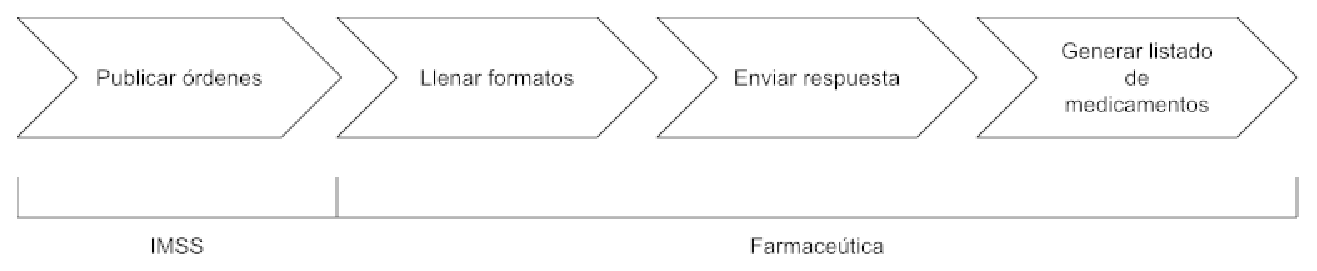
\includegraphics[scale=0.3]{flujo-proceso-contestar} 
\caption{Flujo del proceso para contestar órdenes de reposición.}
\label{fig:flow-proc-contestar}
\end{figure}

\item \textbf{Verificación de órdenes de reposición canceladas}: dado que el \textit{Instituto} tiene la facultad de cancelar las órdenes aún cuando ya hayan sido enviadas, es importante para el proveedor evitar el gasto extra que implica el envío de medicamento no solicitado por el \textit{Instituto} ya que implica un gasto extra el retirarlo. El operador accede al \textit{Sistema de Abastecimiento} de la misma manera dirigiéndose a la sección de \textit{Consulta de Órdenes} donde el operador provee información para realizar la búsqueda (rango de fechas de emisión\footnote{Fecha en que la orden fue realizada.}, el estado de la orden como ``cancelada'') y como resultado de esta búsqueda se muestra un listado con las órdenes que cumplen con tal filtro, así el operador copia la lista en un documento local en su equipo personal, para posteriormente realizar de forma manual tal filtro, con el fin de obtener las órdenes de reposición que han sido canceladas de las cuales no se tenía conocimiento. En la Figura \ref{fig:flow-proc-verificar} se muestra el proceso para verificar las órdenes de reposición canceladas.
\begin{figure}[H]
\centering
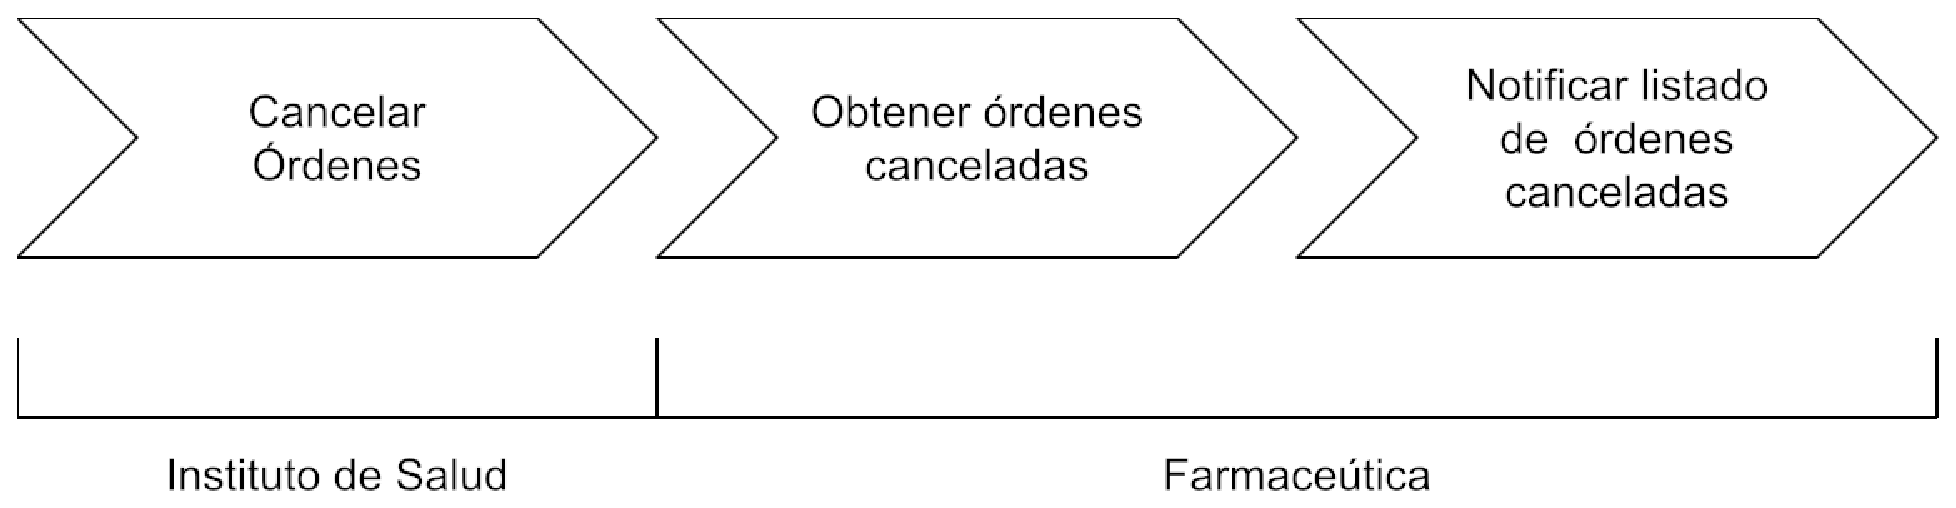
\includegraphics[scale=0.3]{flujo-proceso-verificar} 
\caption{Flujo del proceso para verificar órdenes de reposición canceladas.}
\label{fig:flow-proc-verificar}
\end{figure}
\end{enumerate}

El proveedor\footnote{Quien requiere automatizar la interacción con el Sistema de Abastecimiento para el envío de las órdenes de reposición y la verificación de órdenes canceladas.} representa a la compañía farmacéutica, por lo que en este documento nos referiremos al proveedor como a la compañía farmacéutica, o simplemente farmacéutica de manera indistinta. Los requerimientos funcionales del proveedor son la automatización de las tareas de interacción del operador con el \textit{Sistema de Abastecimiento} y la elaboración de reportes estadísticos sobre las órdenes de reposición procesadas durante la automatización.

\section{Objetivos}
\subsection{Objetivo principal}\label{sec:objetivo-principal}
Realizar un sistema de cómputo, de ahora en adelante llamado \textbf{AutoSA}, que reduzca el tiempo para contestar las órdenes de reposición, ayudando a mejorar, a su vez el tiempo que toma a la farmacéutica atender las órdenes de reposición, esto implica una reducción en tiempo desde que la orden es publicada en el \textit{Sistema de Abastecimiento} hasta que el medicamento es entregado físicamente al \textit{Instituto}.\\
El uso del sistema AutoSA evita el envío de medicamentos que ya no son solicitados, minimizando el consumo de recursos innecesarios, así como el tiempo que toma retirar del \textit{Instituto} tales medicamentos cancelados.\\
Dado que la farmacéutica atiende las órdenes de reposición del \textit{Instituto} en el doble de tiempo que su competencia, en particular contestar estas órdenes en el \textit{Sistema de Abastecimiento} requiere de tres personas dedicadas exclusivamente a ello, y un día completo el terminar esta parte del proceso. La solución propuesta para acelerar la respuesta y verificación de órdenes de reposición del \textit{Sistema de Abastecimiento} se encuentra programado por agentes\footnote{Agente dentro de este trabajo se refiere a las rutinas que automatizan los procesos realizados por los operadores del \textit{Sistema de Abastecimiento}.}, cada agente se dedica a emular las acciones del operador de la farmacéutica, el cual es el responsable de contestar o verificar las órdenes de reposición. El sistema AutoSA cuenta con una base de datos donde se almacenen los datos capturados por lo agentes durante la respuesta de órdenes, y una interfaz gráfica donde los trabajadores de la farmacéutica puedan realizar tareas de administración como son: la búsqueda, edición de órdenes de reposición y generación de reportes de las órdenes atendidas por los agentes.
\subsection{Objetivos secundarios}\label{sec:objetivos-secundarios}
\begin{enumerate}
\item Reducción del error humano en relación a la manipulación de la información.
\item Ahorro de recursos en la entrega de medicamentos no solicitados.
\item Reducción de tiempo en cuanto a la respuesta de órdenes de reposición.
\item Consistencia en los datos respecto a la generación de reportes estadísticos sobre las órdenes de reposición procesadas.
\end{enumerate}
Por lo anterior los afiliados del \textit{Instituto} se verán beneficiados, pues los medicamentos estarán disponibles con mayor frecuencia en las clínicas y hospitales.

\section{Descripción general de trabajo}\label{sec:desc-general}
La farmacéutica dedica diariamente un equipo constituido por tres personas durante toda la jornada laboral, dependiendo del volumen de órdenes de reposición emitidas por el \textit{Instituto} se puede agregar una persona más al equipo, para completar las tareas de envío de órdenes de reposición y verificar las órdenes de reposición canceladas dentro del \textit{Sistema de Abastecimiento}.\\
A través del proyecto de automatización se pretenden optimizar los siguientes puntos:
\begin{itemize}
\item Reducción del esfuerzo de recursos humanos.
\item Eliminar los errores de captura.
\item Reducción del tiempo dedicado al envío de las órdenes de reposición.
\item Detectar con rapidez las órdenes de reposición que hayan sido canceladas.
\end{itemize}
La necesidad de automatización de los procesos (Figuras \ref{fig:flow-proc-contestar} y \ref{fig:flow-proc-verificar}) antes mencionados pronostican una reducción de costos por devolución de medicamento no solicitado para el cliente y también la disminución de pérdidas en las ventas por solicitudes no atendidas en los rangos de tiempo acordados con el comprador. Dado lo anterior, se plantea un proyecto de software que cubra las necesidades de automatización y pueda ser administrado por usuarios no especializados en computación.\\
Para resolver el desarrollo del proyecto, el sistema AutoSA se divide en módulos con funcionalidades específicas que se muestran a continuación:
\begin{enumerate}
\item \textbf{Automatización de interacción con el Sistema de Abastecimiento}. La automatización de la interacción con el \textit{Sistema de Abastecimiento} consiste en replicar los pasos que sigue una persona de la farmacéutica (operador) encargada de llenar y extraer información de las órdenes de reposición del \textit{Sistema de Abastecimiento}, es decir, listar los pasos que sigue el operador cuando contesta las órdenes de reposición, describir las reglas de negocio necesarios para llenar los formularios que presenta el \textit{Sistema de Abastecimiento} al responder una orden de reposición. Por último se identifican las fuentes de los datos que se ocupan para llenar tales formularios y se define la forma de almacenamiento de la información necesaria de cada formulario.
\item \textbf{Generación de reportes}. La generación de reportes consiste en plasmar la información obtenida de las órdenes de reposición contestadas en el módulo anterior. La farmacéutica tiene ya una plantilla que se utiliza para pasar los pedidos a otras áreas, con el fin de continuar la atención de las órdenes de reposición; además de obtener estadísticas relacionadas con la cantidad de órdenes de reposición atendidas y canceladas.
\item \textbf{Interfaz de usuario}. La interfaz de usuario se refiere a la aplicación que muestra una interfaz gráfica en la cual los operadores de la farmacéutica pueden solicitar la generación de reportes; hacer consultas y modificaciones a las órdenes de reposición atendidas por el primer módulo.
\end{enumerate}

\subsection{Arquitectura de la solución}
Una definición de arquitectura de software es dada por Bourque\cite{SWEBOOK}:
\begin{quote}
El conjunto de estructuras necesarias para la comprensión de un sistema en el cual se comprometen elementos de software, relaciones entre ellos y sus propiedades.
\end{quote}
Esta definición expone que los requerimientos del cliente se traducen en especificaciones técnicas para los desarrolladores. Aplicando la definición anterior al presente proyecto donde tenemos los siguientes componentes (Figura \ref{fig:dia-arq-comp}):
\begin{figure}[h]
\centering
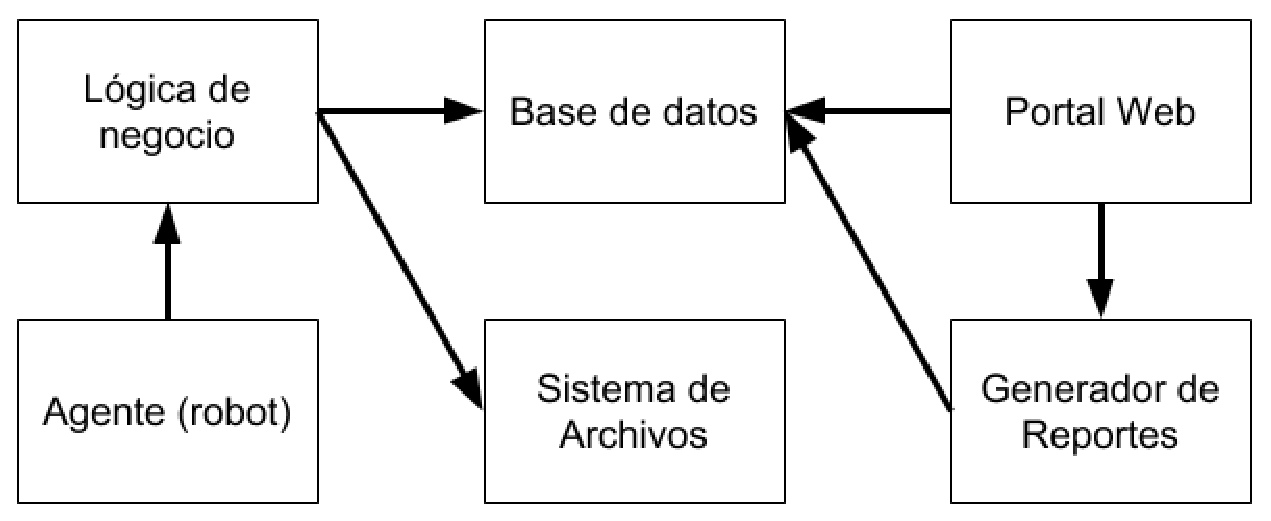
\includegraphics[scale=0.5]{dia-arq-comp} 
\caption{Módulos de la arquitectura.}
\label{fig:dia-arq-comp}
\end{figure}

\begin{itemize}
\item \textbf{Agente (robot)}. Interactúa directamente con el \textit{Sistema de Abastecimiento}, es el componente que automatiza las acciones de los operadores humanos de la farmacéutica.
\item \textbf{Lógica de Automatización}. Son bibliotecas y rutinas que se encargan de prestar los servicios necesarios al agente para su funcionamiento, permite comunicación con la base de datos, guarda las capturas de pantalla en el sistema de archivos y provee la configuración de inicio al agente.
\item \textbf{Persistencia}. Es el componente que se encarga de llevar la persistencia de los datos obtenidos durante la respuesta a las órdenes de reposición.
\item \textbf{Ficheros}. Este componente es el encargado de manejar operaciones con el sistema de archivos para almacenar las capturas de pantalla al momento de enviar la respuesta de cada orden de reposición.
\item \textbf{Generador de Reportes}. Este módulo está encargado de la generación de reportes tales como: órdenes de reposición atendidas, canceladas y formatos de órdenes de reposición enviadas.
\item \textbf{Portal Web}. Portal mediante el cual los usuarios pueden hacer correcciones a los datos obtenidos de las órdenes de reposición, reimprimir el formato de envío de la orden de reposición  y descargar los reportes generados por el módulo generador de reportes.
\end{itemize}

\subsection{Metodología utilizada}
El proyecto es abordado con la metodología \textit{Scrum}, la cual es un marco de trabajo para desarrollar, entregar y mantener productos complejos. Ésta consiste en un conjunto de roles, eventos, artefactos y reglas que los ligan. \textit{Scrum} da un enfoque adaptivo mientras promueve la entrega continua de soluciones y divide el desarrollo en ventanas de tiempo llamadas \textit{sprint}\cite{scrum}.\\
Dentro de \textit{Scrum} destacan los siguientes roles utilizados para el desarrollo del proyecto AutoSA\cite{scrum}:
\begin{itemize}
	\item \textit{Product Owner}: es responsable de maximizar el valor del producto que resulta del trabajo del \textit{Development Team}. Es la persona encargada de mantener el conjunto de tareas pendientes para futuros \textit{sprints}.
	\item \textit{Development Team}: es un grupo de profesionales encargado de realizar el trabajo necesario para completar las entregas de cada \textit{sprint}.
	\item \textit{Scrum Master}: es la persona responsable de promover y soportar \textit{Scrum} como está definido en la guía de \textit{Scrum}. Es un líder servil para el \textit{Scrum Team} que auxilia a este último a maximizar el valor del producto creado y ayuda a los involucrados en el desarrollo a comprender \textit{Scrum}.
	\item \textit{Scrum Team}: es conformado por el \textit{Product Owner}, el \textit{Development Team} y el \textit{Scrum Master}. \textit{Scrum Team} es un equipo de trabajo autoorganizado y multifuncional. Está diseñado para optimizar la flexibilidad, creatividad y productividad sin depender de personas ajenas al equipo.
	\item \textit{Stakeholder}: esta definición proviene directamente de su significado en inglés, es decir refiere a las personas que tienen interés en el producto.
\end{itemize}
El grupo de trabajo (\textit{Scrum Team}) formado por la consultora para el proyecto AutoSA consta de dos personas:
\begin{enumerate}
	\item Desarrollador\footnote{El autor del presente documento es la persona que cumplió con este rol durante todo el desarrollo del proyecto AutoSA.}: es la persona que cumple con las funciones siguientes:
	\begin{enumerate}
		\item Levantar los requerimientos de los \textit{stakeholders} de la farmacéutica.
		\item Cumplir con el rol de \textit{Product Owner} al ser encargado de mantener la lista de tareas para los \textit{sprints} futuros.
		\item Hacer investigación sobre tecnologías adecuadas para el desarrollo.
		\item Realizar el diseño e implementación de los componentes del sistema AutoSA.
		\item Formar parte del \textit{Scrum Team}.
	\end{enumerate}
	\item Arquitecto de software: tiene las siguientes responsabilidades:
	\begin{enumerate}
		\item Supervisar y aprobar el diseño e implementación realizado por el desarrollador.
		\item Hacer investigación sobre tecnologías adecuadas para el desarrollo.
		\item Cumplir con el rol de \textit{Scrum Master}.
		\item Formar parte del \textit{Scrum Team}.
	\end{enumerate}
\end{enumerate}
El proyecto fue planeado para ser realizado de julio a diciembre de 2014. Su conclusión es la liberación del sistema AutoSA que consiste en el despliegue total de los módulos en el ambiente productivo provisto por la farmacéutica, dando como resultado los siguientes productos:
\begin{itemize}
\item Rutinas para la generación de objetos en base de datos.
\item Rutinas para la creación de la estructura de directorios en el sistema de archivos.
\item Archivos de configuración propios de cada módulo.
\item Herramienta y rutinas de automatización.
\item Bibliotecas del portal web.
\item Manual de instalación y de usuario.
\item Capacitación a usuarios finales.
\end{itemize}
 
\section{Resumen}
El \textit{Instituto de Salud} mediante su \textit{Sistema de Abastecimiento} realiza las órdenes de reposición de medicamentos a las farmacéuticas, estas últimas invierten veinticuatro horas hombre por día para lograr contestar todas las órdenes de reposición, si se pudiera reducir el tiempo en que se atienden significaría un aumento en la velocidad de respuesta de la farmacéutica para entregar los medicamentos a centros de salud del \textit{Instituto}, motivo por el cual le interesa automatizar esta parte. El sistema AutoSA que se propone en este documento da solución mediante dos subsistemas: uno que automatiza los procedimientos de interacción con el \textit{Sistema de Abastecimiento} y otro que permite a los operadores de la farmacéutica generar reportes y acceder a datos de las órdenes de reposición atendidas.

\chapter{Análisis y alcance del proyecto}\label{cap2}


%===============================================================================
%===============================================================================


\section{Análisis de requerimientos}
En general, los requerimientos hablan de lo que se espera de una aplicación, tales requerimientos se clasifican en requerimientos funcionales y no funcionales:
\begin{itemize}
\item \textbf{Requerimientos funcionales}: descripciones detalladas de las funciones deseadas del proyecto. \cite{WileyBegSE}
\item \textbf{Requerimientos no funcionales}: descripciones de la calidad y capacidades del comportamiento del proyecto. \cite{WileyBegSE}
\end{itemize}
A modo de ejemplo se muestra el caso de la generación de reportes: un requerimiento funcional habla de los datos que debe capturar un usuario para obtener un reporte (fechas de inicio y término, número de orden, etcétera), mientras que un requerimiento no funcional habla sobre el formato de salida, verificación de permisos de usuario para generar el reporte,  capacidad del sistema para atender generación simultánea de varios reportes.


\subsection{Requerimientos funcionales}
\subsubsection{Automatizar el proceso para contestar órdenes de reposición}
Automatizar la interacción del operador de la farmacéutica que se realiza utilizando el portal SAI para contestar las órdenes de reposición, esto implica almacenar los datos de las órdenes de reposición que son utilizados para generar el formato de salida que es entregado al almacén para continuar con la atención de las órdenes (ver Figura \ref{fig:flow-proc-contestar}).

\subsubsection{Automatizar el proceso para cotejar órdenes de reposición canceladas}
Automatizar la interacción del operador de la farmacéutica que realizar para conocer las órdenes de reposición que han sido canceladas recientemente por el IMSS (ver Figura \ref{fig:flow-proc-verificar}).

\subsubsection{Interfaz WEB para la administración de órdenes de reposición contestadas}
Salvo lo referente a los procesos automatizados de los operadores de la farmacéutica, todos los requerimientos de administración de órdenes de reposición y generación de reportes deben ser accedidos mediante una interfaz web protegida por nombre de usuario y contraseña, como se muestra en la Figura \ref{fig:maq-login}.
\begin{figure}[h]
  \centering
  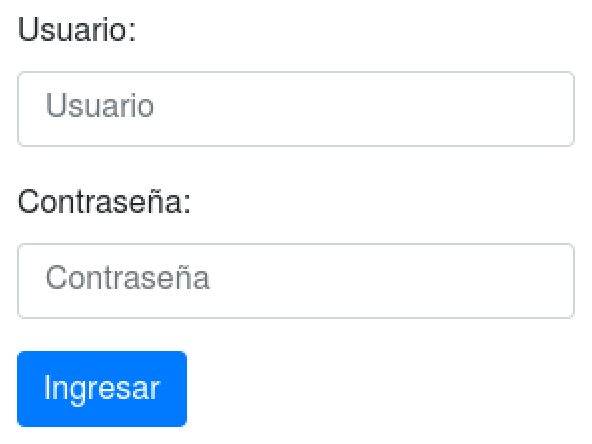
\includegraphics[scale=0.5]{maq-login} 
  \caption{Maqueta del acceso a la interfaz web.}
  \label{fig:maq-login}
\end{figure} 

\subsubsection{Búsqueda de órdenes de reposición}
En la interfaz web debe existir la posibilidad de buscar entre las órdenes de reposición contestadas mediante el número de orden de reposición, esta opción entrega solo una orden de reposición, o por un intervalo de fechas entre las cuales fueron atendidas las órdenes de reposición y entrega el listado de todas las órdenes de reposición que fueron respondidas en dicho intervalo. Las órdenes resultantes de la búsqueda deben ofrecer la opción para visualizar la información almacenada durante el proceso de contestación, como se muestra en la Figura \ref{fig:maq-search}
\begin{figure}[h]
  \centering
  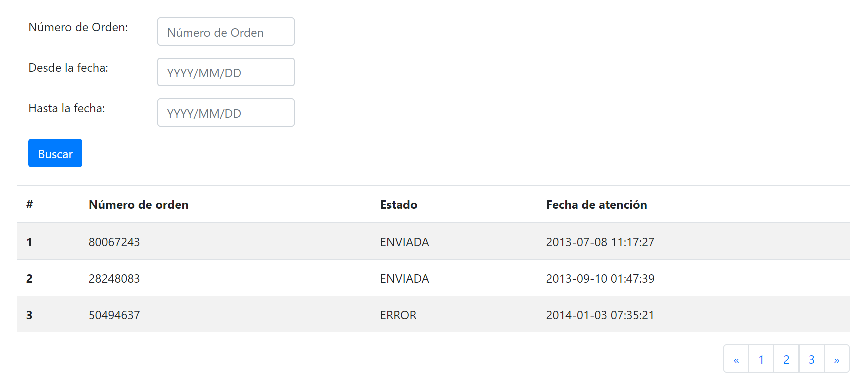
\includegraphics[width=\textwidth]{maq-search} 
  \caption{Maqueta de la búsqueda de ordenes.}
  \label{fig:maq-search}
\end{figure} 

\subsubsection{Visualización de orden de reposición}
La interfaz WEB debe tener una sección donde se muestre el contenido de una orden de reposición almacenada en la base de datos (ver Figura \ref{fig:maq-crud}), esta vista es individual, (no es posible mostrar el contenido de más de una orden de reposición). Además debe ofrecer las opciones para modificar los datos de la orden (ver requerimiento \ref{req-edicion}) y para generar el acuse de envío.
\begin{figure}[h]
  \centering
  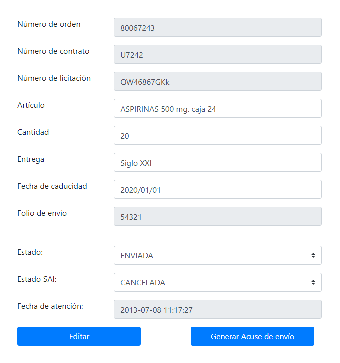
\includegraphics[scale=1]{maq-crud} 
  \caption{Maqueta del formulario para ver la información de una orden de reposición.}
  \label{fig:maq-crud}
\end{figure} 

\subsubsection{Edición de órdenes de reposición}\label{req-edicion}
Similar a la forma de mostrar la información de una orden de reposición, la interfaz web debe contar con una vista que permita la modificación de una orden de reposición (ver Figura \ref{fig:maq-crud}), esta vista debe ser única (no es posible modificar más de una orden de reposición), así mismo no será posible modificar datos como el número de orden y fecha de atención.

\subsubsection{Generación de reporte de órdenes de reposición contestadas}
El reporte con órdenes de reposición contestadas debe ser acotado entre fechas con precisión de horas (ver Figura \ref{fig:maq-report}), tal reporte, como su nombre lo indica, contiene los números de orden de reposición y datos definidos por la farmacéutica\footnote{Por acuerdo de confidencialidad no se enunciarán los datos contenidos en los reportes.}
\begin{figure}[h]
  \centering
  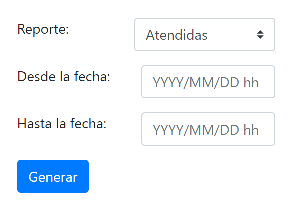
\includegraphics[scale=1.2]{maq-report} 
  \caption{Maqueta de la generación de reportes.}
  \label{fig:maq-report}
\end{figure} 

\subsubsection{Generación de formato de salida}
Este formato contiene datos con las órdenes de reposición y relaciones con claves de producto y centros de salud. El reporte está acotado por un intervalo de fechas con precisión de horas (ver Figura \ref{fig:maq-report}) \footnote{Por acuerdo de confidencialidad no se enunciarán los datos contenidos en el formato de salida así como el contenido de los catálogos de claves de producto y centros de salud.}.

\subsubsection{Generación de reporte con las órdenes de reposición canceladas reciéntemente}
Genera un reporte con las órdenes de reposición canceladas recientemente (ver Figura \ref{fig:maq-report}), es decir, las órdenes de reposición que tienen el estado de “cancelada” y no se han marcado como canceladas en el proceso de respuesta.

\subsubsection{Actualización de estatus de órdenes de reposición canceladas}
La actualización del estatus de las órdenes de reposición canceladas quiere decir que al sistema se le ``alimenta'' de forma masiva mediante un archivo con los números de las órdenes de reposición que han sido canceladas y se ha notificado al área correspondiente de la farmacéutica para cancelar la atención de dichas órdenes.

\subsubsection{Actualización de catálogos}
Alimentar de forma masiva, mediante un archivo separado por comas, los catálogos con claves de medicamentos, centros de salud y claves propias del manejo de la farmaceútica. Los catálogos definidos para la operación del sistema AutoSAI no podrán ser actualizados, por ejemplo, los catálogos que contienen los estados posibles de una orden de reposición cuando dentro del flujo de atención (ver Figura \ref{fig:dia-estados-orden}).


\subsection{Requerimientos no funcionales}
El cliente ha solicitado que el proyecto se apegue a su infraestructura, para conservar el acuerdo de confidencialidad y evitar exponer al cliente a riesgos de seguridad informática, no se enunciarán las versiones y tipo de infraestructura utilizada:
\begin{enumerate}
\item Sistema operativo capaz de ejecutar el software Java Virtual Machine (JVM).
\item Base de datos relacional SQL.
\item Uso de la herramienta Sahi para automatizar interacción con portal web SAI.
\item Las contraseñas de los usuarios para el acceso a la interfaz web deben ser almacenadas de forma segura, es decir, cifradas mediante una función hash.
\end{enumerate}


\subsection{Alcance del Proyecto}
%definir alcance
\begin{itemize}
\item El desarrollo de automatizar el proceso para contestar órdenes de reposición inicia con la ejecución del agente.
\item Queda fuera de alcance la verificación de existencia del medicamento en bodega.
\item Queda fuera de alcance la ejecución en paralelo de más de una instancia del proceso para contestar órdenes de reposición.
\item Queda fuera de alcance la ejecución en paralelo de más de una instancia del proceso para cotejar órdenes de reposición canceladas.
\item Queda fuera del desarrollo la administración de usuarios de la interfaz WEB mediante esta misma.
\item Queda fuera de alcance la ejecución simultánea de los procesos para contestar órdenes de reposición y cotejar órdenes de reposición canceladas.
\item Queda fuera de alcance la realización de respaldos de la información contenida en la base de datos o en el sistema de archivos.
\end{itemize}


\subsection{Riesgos asociados al proyecto}
%definir riesgos
\begin{itemize}
\item Al no contar con un ambiente de pruebas del portal SAI todos los datos alterados durante la programación de las rutinas de automatización podrían persistir información incorrecta, entonces es necesario mantener siempre un registro de las órdenes de reposición alteradas durante el desarrollo de las rutinas de automatización.
\item La herramientas de automatización se sustentan en la estructura DOM de las páginas HTML por las que navegan, entonces si ocurriera un cambio en dicha estructura las rutinas de automatización podrían dejar de funcionar.
\item El uso de software libre no tiene garantía por lo cual se reconoce como riesgo el fallo de software desarrollado por terceros.
\end{itemize}


%===============================================================================
%===============================================================================


\section{Casos de uso}
Un caso de uso es la representación de las posibles interacciones entre el sistema y sus actores, entendiendo un actor como una instancia (usuario u otro sistema). Así mismo, un caso de uso describe la funcionalidad del sistema por medio de mensajes y respuestas entre el actor y el sistema\cite{ApressSE}. A continuación se muestra el diagrama de casos de uso del sistema AutoSAI.

\begin{figure}[h]
  \centering
  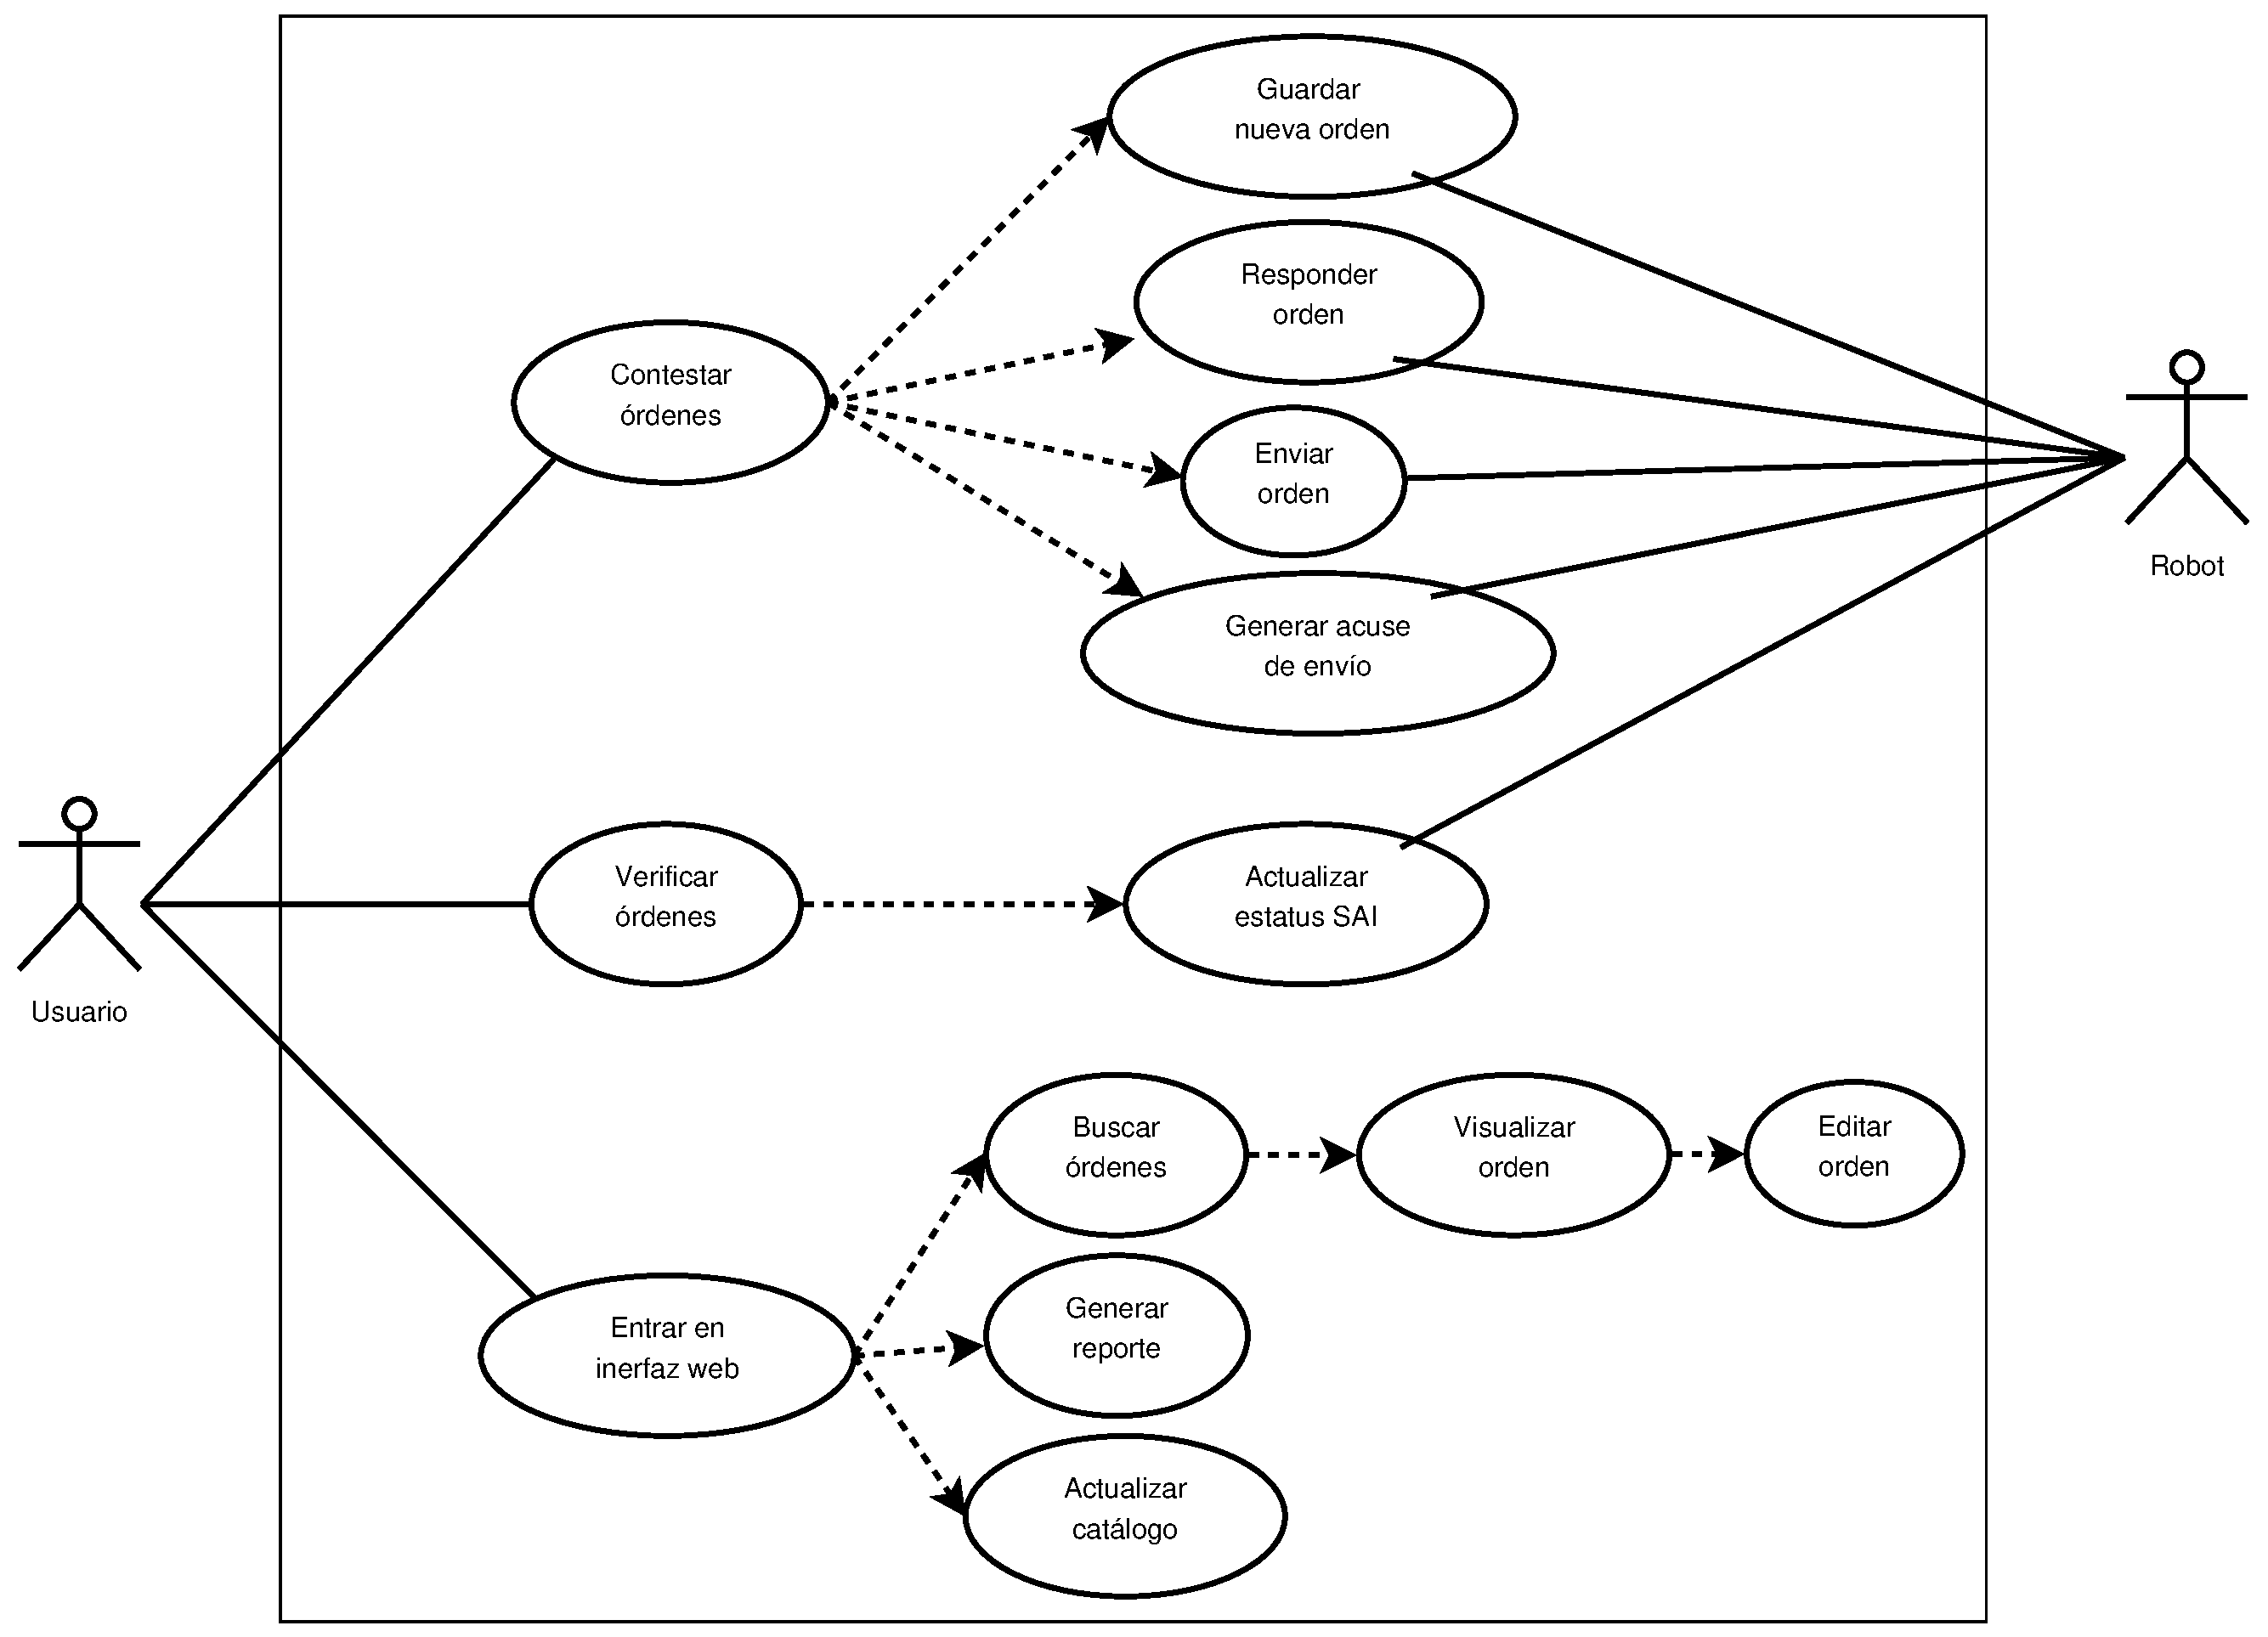
\includegraphics[width=\textwidth]{dia-casos-uso} 
  \caption{Diagrama de casos de uso.}
  \label{fig:dia-casos-uso}
\end{figure}

Con el fin de explicar mejor el flujo de atención de una orden de reposición es necesario mostrar el diagrama de estados de una orden de reposición durante el flujo de \textbf{envío de órdenes de reposición} (ver sección \ref{sec:intro-contexto}). Los estados que puede tomar una orden (ver Figura \ref{fig:dia-estados-orden}) indican:
\begin{itemize}
  \item Si la solicitud está lista para ser procesada: \textbf{Nueva}, \textbf{Contestada}.
  \item Si está siendo procesada: \textbf{Siendo Contestada}, \textbf{Siendo Enviada}.
  \item Si ha terminado el ciclo correctamente: \textbf{Enviada}.
  \item Si ha terminado el ciclo con errores: \textbf{Error}.
\end{itemize} 

\begin{figure}[h]
  \centering
  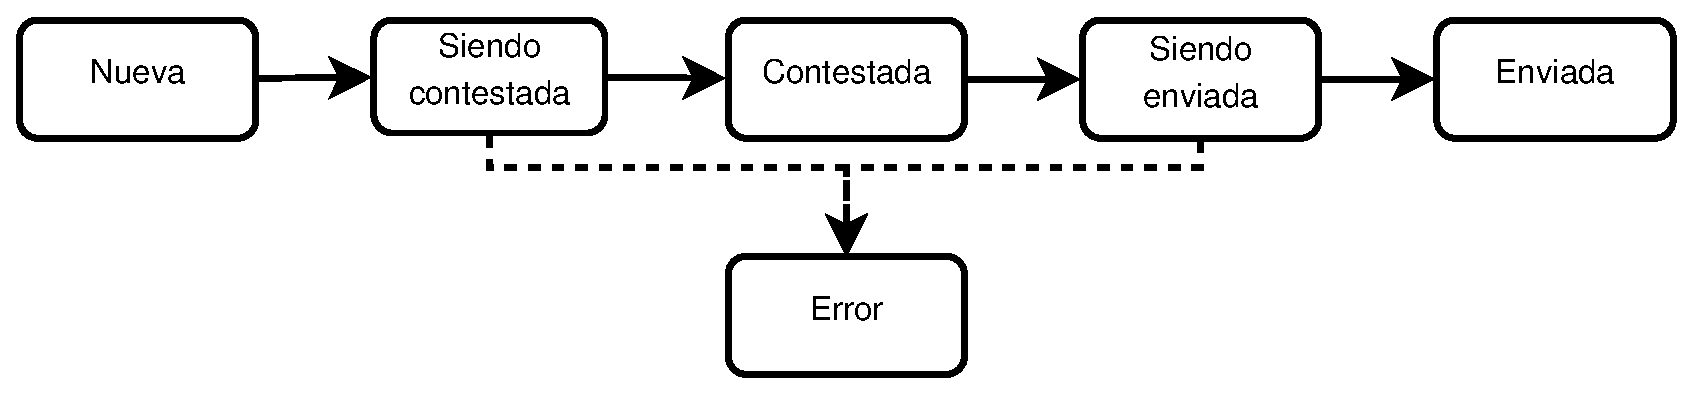
\includegraphics[width=\textwidth]{dia-estados-orden} 
  \caption{Diagrama de estados de una orden de reposición durante la ruta de respuesta de órdenes de reposición.}
  \label{fig:dia-estados-orden}
\end{figure}

Es importante mencionar que en las siguientes descripciones de caso de uso no se hará referencia al contenido exacto de las páginas así como el nombre de los campos, únicamente se hará mención de los campos necesarios para dar una explicación clara del caso.

\subsection{Contestar órdenes}
\paragraph{Identificador}
CU-CONTESTAR
\paragraph{Actores}
Usuario
\paragraph{Descripción}
El procedimiento completo para contestar las órdenes de reposición listadas en el portal SAI del IMSS (ver Figura \ref{fig:flow-proc-contestar}), el alcance de este caso comprende el acceso al portal SAI, contestar y enviar las órdenes de reproducción almacenando los datos y generando la captura de pantalla de dichas órdenes.\\
Queda fuera de alcance la obtención del reporte con las órdenes de reposición que han sido canceladas recientemente es cubierto por el caso de uso Generación de Reportes.
\paragraph{Precondiciones}
\begin{enumerate}
  \item El portal SAI se encuentra funcionando correctamente.
  \item El usuario cuenta con las credenciales para ingresar al portal SAI.
\end{enumerate}
\paragraph{Secuencia normal}
\begin{enumerate}
  \item Inicia sesión en portal SAI: provee nombre de usuario y le solicita al usuario ingresar la contraseña.
  \item Dirige el explorador a la pantalla donde se encuentra el listado con las órdenes de reposición que no han sido contestadas.
  \item Para cada orden de reposición del listado que se muestra se aplica el caso de uso CU-GUARDAR-NUEVA.
  \item Para cada solicitud en la base de datos con estado \textbf{Nueva} se aplican los casos de uso:
  \begin{enumerate}
    \item CU-RESPONDER-ORDEN.
  \end{enumerate}
  \item Para cada solicitud con estatus \textbf{Contestada}:
  \begin{enumerate}
    \item CU-ENVIAR-ORDEN
    \item CU-GENERAR-ACUSE
  \end{enumerate}
  \item El programa se repite desde el paso 2 hasta terminar las solicitudes sin contar las marcadas con estatus \textbf{Error}.
  \item Registra el fin del procedimiento en la base de datos.
\end{enumerate}
\paragraph{Postcondiciones}
\begin{enumerate}
  \item Todas las órdenes de reposición listadas han sido contestadas y enviadas.
  \item Se han registrado todas las ordenes de reposición atendidas en la base de datos.
  \item Los acuses de envió de las órdenes de reposición se encuentran en el sistema de archivos.
\end{enumerate}
\paragraph{Excepciones}
\begin{enumerate}
  \item Si en algún momento se detecta la pérdida de sesión en la página SAI, se reinicia el procedimiento desde el paso 1.
  \item Cualquier error durante la ejecución de este caso de uso será registrado en la bitácora el sistema.
\end{enumerate}


\subsection{Guardar nueva orden}
\paragraph{Identificador}
CU-GUARDAR-NUEVA
\paragraph{Actores}
Robot
\paragraph{Descripción}
Una orden de reposición es almacenada por primera vez con la información que se muestra en el listado de órdenes de reposición.
\paragraph{Precondiciones}
\begin{enumerate}
  \item Se tiene indicado un renglón del listado de órdenes de reposición sobre el cuál se realizará este caso de uso.
\end{enumerate}
\paragraph{Secuencia normal}
\begin{enumerate}
  \item Del listado de órdenes de reposición, cada solicitud es ingresada a la base de datos con estatus \textbf{Nueva} y datos provenientes del listado:
  \begin{enumerate}
    \item Contrato.
    \item Solicitud.
    \item Número de orden.
    \item Fecha de expedición.
    \item Almacén destino.
    \item \textit{URL} de contestación.
    \item \textit{URL} de envío: generada reemplazando el parámetro en la \textit{URL} de contestación ``responde'' por ``envia''.
  \end{enumerate}
\end{enumerate}
\paragraph{Postcondiciones}
\begin{enumerate}
  \item La orden de reposición se encuentra almacenada en la base de datos.
\end{enumerate}
\paragraph{Excepciones}
\begin{enumerate}
  \item Si el listado muestra la URL de envío y la orden no ha sido almacenada, entonces la orden es almacenada con estado \textbf{Contestada} y se registra la \textbf{cantidad solicitada} en 0.
  \item Si ocurre algún error la orden es almacenada con estado \textbf{Error}.
\end{enumerate}


\subsection{Responder orden}
\paragraph{Identificador}
CU-RESPONDER-ORDEN
\paragraph{Actores}
Robot
\paragraph{Descripción}
En la pantalla para contestar una orden de reposición se llenan los formularios y se almacena la información de la pantalla en el registro de la base de datos que corresponde a la orden de reposición.
\paragraph{Precondiciones}
\begin{enumerate}
  \item Se indica una orden de reposición almacenada en la base de datos sobre la cual se aplica este caso de uso.
  \item La orden de reposición se encuentra almacenada en la base de datos.
  \item La orden de reposición tiene estado \textbf{Nueva}.
\end{enumerate}
\paragraph{Secuencia normal}
\begin{enumerate}
  \item Cambia el estado de la orden a \textbf{Siendo Contestada}.
  \item Dirige el explorador a la \textit{URL} de contestación (ver caso de uso CU-GUARDAR-NUEVA).
  \item Llena el formulario que se presenta en esta pantalla con las siguientes consideraciones:
  \begin{enumerate}
    \item Fecha de fabricación: primer día del año en curso si la fecha actual no es del mes de diciembre, en caso contrario se toma el año siguiente.
    \item Fecha de caducidad: último día del año en curso si la fecha actual no es del mes de diciembre, en caso contrario se toma el año siguiente.
  \end{enumerate}
  \item Activar el botón ``contestar'' del formulario de la orden de reposición.
  \item Cambia el estado de la orden a \textbf{Contestada}.
\end{enumerate}
\paragraph{Postcondiciones}
\begin{enumerate}
  \item Los formularios de la pantalla han sido completados correctamente.
  \item Los datos del formulario se encuentran almacenado en la base de datos.
  \item El estado de la orden en la base de datos es \textbf{Contestada}.
\end{enumerate}
\paragraph{Excepciones}
\begin{enumerate}
  \item Si ocurre algún error la orden es almacenada con estado \textbf{Error}.
\end{enumerate}


\subsection{Enviar orden}
\paragraph{Identificador}
CU-ENVIAR-ORDEN
\paragraph{Actores}
Robot
\paragraph{Descripción}
Enviar la orden de reposición contestada de regreso al portal SAI.
\paragraph{Precondiciones}
\begin{enumerate}
  \item Una orden de reposición registrada en la base de datos.
  \item La orden de reposición tiene estado \textbf{Contestada}.
\end{enumerate}
\paragraph{Secuencia normal}
\begin{enumerate}
  \item Cambia estado de la orden a \textbf{Siendo Enviada}.
  \item El explorador dirige a la \textit{URL de envío}.
  \item Guardar el folio de envío en la base de datos.
  \item Cambia estado de la orden a \textbf{Enviada}.
\end{enumerate}
\paragraph{Postcondiciones}
\begin{enumerate}
  \item El folio de envió de la orden de reposición se encuentra guardado en la base datos.
  \item El estado de la orden en la base de datos es \textbf{Enviada}.
\end{enumerate}
\paragraph{Excepciones}
\begin{enumerate}
  \item Si ocurre algún error la orden es almacenada con estado \textbf{Error}.
\end{enumerate}


\subsection{Generar acuse de envío}
\paragraph{Identificador}
CU-GENERAR-ACUSE
\paragraph{Actores}
Robot
\paragraph{Descripción}
Generar el acuse de envío de la orden de reposición.
\paragraph{Precondiciones}
\begin{enumerate}
  \item Una orden de reposición registrada en la base de datos.
  \item La orden de reposición tiene estado \textbf{Enviada}.
\end{enumerate}
\paragraph{Secuencia normal}
\begin{enumerate}
  \item Extraer la información de la orden de reposición de la base de datos.
  \item Mandar la generación del acuse de envío.
  \item Colocar el documento generado en el sistema de archivos.
\end{enumerate}
\paragraph{Postcondiciones}
\begin{enumerate}
  \item Un documento en el sistema de archivos que contiene el acuse de envío.
\end{enumerate}
\paragraph{Excepciones}
\begin{enumerate}
  \item En caso de algún error se registra el error en la bitácora del sistema (el usuario posteriormente podrá volver a imprimir el acuse, ver caso de uso CU-VISUALIZAR).
\end{enumerate}


\subsection{Verificar órdenes}
\paragraph{Identificador}
CU-VERIFICAR
\paragraph{Actores}
Usuario
\paragraph{Descripción}
Modelar el procedimiento automatizado para verificar órdenes de reposición canceladas (ver Figura \ref{fig:flow-proc-verificar}), el alcance de este caso de uso comprende el acceso al portal SAI, búsqueda de órdenes de reposición con estado \textbf{Cancelado} y comparación con la base de datos.\\
Queda fuera de alcance: la actualización masiva del estado de órdenes de reposición es cubierto en el caso de uso \textbf{CU-ACTUALIZAR-CATALOGO}; y la obtención del reporte con las órdenes de reposición que han sido canceladas recientemente es cubierto por el caso de uso \textbf{CU-GENERAR-REPORTE}.
\paragraph{Precondiciones}
\begin{enumerate}
  \item El portal SAI se encuentra funcionando correctamente.
  \item El usuario cuenta con las credenciales para ingresar al portal SAI.
\end{enumerate}
\paragraph{Secuencia normal}
\begin{enumerate}
  \item Inicia sesión en portal SAI: provee nombre de usuario y le solicita al usuario ingresar la contraseña.
  \item Dirige el explorador a la pantalla de búsqueda de órdenes de reposición.
  \item Llena el formulario para el filtro de búsqueda:
  \begin{enumerate}
    \item Rango de fechas que comprende los últimos siete días desde la fecha actual.
    \item Estado \textbf{Cancelada}.
  \end{enumerate}
  \item Del listado de órdenes de reposición resultantes genera una lista con el número de orden de cada renglón.
  \item Con el listado del paso anterior se realiza el caso de uso \textbf{CU-ACTUALIZAR-ESTATUS-SAI}.
\end{enumerate}
\paragraph{Postcondiciones}
\begin{enumerate}
  \item Se cuenta con la relación de órdenes de reposición atendidas por el sistema que han sido canceladas en el portal SAI y no se tenía conocimiento previo.
  \item Las órdenes de reposición publicadas en el portal SAI dentro de los últimos siete día a la fecha actual reflejan en la base de datos dentro del campo \textbf{Estado SAI} el estado de vigencia en el portal SAI.
\end{enumerate}
\paragraph{Excepciones}
\begin{enumerate}
  \item Cualquier error durante la ejecución de este caso de uso será registrado en la bitácora el sistema.
\end{enumerate}


\subsection{Actualizar estatus SAI}
\paragraph{Identificador}
CU-ACTUALIZAR-ESTATUS-SAI
\paragraph{Actores}
Robot
\paragraph{Descripción}
Actualizar en forma masiva el estado de atención en el portal SAI dentro de la base de datos del sistema AutoSAI.
\paragraph{Precondiciones}
\begin{enumerate}
  \item Se cuenta con una lista de órdenes de reposición.
  \item Las órdenes listadas tienen estado \textbf{Cancelada} en el portal SAI. 
\end{enumerate}
\paragraph{Secuencia normal}
\begin{enumerate}
  \item Actualiza el estado SAI de las órdenes de reposición en la base de datos.
\end{enumerate}
\paragraph{Postcondiciones}
\begin{enumerate}
  \item Las órdenes de reposición recibidas tienen estado \textbf{Cancelada} en el campo \textbf{Estado SAI} dentro de la base de datos.
\end{enumerate}
\paragraph{Excepciones}
\begin{enumerate}
  \item Las órdenes de reposición que no estén registradas en la base de datos se registrarán con campos nulos a excepción del número de orden.
  \item Cualquier error durante la ejecución de este caso de uso será registrado en la bitácora el sistema.
\end{enumerate}


\subsection{Entrar en interfaz Web}
\paragraph{Identificador}
CU-ENTRAR-WEB
\paragraph{Actores}
Usuario
\paragraph{Descripción}
Explicar la función que autoriza la entrada a la interfaz Web del sistema (ver Figura \ref{fig:dia-casos-uso}) donde los usuarios pueden hacer acciones de administración de las órdenes de reposición atendidas por las rutinas de automatización, generación de reportes y actualización de catálogos.
\paragraph{Precondiciones}
\begin{enumerate}
  \item El usuario se encuentra previamente registrado en el sistema.
  \item El usuario cuanta con credenciales vigentes para ingresar a la interfaz web.
\end{enumerate}
\paragraph{Secuencia normal}
\begin{enumerate}
  \item El sistema muestra la pantalla de acceso.
  \item El usuario ingresa los campos:
  \begin{enumerate}
    \item Nombre de usuario.
    \item Contraseña.
  \end{enumerate}
  \item El sistema busca el nombre de usuario en la base de datos
  \item El sistema compara la contraseña provista por el usuario con el valor almacenado en la base de datos.
  \item Muestra la pantalla de generación de reportes.
\end{enumerate}
\paragraph{Postcondiciones}
\begin{enumerate}
  \item El usuario cuenta con un código temporal de acceso a la interfaz web.
  \item Se muestra la pantalla de generación de reportes.
\end{enumerate}
\paragraph{Excepciones}
\begin{enumerate}
  \item En los siguientes esceneracios se concideran un error de autencación.
  \begin{itemize}
    \item El usuario no existe en la base de datos.
    \item El usuario tiene estado \textbf{deshabilitado}.
    \item La contraseña proporcionada no coincide con la almacenada. 
  \end{itemize}
\end{enumerate}

\subsection{Generar reporte}
\paragraph{Identificador}
CU-GENERAR-REPORTE
\paragraph{Actores}
Usuario
\paragraph{Descripción}
Este caso de uso ofrece al usuario la generación de reportes, es decir, ejecutar una consulta a la base de datos y vaciar el resultado en un archivo. La consulta puede ser ejecutada sobre una o más tablas, es importante mencionar que existen catálogos con claves de productos y clientes que cambian constantemente, ver caso de uso \textbf{CU-ACTUALIZAR-CATALOGO}.
\paragraph{Precondiciones}
\begin{enumerate}
  \item El usuario ha iniciado sesión correctamente en la interfaz web (ver caso de uso \textbf{CU-ENTRAR-WEB}).
\end{enumerate}
\paragraph{Secuencia normal}
\begin{enumerate}
  \item El usuario navega a la pantalla de generación de reportes.
  \item En la pantalla de generación de reportes el usuario realiza las siguientes acciones:
    \begin{enumerate}
    \item Llenar el formulario de la pantalla con los siguientes campos:
    \begin{enumerate}
      \item \textbf{Tipo de reporte}
      \item \textbf{Fecha y hora inicial}
      \item \textbf{Fecha y hora final}
    \end{enumerate}
    \item Enviar el formulario.
  \end{enumerate}
  \item El sistema ejecuta los siguientes pasos:
  \begin{enumerate}
    \item Realiza para consulta a la base de datos definida para el reporte requerido en 1.a.
    \item El resultado del paso anterior es escrito en un archivo extendido de Excel y depositado en el sistema de archivos.
    \item Muestra al usuario la ruta en el sistema de archivos donde fue depositado el reporte.
  \end{enumerate}
\end{enumerate}
\paragraph{Postcondiciones}
\begin{enumerate}
  \item El reporte se encuentra en el sistema de archivos dentro un archivo con formato extendido de Excel.
\end{enumerate}
\paragraph{Excepciones}
\begin{enumerate}
  \item Si el reporte no cuenta con registros el archivo no se genera y se muestra un mensaje al usuario indicando la situación.
\end{enumerate}


\subsection{Actualizar catálogo}
\paragraph{Identificador}
CU-ACTUALIZAR-CATALOGO
\paragraph{Actores}
Usuario
\paragraph{Descripción}
Define la actualización masiva de los catálogos en la base de datos mediante un archivo ingresado por un usuario de la interfaz Web.
\paragraph{Precondiciones}
\begin{enumerate}
  \item El usuario ha iniciado sesión correctamente en la interfaz web (ver caso de uso \textbf{CU-ENTRAR-WEB}).
  \item El archivo ingresado tiene formato extendido de Excel.
  \item Los catálogos que pueden ser modificados por este caso de uso son aquellos que contienen códigos de medicamentos y lugares de entrega.
\end{enumerate}
\paragraph{Secuencia normal}
\begin{enumerate}
  \item El usuario navega a la pantalla de administración de catálogos.
  \item El usuario realiza las siguientes acciones en la pantalla de administración de catálogos:
  \begin{enumerate}
    \item Seleccionar el nombre del catálogo.
    \item Seleccionar el archivo en formato de Excel que contiene la información para el catálogo.
    \item Enviar el formulario.
  \end{enumerate}
  \item El sistema sigue los siguientes pasos:
  \begin{enumerate}
    \item Valida el formato del archivo recibido.
    \item Valida que el archivo recibido contenga al menos un renglón sin contar el encabezado.
    \item Borra el contenido del catálogo en la base datos y copia la información del archivo recibido.
    \item Muestra al usuario el número de registros guardados en el catálogo después de la actualización.
  \end{enumerate}
\end{enumerate}
\paragraph{Postcondiciones}
\begin{enumerate}
  \item El catálogo ha sido actualizado al contenido del archivo proporcionado por el usuario.
\end{enumerate}
\paragraph{Excepciones}
\begin{enumerate}
  \item Si el archivo no cuanta con el formato solicitado, entonces se muestra un mensaje de error al usuario y se cancela la ejecución sin modificar el catálogo en la base de datos.
  \item Si el archivo no contiene ningún registro para el catálogo, entonces se muestra un mensaje de error al usuario y se cancela la ejecución sin modificar el catálogo en la base de datos.
\end{enumerate}


\subsection{Buscar órdenes}
\paragraph{Identificador}
CU-BUSCAR
\paragraph{Actores}
Usuario
\paragraph{Descripción}
\paragraph{Precondiciones}
\begin{enumerate}
  \item El usuario ha iniciado sesión correctamente en la interfaz web (ver caso de uso \textbf{CU-ENTRAR-WEB}).
\end{enumerate}
\paragraph{Secuencia normal}
\begin{enumerate}
  \item El usuario navega a la pantalla de búsqueda de órdenes de reposición.
  \item El usuario realiza ingresa los criterios para la búsqueda presentados en el filtro:
  \begin{enumerate}
    \item Número de orden.
    \item Estatus de atención.
    \item Rango de fechas en que fueron atendidas las órdenes de reposición.
  \end{enumerate}
  \item El sistema muestra el resultado de la búsqueda, para cada orden de reposición listada se muestra un enlace que lleva a la visualización de la orden (ver casos de uso \textbf{CU-VISUALIZAR}).
\end{enumerate}
\paragraph{Postcondiciones}
\begin{enumerate}
  \item Se muestra un listado con las órdenes de reposición que cumplen con el filtro definido por el usuario durante el caso de uso.
\end{enumerate}
\paragraph{Excepciones}
\begin{enumerate}
  \item En caso de no contar con conexión a la base de datos se muestra un mensaje de error informando al usuario.
\end{enumerate}


\subsection{Visualizar orden}
\paragraph{Identificador}
CU-VISUALIZAR
\paragraph{Actores}
Usuario
\paragraph{Descripción}
La forma en que el usuario de la interfaz web es capaz de visualizar los datos de una orden de reposición, para llegar a esta página es necesario que el usuario haya ejecutado la búsqueda de órdenes de reposición y seleccionado la orden para visualizar, como se muestra en la Figura \ref{fig:dia-casos-uso} (ver caso de uso \textbf{CU-BUSCAR}).
\paragraph{Precondiciones}
\begin{enumerate}
  \item El usuario ha iniciado sesión correctamente en la interfaz web (ver caso de uso \textbf{CU-ENTRAR-WEB}).
  \item El usuario localiza la orden de reposición que desea visualizar (ver caso de uso \textbf{CU-BUSCAR})
\end{enumerate}
\paragraph{Secuencia normal}
\begin{enumerate}
  \item El usuario navega a la pantalla de visualización de la orden de reposición seleccionada (ver caso de uso \textbf{CU-BUSCAR}).
  \item Se muestra la pantalla con los datos de la orden:
  \begin{enumerate}
    \item Se muestran todos los datos capturados del portal SAI durante el procedimiento de atención.
    \item También se muestran los estados de atención, es decir el estado en el portal SAI  y el estado de atención.
  \end{enumerate}
  \item Se muestran enlaces para que el usuario pueda editar los datos de la orden (ver caso de uso \textbf{CU-EDITAR}) y también para generar el acuse de envío (ver caso de uso \textbf{CU-GENERAR-ACUSE}).
  \item En caso de seleccionar la generación del acuse de envío se ejecuta el caso de uso \textbf{CU-GENERAR-ACUSE}.
\end{enumerate}
\paragraph{Postcondiciones}
\begin{enumerate}
  \item Se muestra una pantalla al usuario con los datos de la orden de reposición solicitada, además las opciones para editar y generar el acuse de envío.
\end{enumerate}
\paragraph{Excepciones}
\begin{enumerate}
  \item En caso de no contar con conexión a la base de datos se muestra un mensaje de error informando al usuario.
\end{enumerate}


\subsection{Editar orden}
\paragraph{Identificador}
CU-EDITAR
\paragraph{Actores}
Usuario
\paragraph{Descripción}
\paragraph{Precondiciones}
\begin{enumerate}
  \item El usuario ha iniciado sesión correctamente en la interfaz web (ver caso de uso \textbf{CU-ENTRAR-WEB}).
  \item El usuario visualiza la orden de reposición que desea editar (ver caso de uso \textbf{CU-VISUALIZAR}).
  \item Los campos utilizados para identificar unívocamente la orden de reposición no podrán ser modificados. 
\end{enumerate}
\paragraph{Secuencia normal}
\begin{enumerate}
  \item El usuario navega a la pantalla de edición con la orden de reposición visualizada (ver caso de uso \textbf{CU-VISUALIZAR}).
  \item Modificar cualquiera de los campos editables.
  \item Seleccionar el botón Guardar.
\end{enumerate}
\paragraph{Postcondiciones}
\begin{enumerate}
  \item Los datos modificados por el usuario en la interfaz web se encuentran almacenados en la base de datos.
\end{enumerate}
\paragraph{Excepciones}
\begin{enumerate}
  \item En caso de no contar con conexión a la base de datos se muestra un mensaje de error informando al usuario.
\end{enumerate}



\chapter{Diseño del proyecto}\label{cap3}
Conforme a lo visto en el capítulo anterior, el proyecto requiere ser ejecutado de dos formas distintas (ejecución de automatizaciones y portal de usuario), además necesita de una base de datos para mantener persistentes los datos de las órdenes de reposición atendidas, catálogos y datos de usuario, también es necesario acceso al sistema de archivo para guardar las capturas de pantalla de las órdenes de reposición enviadas. Por lo que es necesario dos ambientes de ejecución, la automatización que será ejecutada exclusivamente en el sistema operativo y la del web, que si bien también estará contenida en el sistema operativo es necesario que se ejecute parte del sistema en el explorador del usuario.


%===============================================================================
%===============================================================================


\section{Diseño de la arquitectura}
Bourque define la arquitectura de software como:\footnote{\textcolor{red}{Karla, como es cita textual (según mi propia traducción :P ) prefiero dejarla en un párrafo por separado mientras que lo que sea paráfrasis dejarlo en texto seguido ¿cómo ves?}}
\begin{quote}
	El conjunto de estructuras necesarias para la comprensión de un sistema en el cual se comprometen elementos de software, relaciones entre ellos y sus propiedades\cite{SWEBOOK}.
\end{quote}
En las últimas décadas la arquitectura de software ha profundizado en el estudio genérico de las estructuras del software, dando lugar a técnicas como los Patrones de Diseño (ver Apéndice \ref{sec-patrones}) \cite{SWEBOOK, SoftwareArchitectureInAction}.

\textcolor{red}{Karla, Quité las secciones de patrones de diseño, arquitectura 4+1, arquitectura orientada a servicios.}\footnote{\textcolor{red}{Karla, no sentí que los conceptos de patrones de diseño y arquitecturas encajara aquí, así que los mandé al apéndice de patrones de diseño y si los necesito durante este capítulo o el siguiente (implementación) nada más haré referencia ¿Qué opinas?}}

Siguiendo el concepto de arquitectura, dado anteriormente, a continuación se muestran los componentes del sistema y como dan solución a los casos de uso del Capítulo \ref{sec:casos-uso}.

\subsection{Componentes del sistema AutoSA}
El diagrama de componentes sirve para visualizar los componentes en los que se divide el sistema y las interfaces por las cuales se comunican tales componentes, el la Figura \ref{fig:dia-components} se muestra el diagrama de componentes para el sistema AutoSA. En las secciones consecuentes se describe cada componente y las interfaces que ofrece\footnote{Únicamente se mostrarán los diagramas de secuencia más completos que reflejan un comportamiento no trivial.}.
\begin{figure}[h]
\centering
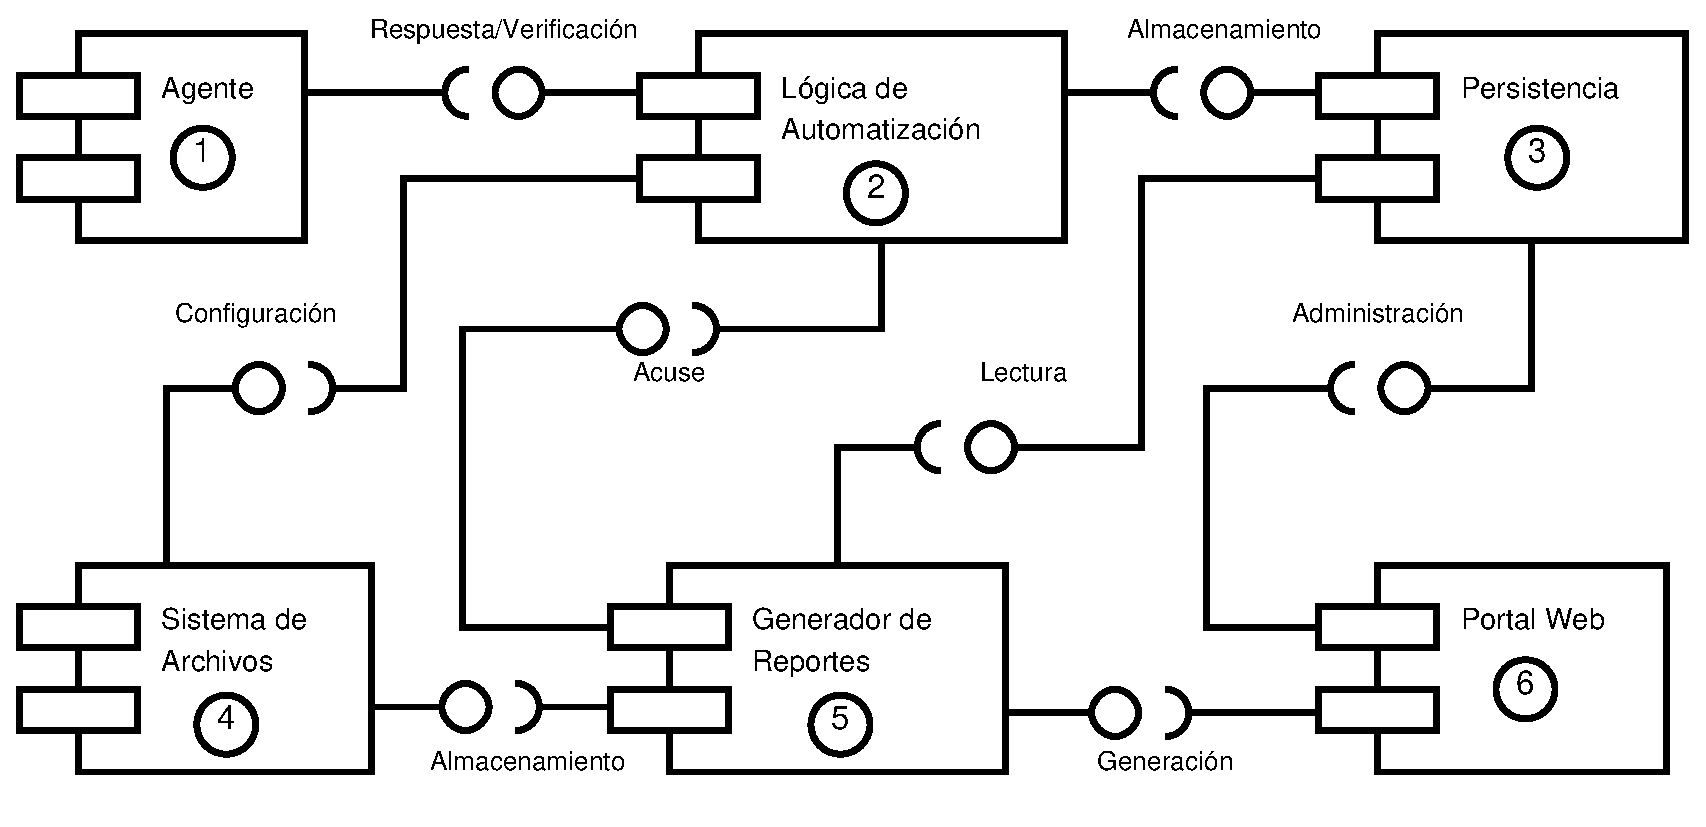
\includegraphics[width=\textwidth]{dia-components}
\caption{Diagrama de componentes.}
\label{fig:dia-components}
\end{figure}

\subsubsection{Agente}
El componente que contiene y ejecuta las rutinas de automatización, esto es mediante una interfaz con el usuario en la cual puede seleccionar el proceso a ser ejecutado. No ofrece interfaces a los demás componentes, consume exclusivamente el componente de Lógica de Automatización.

\subsubsection{Lógica de Automatización}
La función de este componente es de ejecutar las reglas de negocio necesarias para en los flujos de los procesos de automatización.  
\paragraph{Respuesta\\}
Provee el acceso a las reglas de negocio del proceso de respuesta de órdenes de reposición (ver caso de uso \ref{cu-contestar}).\\
\noindent
	\begin{tabular}{|p{\dimexpr.2\textwidth}|p{\dimexpr.8\textwidth-4\tabcolsep}|}
		\hline
		\textbf{Identificador}	& \textbf{guardar-orden-nueva}\\
		\hline
		\hline
		\textbf{Descripción}	& Guarda un listado de nuevas órdenes de reposición.\\
		\hline
		\textbf{Parámetros}		& \textbullet\, Listado de mapas, cada mapa contiene los datos de una orden de reposición.\\
		\hline
		\textbf{Resultado}		& No ofrece resultado.\\
		\hline
	\end{tabular}
	\vspace{3mm}\\
	\begin{tabular}{|p{\dimexpr.2\textwidth}|p{\dimexpr.8\textwidth-4\tabcolsep}|}
		\hline
		\textbf{Identificador}	& \textbf{obtener-orden-contestar}\\
		\hline
		\hline
		\textbf{Descripción}	& Da la siguiente orden de reposición para contestar.\\
		\hline
		\textbf{Parámetros}		& \textbullet\, No recibe parámetros.\\
		\hline
		\textbf{Resultado}		& Mapa con la información de la orden de reposición.\\
		\hline
	\end{tabular}
	\begin{longtable}{|p{\dimexpr.2\textwidth}|p{\dimexpr.8\textwidth-4\tabcolsep}|}
		\hline
		\textbf{Identificador}	& \textbf{obtener-datos-respuesta}\\
		\hline
		\hline
		\textbf{Descripción}	& Da los datos necesarios para llenar los formularios para contestar una orden de reposición en el Sistema de Abastecimiento.\\
		\hline
		\textbf{Parámetros}		& \textbullet\, Mapa con los datos de la orden para contestar.\\
		\hline
		\textbf{Resultado}		& Mapa con la información para llenar los formularios para contestar la orden de reposición.\\
		\hline
	\end{longtable}
	\begin{longtable}{|p{\dimexpr.2\textwidth}|p{\dimexpr.8\textwidth-4\tabcolsep}|}
		\hline
		\textbf{Identificador}	& \textbf{actualizar-orden-contestada}\\
		\hline
		\hline
		\textbf{Descripción}	& Actualiza los datos guardados de la orden de reposición con los datos de la respuesta en el  Sistema de Abastecimiento. Utiliza el componente de persistencia para actualizar los datos.\\
		\hline
		\multirow{2}{*}{\textbf{Parámetros}}	& \textbullet\, Número de orden.\\
												& \textbullet\, Mapa con los datos para guardar.\\
		\hline
		\textbf{Resultado}		& No ofrece resultado.\\
		\hline
	\end{longtable}
	\begin{longtable}{|p{\dimexpr.2\textwidth}|p{\dimexpr.8\textwidth-4\tabcolsep}|}
		\hline
		\textbf{Identificador}	& \textbf{obtener-orden-enviar}\\
		\hline
		\hline
		\textbf{Descripción}	& Da la siguiente orden de reposición para enviar.\\
		\hline
		\textbf{Parámetros}		& \textbullet\, No recibe parámetros.\\
		\hline
		\textbf{Resultado}		& Mapa con la información de la orden de reposición.\\
		\hline
	\end{longtable}
	\begin{longtable}{|p{\dimexpr.2\textwidth}|p{\dimexpr.8\textwidth-4\tabcolsep}|}
		\hline
		\textbf{Identificador}	& \textbf{guardar-orden-enviada}\\
		\hline
		\hline
		\textbf{Descripción}	& Actualiza los datos guardados de la orden de reposición con los datos de la pantalla de envío del Sistema de Abastecimiento. Utiliza el componente de persistencia para actualizar los datos.\\
		\hline
		\multirow{2}{*}{\textbf{Parámetros}}	& \textbullet\, Número de orden.\\
												& \textbullet\, Mapa con los datos para guardar.\\
		\hline
		\textbf{Resultado}		& No ofrece resultado.\\
		\hline
	\end{longtable}
	\begin{longtable}{|p{\dimexpr.2\textwidth}|p{\dimexpr.8\textwidth-4\tabcolsep}|}
		\hline
		\textbf{Identificador}	& \textbf{obtener-acuse-envio}\\
		\hline
		\hline
		\textbf{Descripción}	& Solicita la generación de el acuse de envío al componente de reportes y almacena el documento el componente de Sistema de Archivos.\\
		\hline
		\textbf{Parámetros}		& \textbullet\, Número de orden.\\
		\hline
		\textbf{Resultado}		& No ofrece resultado.\\
		\hline
	\end{longtable}
	\vspace{5mm}
\paragraph{Verificación\\}
Provee el acceso a las reglas de negocio del proceso de verificación de órdenes de reposición canceladas.

	\begin{longtable}{|p{\dimexpr.2\textwidth}|p{\dimexpr.8\textwidth-4\tabcolsep}|}
		\hline
		\textbf{Identificador}	& \textbf{obtener-rango-verificar}\\
		\hline
		\hline
		\textbf{Descripción}	& Obtiene el rango de fechas para ingresar en el formulario de búsqueda del Sistema de Abastecimiento. El número de días que comprende el rango se obtiene utilizando el componente de Sistema de archivos.\\
		\hline
		\textbf{Parámetros}		& \textbullet\, No tiene parámetros.\\
		\hline
		\textbf{Resultado}		& El número de días para el rango de búsqueda.\\
		\hline
	\end{longtable}

	\begin{longtable}{|p{\dimexpr.2\textwidth}|p{\dimexpr.8\textwidth-4\tabcolsep}|}
		\hline
		\textbf{Identificador}	& \textbf{actualizar-estado-sa}\\
		\hline
		\hline
		\textbf{Descripción}	& Actualiza el EstadoSA de las órdenes de reposición recibidas a \textbf{Cancelada}. Utiliza el componente de persistencia para la actualización de datos.\\
		\hline
		\textbf{Parámetros}		& \textbullet\, Listado con los números de las órdenes de reposición canceladas.\\
		\hline
		\textbf{Resultado}		& El número de órdenes de reposición actualizadas.\\
		\hline
	\end{longtable}

\subsubsection{Persistencia}
El componente de persistencia está basado en el patrón de diseño \textit{DAO}(ver apéndice \ref{sec-dao}) para controlar el acceso a la base de datos\footnote{En adelante se utilizará \textbf{DAO} para hacer referencia al patrón y la instancia (objeto) del patrón.}.\\
El componente de persistencia de el proyecto AutoSA presenta las siguientes interfaces de búsqueda y almacenamiento:
\paragraph{Almacenamiento\\}
Conjunto de operaciones diseñadas para responder a las necesidades de almacenamiento en los flujos para responder y verificar órdenes de reposición\footnote{Ver casos de uso \ref{cu-contestar}, \ref{cu-guardar-nueva}, \ref{cu-responder-orden}, \ref{cu-enviar-orden} y \ref{cu-actualizar-estatus-sa}.}:

	\begin{longtable}{|p{\dimexpr.2\textwidth}|p{\dimexpr.8\textwidth-4\tabcolsep}|}
		\hline
		\textbf{Identificador}	& \textbf{guardar-nueva} \\
		\hline
		\hline
		\textbf{Descripción}	& Inserta una nueva orden de reposición en la base de datos.\\
		\hline
		\textbf{Parámetros} 	& \textbullet\, Mapa con los datos de la orden de reposición.\\
		\hline
		\textbf{Resultado}		& No ofrece resultado.\\
		\hline
	\end{longtable}

	\begin{longtable}{|p{\dimexpr.2\textwidth}|p{\dimexpr.8\textwidth-4\tabcolsep}|}
		\hline
		\textbf{Identificador}	& \textbf{cambiar-estado} \\
		\hline
		\hline
		\textbf{Descripción}	& Cambia el estado de atención de una orden de reposición. \\
		\hline
		\multirow{2}{*}{\textbf{Parámetros}}	& \textbullet\, Número de orden de reposición.\\
												& \textbullet\, Estado.\\
		\hline
		\textbf{Resultado}		& No ofrece resultado.\\
		\hline
	\end{longtable}

	\begin{longtable}{|p{\dimexpr.2\textwidth}|p{\dimexpr.8\textwidth-4\tabcolsep}|}
		\hline
		\textbf{Identificador}	& \textbf{guardar-respuesta}\\
		\hline
		\hline
		\textbf{Descripción}	& Guarda los datos de los formularios de la pantalla de respuesta de las órdenes de reposición.\\
		\hline
		\multirow{2}{*}{\textbf{Parámetros}}	& \textbullet\, Número de orden de reposición.\\
												& \textbullet\, Mapa con los datos de los formularios.\\
		\hline
		\textbf{Resultado}		& No ofrece resultado.\\
		\hline
	\end{longtable}

	\begin{longtable}{|p{\dimexpr.2\textwidth}|p{\dimexpr.8\textwidth-4\tabcolsep}|}
		\hline
		\textbf{Identificador}	& \textbf{guardar-folio-acuse}\\
		\hline
		\hline
		\textbf{Descripción}	& Guarda el folio de acuse de envío de la orden de reposición.\\
		\hline
		\multirow{2}{*}{\textbf{Parámetros}} 	& \textbullet\, Número de orden de reposición.\\
												& \textbullet\, Folio de acuse de envío.\\
		\hline
		\textbf{Resultado}		& No ofrece resultado.\\
		\hline
	\end{longtable}

	\begin{longtable}{|p{\dimexpr.2\textwidth}|p{\dimexpr.8\textwidth-4\tabcolsep}|}
		\hline
		\textbf{Identificador}	& \textbf{actualizar-estado-sa}\\
		\hline
		\hline
		\textbf{Descripción}	& Actualiza el estado de atención en el Sistema de Abastecimiento a \textbf{cancelada} de las órdenes de reposición recibidas.\\
		\hline
		\textbf{Parámetros} 	& \textbullet\, Lista con los números de las órdenes de reposición.\\
		\hline
		\textbf{Resultado}		& El número de órdenes de reposición actualizadas.\\
		\hline
	\end{longtable}

	\begin{longtable}{|p{\dimexpr.2\textwidth}|p{\dimexpr.8\textwidth-4\tabcolsep}|}
		\hline
		\textbf{Identificador}	& \textbf{registrar-evento}\\
		\hline
		\hline
		\textbf{Descripción}	& Registra en la base de datos un evento que ocurre durante los procesos automatizados, el evento puede ser de carácter informativo o de error.\\
		\hline
		\multirow{2}{*}{\textbf{Parámetros}}	& \textbullet\, Tipo de evento.\\
												& \textbullet\, Mapa con la descripción del evento.\\
		\hline
		\textbf{Resultado}		& No ofrece resultado.\\
		\hline
	\end{longtable}

\paragraph{Lectura\\}
Conjunto de operaciones diseñadas para las necesidades de lectura de órdenes de reposición en los flujos para responder y verificar órdenes de reposición\footnote{Ver casos de uso \ref{cu-contestar}, \ref{cu-enviar-orden} y \ref{cu-generar-acuse}.}:

	\begin{longtable}{|p{\dimexpr.2\textwidth}|p{\dimexpr.8\textwidth-4\tabcolsep}|}
		\hline
		\textbf{Identificador}	& \textbf{siguiente-orden-contestar}\\
		\hline
		\hline
		\textbf{Descripción}	& Entrega un mapa con los datos de la primera orden de reposición encontrada con estado \textbf{Nueva}.\\
		\hline
		\textbf{Parámetros} 	& \textbullet\, No tiene parámetros.\\
		\hline
		\textbf{Resultado}		& Un mapa con los datos de la primera orden de reposición encontrada con estado \textbf{Nueva}. En caso de no existir tal orden regresa un mapa vacío.\\
		\hline
	\end{longtable}

	\begin{longtable}{|p{\dimexpr.2\textwidth}|p{\dimexpr.8\textwidth-4\tabcolsep}|}
		\hline
		\textbf{Identificador}	& \textbf{siguiente-orden-enviar}\\
		\hline
		\hline
		\textbf{Descripción}	& Entrega un mapa con los datos de la primera orden de reposición encontrada con estado \textbf{Contestada}.\\
		\hline
		\textbf{Parámetros} 	& \textbullet\, No tiene parámetros.\\
		\hline
		\textbf{Resultado}		& Un mapa con los datos de la primera orden de reposición encontrada con estado \textbf{Contestada}. En caso de no existir tal orden regresa un mapa vacío.\\
		\hline
	\end{longtable}

	\begin{longtable}{|p{\dimexpr.2\textwidth}|p{\dimexpr.8\textwidth-4\tabcolsep}|}
		\hline
		\textbf{Identificador}	& \textbf{obtener-datos-acuse}\\
		\hline
		\hline
		\textbf{Descripción}	& Obtiene los datos de una orden de reposición necesarios para generar el documento de acuse de envío.\\
		\hline
		\textbf{Parámetros}		& \textbullet\, Número de orden de reposición.\\
		\hline
		\textbf{Resultado}		& Un mapa con los datos de la orden de reposición. En caso de no existir tal orden regresa un mapa vacío.\\
		\hline
	\end{longtable}

\paragraph{Administración\\}
Son las operaciones que permiten modificar datos específicos de las órdenes de reposición contenidas en la base de datos, también ofrece la actualización masiva de catálogos\footnote{Ver casos de uso \ref{cu-entrar-web}, \ref{cu-generar-reporte}, \ref{cu-actualizar-catalogo}, \ref{cu-buscar}, \ref{cu-visualizar} y \ref{cu-editar}.}).

	\begin{longtable}{|p{\dimexpr.2\textwidth}|p{\dimexpr.8\textwidth-4\tabcolsep}|}
		\hline
		\textbf{Identificador}	& \textbf{buscar-credenciales}\\
		\hline
		\hline
		\textbf{Descripción}	& Busca las credenciales del usuario.\\
		\hline
		\textbf{Parámetros}		& \textbullet\, Identificador de usuario.\\
		\hline
		\textbf{Resultado}		& Un mapa con las credenciales del usuario.\\
		\hline
	\end{longtable}

	\begin{longtable}{|p{\dimexpr.2\textwidth}|p{\dimexpr.8\textwidth-4\tabcolsep}|}
		\hline
		\textbf{Identificador}	& \textbf{extraer-reporte}\\
		\hline
		\hline
		\textbf{Descripción}	& Ejecuta la búsqueda necesaria para extraer los datos del reporte indicado.\\
		\hline
		\multirow{2}{*}{\textbf{Parámetros}}	& \textbullet\, Tipo de reporte.\\
												& \textbullet\, Mapa con los parámetros del filtro de búsqueda.\\
		\hline
		\textbf{Resultado}		& Un listado con los datos del reporte.\\
		\hline
	\end{longtable}

	\begin{longtable}{|p{\dimexpr.2\textwidth}|p{\dimexpr.8\textwidth-4\tabcolsep}|}
		\hline
		\textbf{Identificador}	& \textbf{actualizar-catalogo}\\
		\hline
		\hline
		\textbf{Descripción}	& Actualiza la información del catálogo indicado.\\
		\hline
		\multirow{2}{*}{\textbf{Parámetros}}	& \textbullet\, Identificador del catálogo.\\
												& \textbullet\, Listado con los datos del catálogo.\\
		\hline
		\textbf{Resultado}		& El número de los registros insertados en el catálogo.\\
		\hline
	\end{longtable}

	\begin{longtable}{|p{\dimexpr.2\textwidth}|p{\dimexpr.8\textwidth-4\tabcolsep}|}
		\hline
		\textbf{Identificador}	& \textbf{buscar-ordenes}\\
		\hline
		\hline
		\textbf{Descripción}	& Busca órdenes de reposición que cumplan con el filtro de búsqueda indicado.\\
		\hline
		\textbf{Parámetros}		& \textbullet\, Mapa con el filtro de búsqueda.\\
		\hline
		\textbf{Resultado}		& Un listado con las órdenes de reposición encontradas.\\
		\hline
	\end{longtable}

	\begin{longtable}{|p{\dimexpr.2\textwidth}|p{\dimexpr.8\textwidth-4\tabcolsep}|}
		\hline
		\textbf{Identificador}	& \textbf{buscar-orden}\\
		\hline
		\hline
		\textbf{Descripción}	& Busca una orden de reposición por el número de orden.\\
		\hline
		\textbf{Parámetros}		& \textbullet\, Número de orden de reposición.\\
		\hline
		\textbf{Resultado}		& La orden de reposición encontrada. En caso de no encontrar la orden se regresa un identificador vacío.\\
		\hline
	\end{longtable}

	\begin{longtable}{|p{\dimexpr.2\textwidth}|p{\dimexpr.8\textwidth-4\tabcolsep}|}
		\hline
		\textbf{Identificador}	& \textbf{actualizar-orden}\\
		\hline
		\hline
		\textbf{Descripción}	& Actualiza los datos de orden de reposición.\\
		\hline
		\multirow{2}{*}{\textbf{Parámetros}}	& \textbullet\, Número de orden.\\
												& \textbullet\, Mapa con los datos actualizados.\\
		\hline
		\textbf{Excepciones}	& Error si la orden de reposición no se encuentra registrada en la base de datos.\\
		\hline
	\end{longtable}

\subsubsection{Sistema de Archivos}
El componente Sistema de Archivos es el único que se comunica con el sistema de archivos del sistema operativo\footnote{En este documento se utilizará de forma indistinta el término Sistema de archivos para referirse tanto al componente del sistema AutoSA como al propio del sistema operativo.}, tiene la función de realizar la lectura de archivos de configuración, el almacenamiento de los acuses de envío  y los reportes de las órdenes de reposición.\\
Este componente también está diseñado siguiendo el patrón DAO\footnote{Ver apéndice \ref{sec-dao}}.
\paragraph{Configuración\\}
Da la configuración contenida en archivos de propiedades contenidas en el mismo sistema de archivos.

	\begin{longtable}{|p{\dimexpr.2\textwidth}|p{\dimexpr.8\textwidth-4\tabcolsep}|}
		\hline
		\textbf{Identificador}	& \textbf{obtener-propiedad}\\
		\hline
		\hline
		\textbf{Descripción}	& Obtiene una propiedad de los archivos de configuración.\\
		\hline
		\textbf{Parámetros}		& \textbullet\, Identificador de la propiedad.\\
		\hline
		\textbf{Resultado}		& El valor de la propiedad. Si no existe la propiedad regresa la cadena vacía.\\
		\hline
	\end{longtable}

\paragraph{Almacenamiento\\}
Almacena archivos (reportes y acuses de envío) en el sistema de archivos.

	\begin{longtable}{|p{\dimexpr.2\textwidth}|p{\dimexpr.8\textwidth-4\tabcolsep}|}
		\hline
		\textbf{Identificador}	& \textbf{guardar-archivo}\\
		\hline
		\hline
		\textbf{Descripción}	& Guarda un archivo en el sistema de archivos.\\
		\hline
		\multirow{2}{*}{\textbf{Parámetros}}	& \textbullet\, Archivo.\\
												& \textbullet\, Ruta del archivo.\\
		\hline
		\textbf{Resultado}		& No ofrece resultado.\\
		\hline
	\end{longtable}

\subsubsection{Generador de Reportes}
El Generador de Reportes, como su nombre lo indica, tiene la función de generar documentos y reportes con los datos de las órdenes de reposición almacenados en la base de datos. 
\paragraph{Acuse\\} Genera el documento con el acuse de envío.

	\begin{longtable}{|p{\dimexpr.2\textwidth}|p{\dimexpr.8\textwidth-4\tabcolsep}|}
		\hline
		\textbf{Identificador}	& \textbf{generar-acuse-envio}\\
		\hline
		\hline
		\textbf{Descripción}	& Genera el acuse de envío para la orden de reposición especificada. Utiliza el componente de persistencia para obtener los datos de la orden.\\
		\hline
		\textbf{Parámetros}		& \textbullet\, Número de la orden de reposición.\\
		\hline
		\textbf{Resultado}		& La ruta en el sistema de archivos donde ha sido depositado el acuse de envío.\\
		\hline
	\end{longtable}

\paragraph{Generación\\} Genera reportes con los datos de las órdenes de reposición almacenados en la base de datos.

	\begin{longtable}{|p{\dimexpr.2\textwidth}|p{\dimexpr.8\textwidth-4\tabcolsep}|}
		\hline
		\textbf{Identificador}	& \textbf{generar-reporte-ordenes}\\
		\hline
		\hline
		\textbf{Descripción}	& Genera el reporte del tipo indicado, usando el rango de fechas establecido.\\
		\hline
		\multirow{3}{*}{\textbf{Parámetros}}	& \textbullet\, Tipo de reporte.\\
												& \textbullet\, Fecha inicial.\\
												& \textbullet\, Fecha final.\\
		\hline
		\textbf{Resultado}		& La ruta en el sistema de archivos donde ha sido depositado el reporte generado.\\
		\hline
	\end{longtable}

\subsubsection{Portal Web}
Es componente que ofrece al usuario las funcionalidades de una interfaz web, está diseñado siguiendo el patrón MVC\footnote{Ver sección \ref{sec-mvc}}. Utiliza el componente de persistencia como el modelo, mientras que la vista se toma en dos partes: las pantallas que se muestran al usuario y los reportes, para esta última toma las funciones del componente de Generación de Reportes y Sistema de Archivos.\\
No ofrece interfaces a los demás componentes, al igual que el componente Agente.



\subsection{Solución a casos de uso}
A continuación se presentan las soluciones a los casos de uso utilizando los componentes descritos en la sección anterior, para este fin se utilizan diagramas de secuencia UML\footnote{Ver sección \ref{sec-uml-seq}.}

\subsubsection{Contestar órdenes}
El diseño de la solución al caso de uso \textbf{CU-CONTESTAR} (sección \ref{cu-contestar}) se lleva a cabo entre el actor \textbf{Usuario} y los componentes \textbf{Agente} \textbf{Lógica de Automatización}. La solución sigue la siguiente secuencia (ver diagrama\footnote{Por cuestión del tamaño de la figura y conservar el texto dentro de ella de tamaño legible únicamente se mostrarán los mensajes más importantes entre componentes} de la Figura \ref{fig:dia-seq-cu-contestar}):
\begin{enumerate}
	\item \textbf{Usuario}: inicia la ejecución del agente (mensaje 1 del diagrama).
	\item \textbf{Agente}: dirige el explorador de Internet a la página del Sistema de Abastecimiento y pide al usuario la contraseña para ingresar.
	\item \textbf{Usuario}: proporciona la contraseña (mensaje 2 del diagrama).
	\item \textbf{Agente}: realiza el acceso al Sistema de Abastecimiento
	\item \textbf{Agente}: dirige el explorador de Internet al listado de órdenes de reposición.
	\item \textbf{Agente}: para cada orden en el listado, ejecuta el caso de uso \textbf{CU-GUARDAR-NUEVA} con apoyo del componente \textbf{Lógica de Automatización} (mensaje 3 del diagrama).
	\item \textbf{Agente}: para cada orden con estado \textbf{NUEVA} en la base de datos, ejecuta el caso de uso \textbf{CU-RESPONDER-ORDEN} con apoyo del componente \textbf{Lógica de Automatización} (mensaje 4 del diagrama).
	\item \textbf{Agente}: para cada orden con estado \textbf{CONTESTADA} en la base de datos, ejecuta los casos de uso \textbf{CU-ENVIAR-ORDEN} y \textbf{CU-GENERAR-ACUSE} con apoyo del componente \textbf{Lógica de Automatización} (mensaje 5 del diagrama).
\end{enumerate}

\begin{figure}[h]
	\centering
	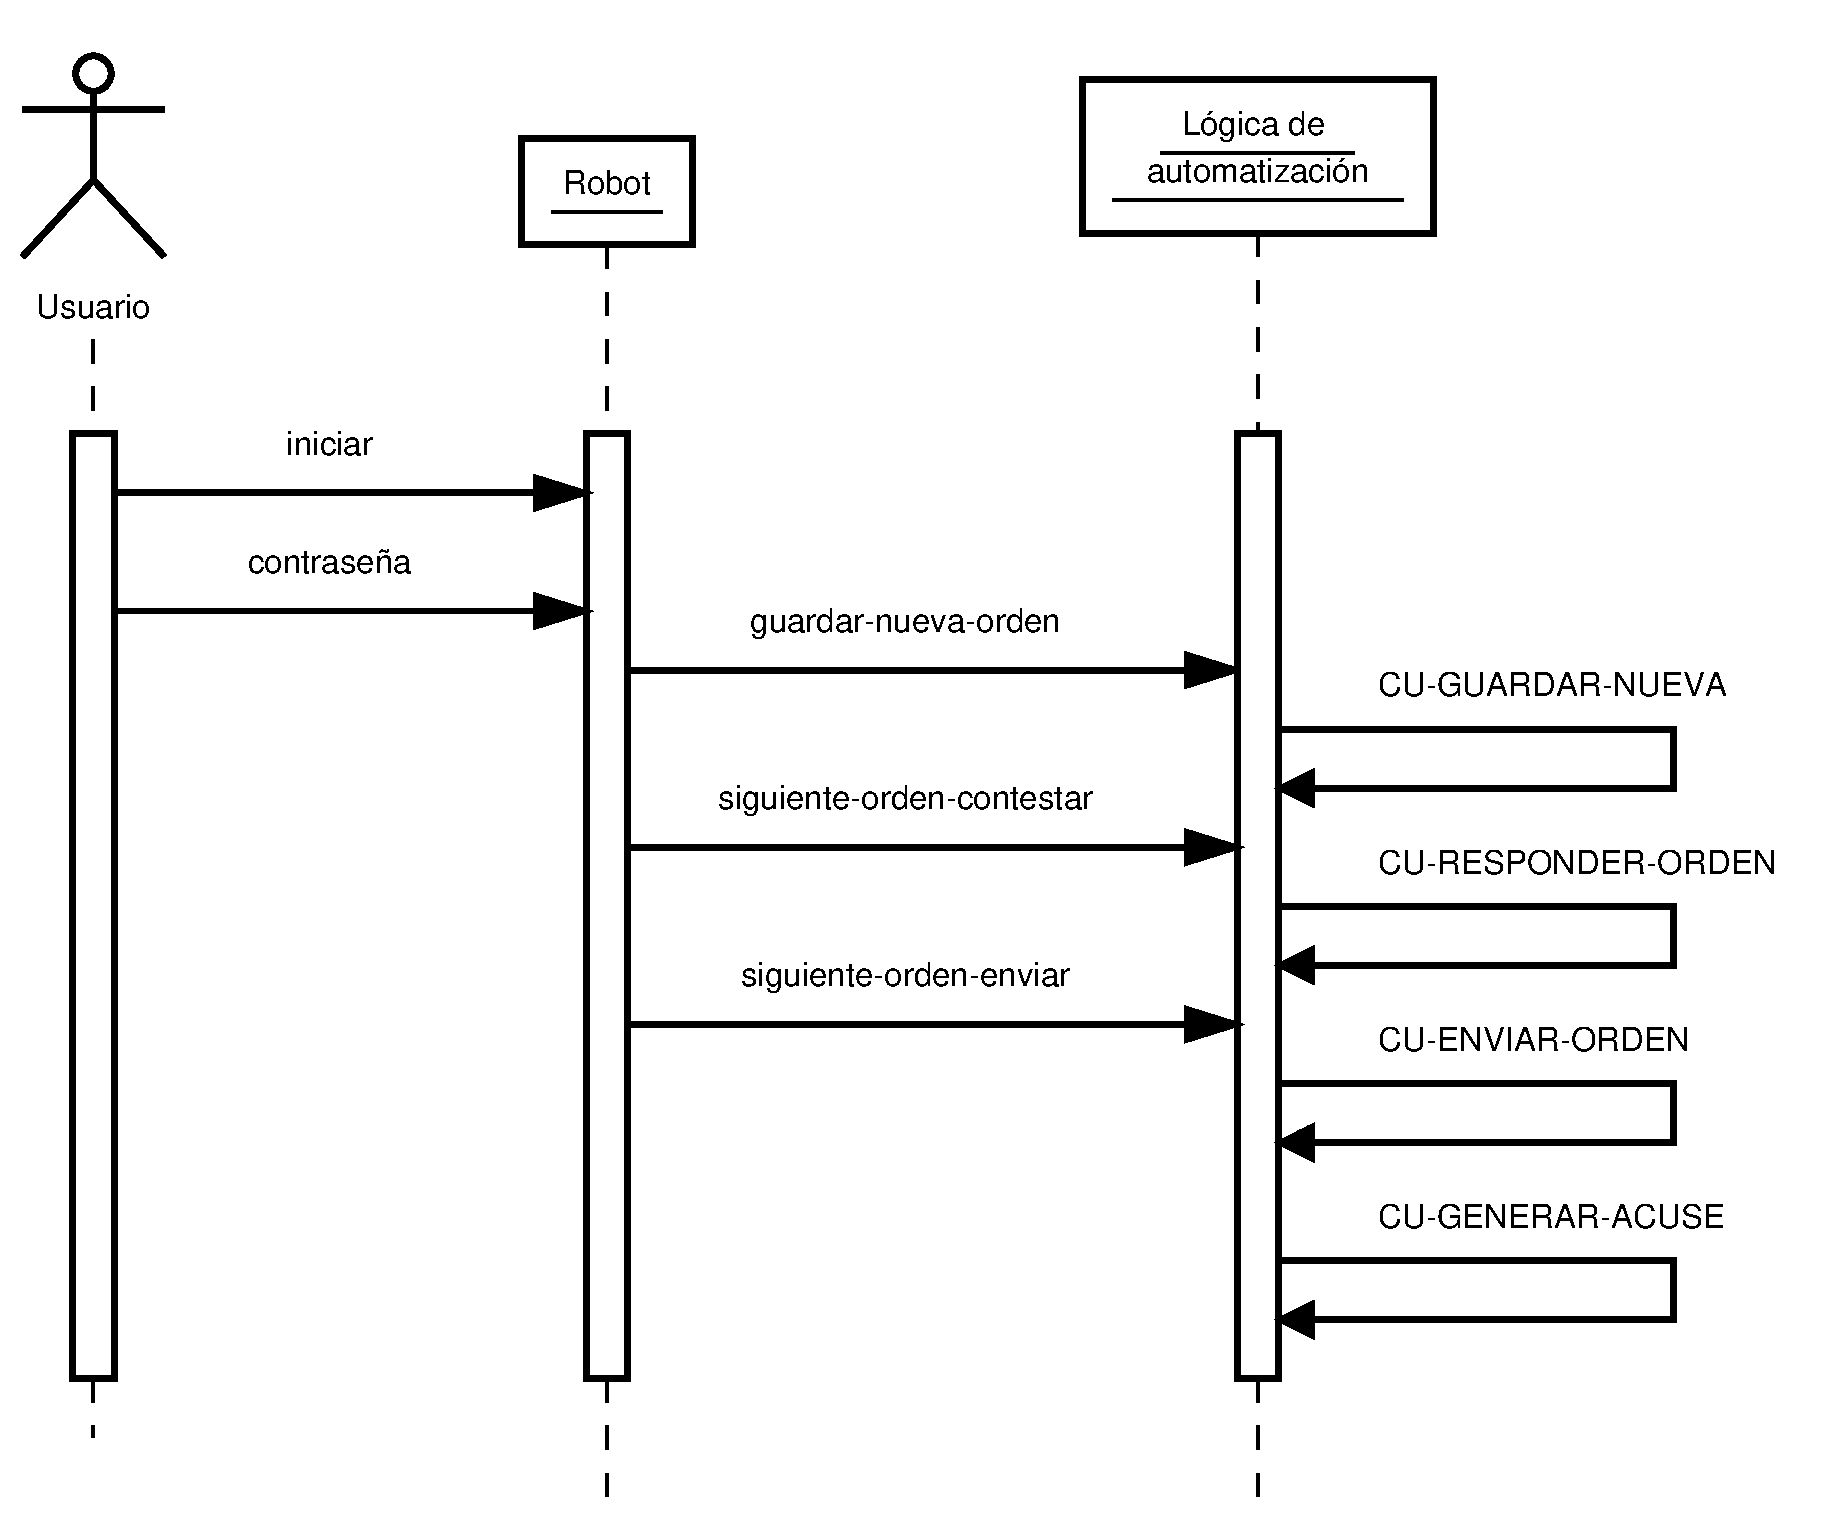
\includegraphics[scale=0.7]{dia-seq-cu-contestar}
	\caption{Diagrama de secuencia del caso de uso CU-CONTESTAR.}
	\label{fig:dia-seq-cu-contestar}
\end{figure}

\subsubsection{Guardar nueva orden}
El diseño para la solución del caso de uso \textbf{CU-GUARDAR-NUEVA} (sección \ref{cu-guardar-nueva}) utiliza los componentes \textbf{Agente}, \textbf{Lógica de Automatización} y \textbf{Persistencia}, tal solución se logra realizando las siguientes llamadas (En el diagrama de la Figura \ref{fig:dia-seq-cu-guardar-nueva} se muestra el diagrama de secuencia.):
\begin{enumerate}
	\item \textbf{Agente}: envía los datos de la nueva orden de reposición (mensaje 1 del diagrama).
	\item \textbf{Lógica de Automatización}: remueve (de encontrarse) los espacios en blanco al principio y al final de cada dato de la orden.
	\item \textbf{Lógica de Automatización}: construye la \textit{URL} de envío de la orden de reposición.
	\item \textbf{Lógica de Automatización}: envía la orden de reposición al componente de persistencia, (mensaje 2 del diagrama).
	\item \textbf{Persistencia}: almacena la orden de reposición en la base de datos.
\end{enumerate}

\begin{figure}[h]
	\centering
	\includegraphics[scale=0.7]{dia-seq-cu-guardar-nueva}
	\caption{Diagrama de secuencia del caso de uso CU-GUARDAR-NUEVA.}
	\label{fig:dia-seq-cu-guardar-nueva}
\end{figure}

\subsubsection{Responder orden}
El diseño para la solución del caso de uso \textbf{CU-RESPONDER-ORDEN} (sección \ref{cu-responder-orden}) utiliza los componentes \textbf{Agente}, \textbf{Lógica de Automatización} y \textbf{Persistencia}, tal solución se logra realizando las siguientes llamadas (En el diagrama de la Figura \ref{fig:dia-seq-cu-responder-orden} se muestra el diagrama de secuencia):
\begin{enumerate}
	\item \textbf{Agente}: pide la siguiente orden de reposición para contestar (mensaje 1 del diagrama).
	\item \textbf{Lógica de Automatización}: consulta el componente \textbf{Persistencia} para obtener la siguiente orden para contestar.
	\item \textbf{Persistencia}: obtiene la primera orden de reposición con estado \textbf{Nueva}.
	\item \textbf{Persistencia}: cambia el estado de la orden a \textbf{Siendo Contestada} (mensaje 3 del diagrama).
	\item \textbf{Agente}: pide los datos para llenar los formularios (mensaje 6 del diagrama).
	\item \textbf{Agente}: pide almacenar los datos de la orden de reposición contestada (mensaje 7 del diagrama).
	\item \textbf{Lógica de Automatización}: envía los datos de la orden contestada al componente \textbf{Persistencia} para que sean almacenados (mensaje 8 del diagrama).
	\item \textbf{Lógica de Automatización}: manda el cambio de estado de la orden a \textbf{Contestada} (mensaje 9 del diagrama).
\end{enumerate}

\begin{figure}[h]
	\centering
	\includegraphics[scale=0.7]{dia-seq-cu-responder-orden}
	\caption{Diagrama de secuencia del caso de uso CU-RESPONDER-ORDEN.}
	\label{fig:dia-seq-cu-responder-orden}
\end{figure}

\subsubsection{Enviar orden}
El diseño para la solución del caso de uso \textbf{CU-ENVIAR-ORDEN} (sección \ref{cu-enviar-orden}) utiliza los componentes \textbf{Agente}, \textbf{Lógica de Automatización} y \textbf{Persistencia}, tal solución se logra realizando las siguientes llamadas (En el diagrama de la Figura \ref{fig:dia-seq-cu-enviar-orden} se muestra el diagrama de secuencia):
\begin{enumerate}
	\item \textbf{Agente}: pide la siguiente orden de reposición para enviar (mensaje 1 del diagrama).
	\item \textbf{Lógica de Automatización}: consulta el componente \textbf{Persistencia} para obtener la siguiente orden para enviar (mensaje 2 del diagrama).
	\item \textbf{Persistencia}: obtiene la primera orden de reposición con estado \textbf{Contestada}.
	\item \textbf{Persistencia}: cambia el estado de la orden a \textbf{Siendo Enviada} (mensaje 3 del diagrama).
	\item \textbf{Agente}: dirige el explorador a la \textit{URL de envío}.
	\item \textbf{Agente}: manda almacenar el folio de envío (mensaje 6 del diagrama).
	\item \textbf{Lógica de Automatización}: utiliza el componente \textbf{Persistencia} para almacenar el folio de envío (mensaje 7 del diagrama).
	\item \textbf{Lógica de Automatización}: actualiza el estado de la orden a \textbf{Enviada} (mensaje 8 del diagrama).
\end{enumerate}

\begin{figure}[h]
	\centering
	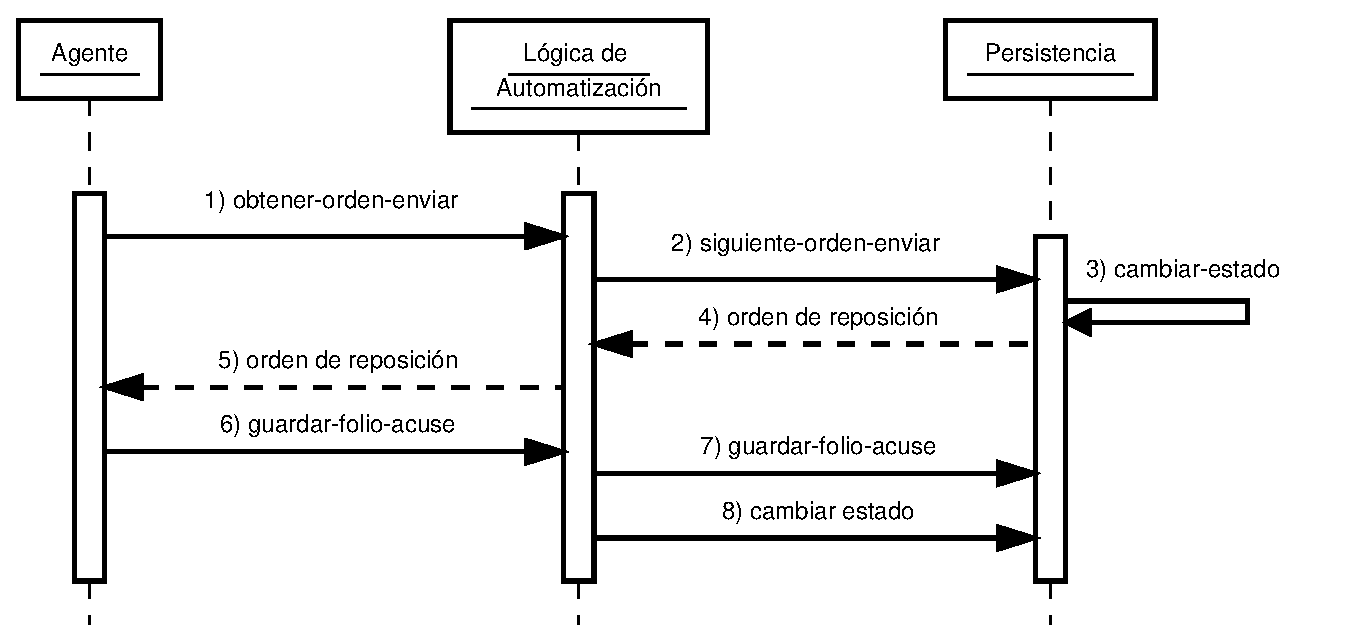
\includegraphics[scale=0.7]{dia-seq-cu-enviar-orden}
	\caption{Diagrama de secuencia del caso de uso CU-ENVIAR-ORDEN.}
	\label{fig:dia-seq-cu-enviar-orden}
\end{figure}

\subsubsection{Generar acuse de envío}
El diseño para la solución del caso de uso \textbf{CU-GENERAR-ACUSE} (sección \ref{cu-generar-acuse}) utiliza los componentes \textbf{Lógica de Automatización}, \textbf{Persistencia}, \textbf{Generador de Reportes} y \textbf{Sistema de Archivos} tal solución se logra realizando las siguientes llamadas (En el diagrama de la Figura \ref{fig:dia-seq-cu-generar-acuse} se muestra el diagrama de secuencia):
\begin{enumerate}
	\item \textbf{Lógica de Automatización}: pide los datos de la orden de reposición al componente \textbf{Persistencia} (mensaje 1 del diagrama).
	\item \textbf{Lógica de Automatización}: pide la generación del acuse de envío al componente \textbf{Generador de Reportes} (mensaje 2 del diagrama).
	\item \textbf{Generador de Reportes}: pide almacenar el acuse de envío al componente \textbf{Sistema de Archivos} (mensaje 3 del diagrama).
\end{enumerate}

\begin{figure}[h]
	\centering
	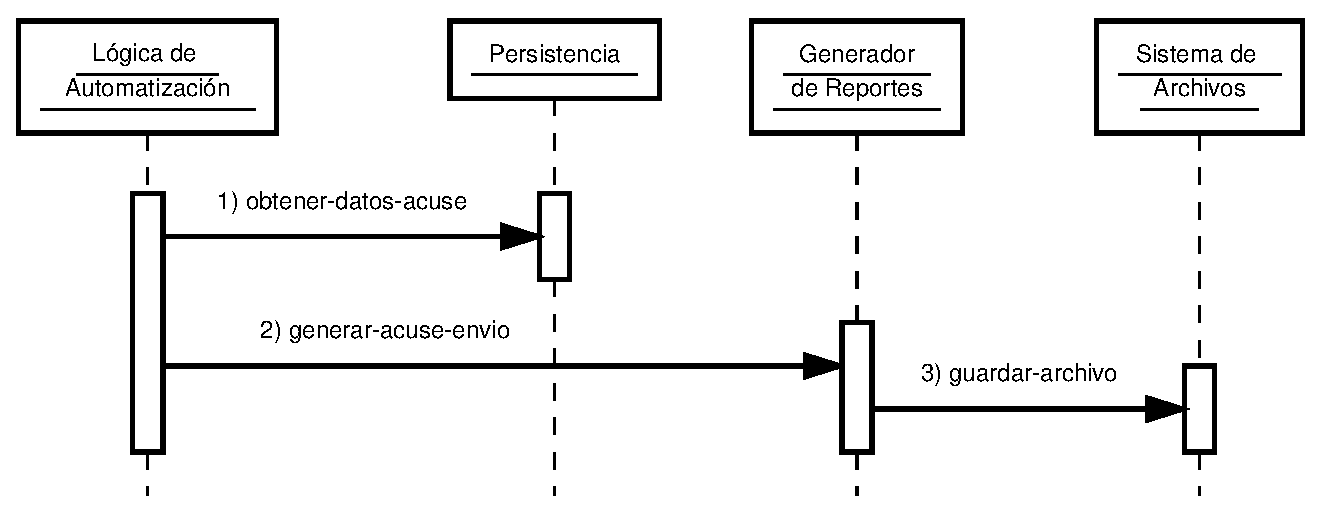
\includegraphics[scale=0.7]{dia-seq-cu-generar-acuse}
	\caption{Diagrama de secuencia del caso de uso CU-GENERAR-ACUSE.}
	\label{fig:dia-seq-cu-generar-acuse}
\end{figure}

\subsubsection{Verificar órdenes}
El diseño de la solución al caso de uso \textbf{CU-VERIFICAR} (sección \ref{cu-verificar}) se lleva a cabo entre el actor \textbf{Usuario} y los componentes \textbf{Agente} \textbf{Lógica de Automatización} tal solución se logra realizando las siguientes llamadas (En el diagrama de la Figura \ref{fig:dia-seq-cu-verificar} se muestra el diagrama de secuencia):
\begin{enumerate}
	\item \textbf{Usuario}: inicia la ejecución del agente (mensaje 1 del diagrama).
	\item \textbf{Agente}: dirige el explorador de Internet a la página del Sistema de Abastecimiento y pide al usuario la contraseña para ingresar.
	\item \textbf{Usuario}: proporciona la contraseña (mensaje 2 del diagrama).
	\item \textbf{Agente}: realiza el acceso al Sistema de Abastecimiento
	\item \textbf{Agente}: dirige el explorador de Internet a la búsqueda de órdenes de reposición.
	\item \textbf{Agente}: pide el rango de fechas al componente \textbf{Lógica de Automatización} (mensaje 3 del diagrama).
	\item \textbf{Agente}: realiza la búsqueda de órdenes de reposición \textit{canceladas}.
	\item \textbf{Agente}: envía el listado con los números de orden de reposición resultantes al componente \textbf{Lógica de Automatización} (mensaje 4 del diagrama).
	\item \textbf{Lógica de Automatización}: ejecuta los casos de uso \textbf{CU-ACTUALIZAR-ESTATUS-SA}(mensaje 5 del diagrama).
\end{enumerate}

\begin{figure}[h]
	\centering
	\includegraphics[scale=0.7]{dia-seq-cu-verificar}
	\caption{Diagrama de secuencia del caso de uso CU-VERIFICAR.}
	\label{fig:dia-seq-cu-verificar}
\end{figure}

\subsubsection{Actualizar estatus de Sistema de Abastecimiento}
El diseño para la solución del caso de uso \textbf{CU-ACTUALIZAR-ESTATUS-SA} (sección \ref{cu-actualizar-estatus-sa}) utiliza los componentes \textbf{Agente}, \textbf{Lógica de Automatización} y \textbf{Persistencia}, tal solución se logra realizando las siguientes llamadas (En el diagrama de la Figura \ref{fig:dia-seq-cu-actualizar-estatus-sa} se muestra el diagrama de secuencia):
\begin{enumerate}
	\item \textbf{Lógica de Automatización}: envía el listado de con los números de órdenes de reposición al componente \textbf{Persistencia} para actualizar en la base de datos el estado conocido en el Sistema de Abastecimiento (mensaje 1 del diagrama).
\end{enumerate}

\begin{figure}[h]
	\centering
	\includegraphics[scale=0.7]{dia-seq-cu-actualizar-estatus-sa}
	\caption{Diagrama de secuencia del caso de uso CU-ACTUALIZAR-ESTATUS-SA.}
	\label{fig:dia-seq-cu-actualizar-estatus-sa}
\end{figure}

\subsubsection{Entrar en interfaz Web}
El diseño de la solución al caso de uso \textbf{CU-ENTRAR-WEB} (sección \ref{cu-entrar-web}) se lleva a cabo entre el actor \textbf{Usuario} y los componentes \textbf{Portal Web} y \textbf{Persistencia} tal solución se logra realizando las siguientes llamadas (En el diagrama de la Figura \ref{fig:dia-seq-cu-entrar-web} se muestra el diagrama de secuencia):
\begin{enumerate}
	\item \textbf{Usuario}: introduce su nombre de usuario y contraseña \textbf{credenciales} (mensaje 1 del diagrama).
	\item \textbf{Portal Web}: envía el nombre de usuario al componente \textbf{Persistencia} que realiza la búsqueda de los datos del usuario (mensaje 2 del diagrama).
	\item \textbf{Portal Web}: compara la contraseña con la almacenada en la base de datos.
	\begin{enumerate}
		\item \textit{Si las credenciales son válidas}: el \textbf{Portal Web}regresa al \textbf{Usuario} un código de acceso temporal (mensaje 3 del diagrama).
		\item \textit{Si las credenciales son inválidas}: el \textbf{Portal Web}regresa al \textbf{Usuario} un mensaje de error (mensaje 4 del diagrama).
	\end{enumerate}
\end{enumerate}

\begin{figure}[h]
	\centering
	\includegraphics[scale=0.7]{dia-seq-cu-entrar-web}
	\caption{Diagrama de secuencia del caso de uso CU-ENTRAR-WEB.}
	\label{fig:dia-seq-cu-entrar-web}
\end{figure}

\subsubsection{Generar reporte}
El diseño de la solución al caso de uso \textbf{CU-GENERAR-REPORTE} (sección \ref{cu-generar-reporte}) se lleva a cabo entre el actor \textbf{Usuario} y los componentes \textbf{Portal Web}, \textbf{Persistencia}, \textbf{Generador de Reportes} y  \textbf{Sistema de Archivos} tal solución se logra realizando las siguientes llamadas (En el diagrama de la Figura \ref{fig:dia-seq-cu-generar-reporte} se muestra el diagrama de secuencia):
\begin{enumerate}
	\item \textbf{Usuario}: selecciona el tipo de reporte y el rango de fechas (mensaje 1 del diagrama).
	\item \textbf{Portal Web}: pide la búsqueda de órdenes al componente \textbf{Persistencia} (mensaje 2 del diagrama).
	\item \textbf{Portal Web}: envía las órdenes para generar el reporte (mensaje 3 del diagrama).
	\item \textbf{Generador de Reportes}: genera el reporte.
	\item \textbf{Generador de Reportes}: pide al componente \textbf{Sistema de Archivos} almacenar el reporte (mensaje 4 del diagrama).
	\item \textbf{Generador de Reportes}: regresa la ruta donde se guardó el componente (mensaje 5 del diagrama).
	\item \textbf{Portal Web}: muestra al \textbf{Usuario} la ruta donde se encuentra el reporte (mensaje 6 del diagrama).
\end{enumerate}

\begin{figure}[h]
	\centering
	\includegraphics[scale=0.7]{dia-seq-cu-generar-reporte}
	\caption{Diagrama de secuencia del caso de uso CU-GENERAR-REPORTE.}
	\label{fig:dia-seq-cu-generar-reporte}
\end{figure}

\subsubsection{Actualizar catálogo}
El diseño de la solución al caso de uso \textbf{CU-ACTUALIZAR-CATALOGO} (sección \ref{cu-actualizar-catalogo}) se lleva a cabo entre el actor \textbf{Usuario} y los componentes \textbf{Portal Web} y \textbf{Persistencia} tal solución se logra realizando las siguientes llamadas (En el diagrama de la Figura \ref{fig:dia-seq-cu-actualizar-catalogo} se muestra el diagrama de secuencia):
\begin{enumerate}
	\item \textbf{Usuario}: selecciona el catálogo y el archivo (mensaje 1 del diagrama).
	\item \textbf{Portal Web}: pide la actualización del catálogo al componente \textbf{Persistencia} (mensaje 2 del diagrama).
	\item \textbf{Portal Web}: muestra al \textbf{Usuario} la cantidad de registros almacenados (mensaje 3 del diagrama).
\end{enumerate}

\begin{figure}[h]
	\centering
	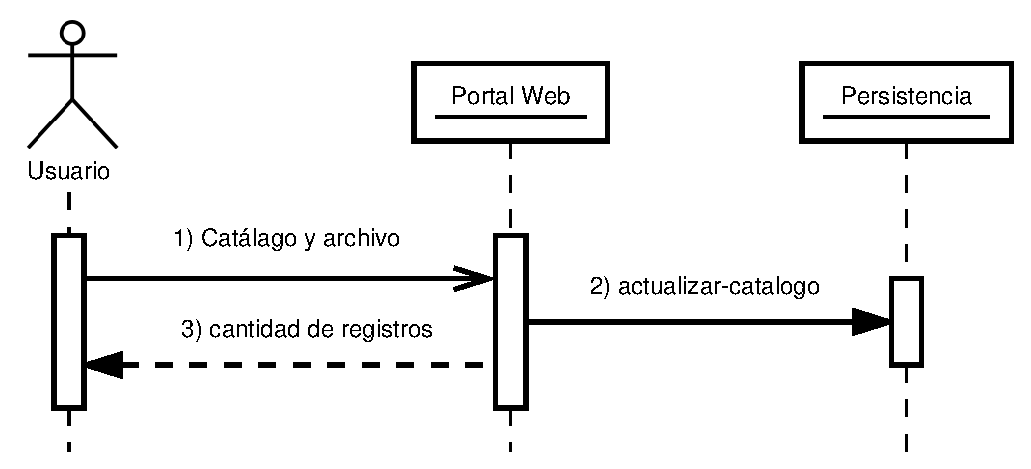
\includegraphics[scale=0.7]{dia-seq-cu-actualizar-catalogo}
	\caption{Diagrama de secuencia del caso de uso CU-ACTUALIZAR-CATALOGO.}
	\label{fig:dia-seq-cu-actualizar-catalogo}
\end{figure}

\subsubsection{Buscar órdenes}
El diseño de la solución al caso de uso \textbf{CU-BUSCAR} (sección \ref{cu-buscar}) se lleva a cabo entre el actor \textbf{Usuario} y los componentes \textbf{Portal Web} y \textbf{Persistencia} tal solución se logra realizando las siguientes llamadas (En el diagrama de la Figura \ref{fig:dia-seq-cu-buscar} se muestra el diagrama de secuencia):
\begin{enumerate}
	\item \textbf{Usuario}: llenada el formulario de búsqueda \textbf{filtro} (mensaje 1 del diagrama).
	\item \textbf{Portal Web}: pide la realización de la búsqueda de órdenes al componente \textbf{Persistencia} (mensaje 2 del diagrama).
	\item \textbf{Portal Web}: muestra al \textbf{Usuario} el listado de órdenes de reposición encontradas (mensaje 3 del diagrama).
\end{enumerate}

\begin{figure}[h]
	\centering
	\includegraphics[scale=0.7]{dia-seq-cu-buscar}
	\caption{Diagrama de secuencia del caso de uso CU-BUSCAR.}
	\label{fig:dia-seq-cu-buscar}
\end{figure}

\subsubsection{Visualizar orden}
El diseño de la solución al caso de uso \textbf{CU-VISUALIZAR} (sección \ref{cu-visualizar}) se lleva a cabo entre el actor \textbf{Usuario} y los componentes \textbf{Portal Web} y \textbf{Persistencia} tal solución se logra realizando las siguientes llamadas (En el diagrama de la Figura \ref{fig:dia-seq-cu-visualizar} se muestra el diagrama de secuencia):
\begin{enumerate}
	\item \textbf{Usuario}: selecciona la orden de reposición (mensaje 1 del diagrama).
	\item \textbf{Portal Web}: pide la realización de la búsqueda de la orden al componente \textbf{Persistencia} (mensaje 2 del diagrama).
	\item \textbf{Portal Web}: muestra al \textbf{Usuario} la información de la orden de reposición.
\end{enumerate}

\begin{figure}[h]
	\centering
	\includegraphics[scale=0.7]{dia-seq-cu-visualizar}
	\caption{Diagrama de secuencia del caso de uso CU-VISUALIZAR.}
	\label{fig:dia-seq-cu-visualizar}
\end{figure}

\subsubsection{Editar orden}
Ver sección \ref{cu-contestar}.\\
El diseño de la solución al caso de uso \textbf{CU-EDITAR} (sección \ref{cu-editar}) se lleva a cabo entre el actor \textbf{Usuario} y los componentes \textbf{Portal Web} y \textbf{Persistencia} tal solución se logra realizando las siguientes llamadas (En el diagrama de la Figura \ref{fig:dia-seq-cu-editar} se muestra el diagrama de secuencia):
\begin{enumerate}
	\item \textbf{Usuario}: activa la edición de la orden de reposición (mensaje 1 del diagrama).
	\item \textbf{Usuario}: modifica la información de la orden de reposición (mensaje 2).
	\item \textbf{Portal Web}: pide la actualización de la orden al componente \textbf{Persistencia} (mensaje 3 del diagrama).
\end{enumerate}

\begin{figure}[h]
	\centering
	\includegraphics[scale=0.7]{dia-seq-cu-editar}
	\caption{Diagrama de secuencia del caso de uso CU-EDITAR.}
	\label{fig:dia-seq-cu-editar}
\end{figure}


%===============================================================================
%===============================================================================

\newpage
\section{Diseño de la base de datos}
La base de datos tiene dos finalidades, guardar la información capturada de las órdenes de reposición atendidas así como los catálogos necesarios para los procesos automatizados y generación de reportes; la segunda es almacenar la información de los usuarios autorizados para utilizar el portal web.\\
El diseño de la base de datos se centra en los siguientes grupos\footnote{Los nombres de las tablas están escritos utilizando letras minúsculas de alfabeto inglés y guión bajo $([a-z]{\textunderscore})^+$}(ver Figura \ref{fig:dia-er-resumen}):
\begin{enumerate}
	\item Tablas de las órdenes de reposición.
	\item Tablas del registro de eventos.
	\item Tablas de los usuarios de la interfaz web.
	\item Catálogos para generación de reportes.
\end{enumerate}
\begin{figure}[h]
  \centering
  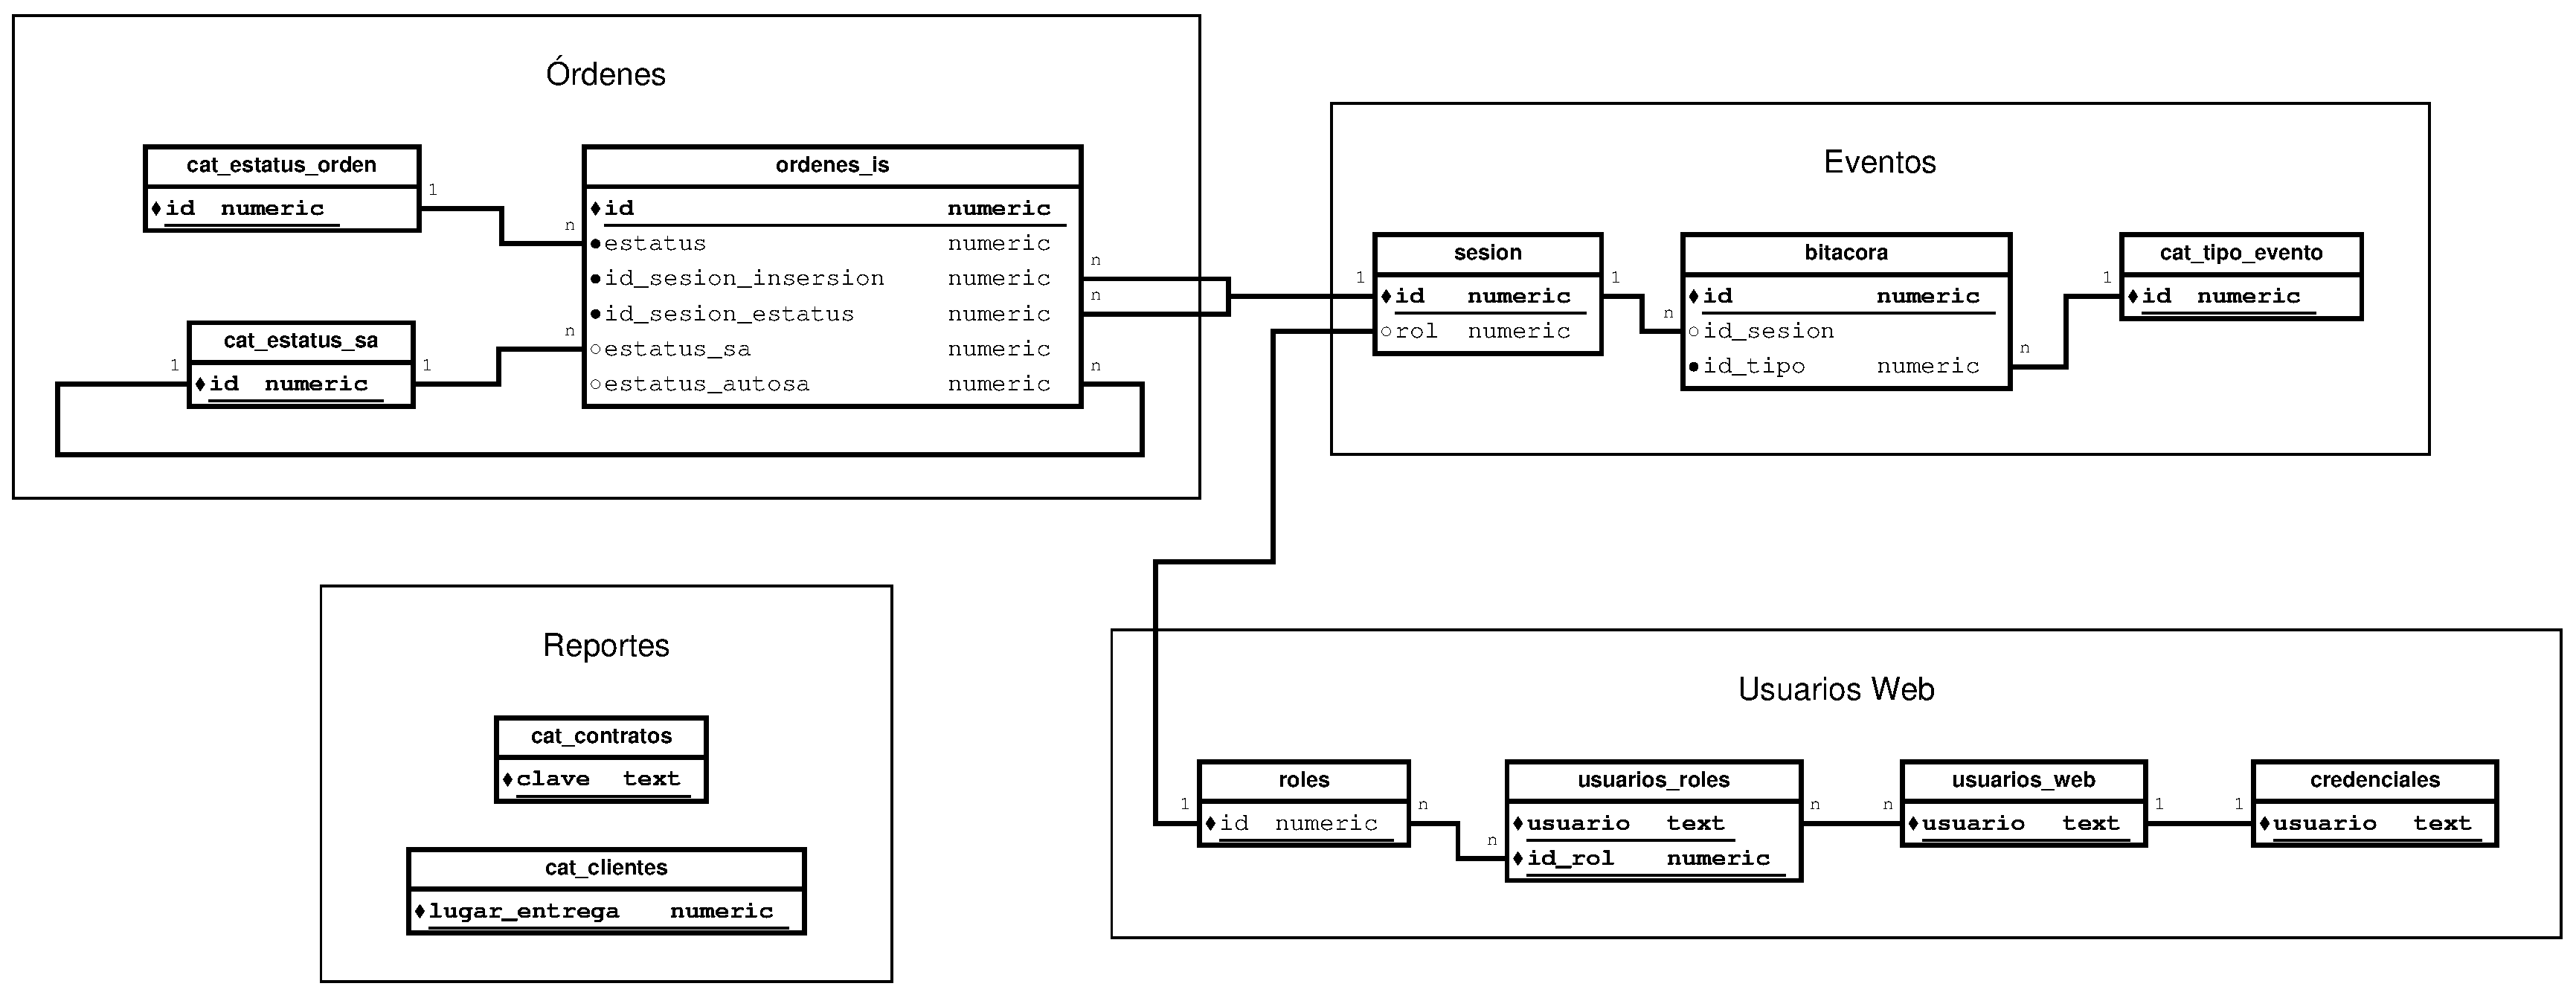
\includegraphics[width=\textwidth]{dia-er-resumen}
  \caption{Diagrama Entidad Relación de el Sistema AutoSA.}
  \label{fig:dia-er-resumen}
\end{figure}


\subsection{Tablas de las órdenes de reposición}
En estas tablas (ver Figura \ref{fig:dia-er-ordenes}) se almacenan las órdenes de reposición atendidas durante la rutina automatizada para responder órdenes de reposición en el Sistema de Abastecimiento\footnote{Ver caso de uso \ref{cu-contestar}}, de igual manera también es utilizada en la verificación de órdenes de reposición canceladas\footnote{Ver caso de uso \ref{cu-verificar}}.
\begin{figure}[h]
  \centering
  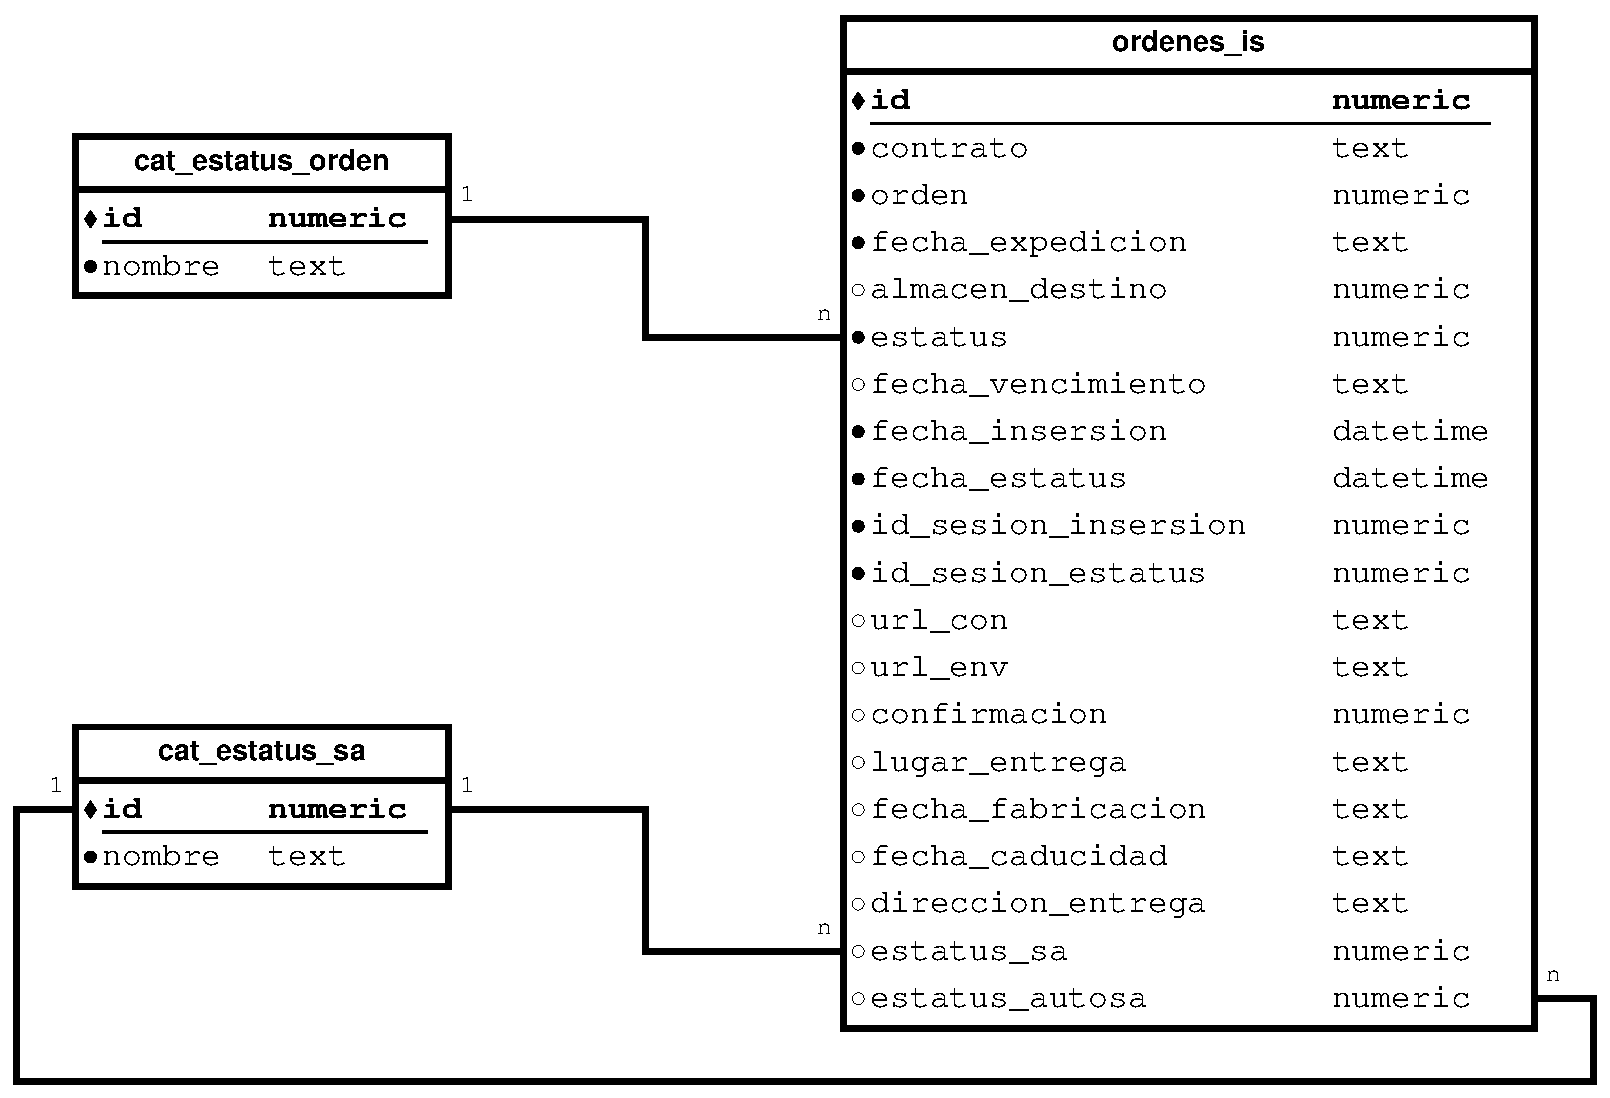
\includegraphics[scale=0.5]{dia-er-ordenes} 
  \caption{Diagrama Entidad Relación para el registro de órdenes de reposición.}
  \label{fig:dia-er-ordenes}
\end{figure}
\paragraph{ordenes{\textunderscore}is:} Contiene el registro de las órdenes de reposición del Sistema de Abastecimiento que han sido atendidas por la rutina de automatización.
\paragraph{cat{\textunderscore}estatus{\textunderscore}orden:} Este catálogo no debe ser alterado, contiene los posibles estatus que pude tomar una orden durante el ciclo de vida de la aplicación.
\paragraph{cat{\textunderscore}estatus{\textunderscore}sa:} Este catálogo contiene los estados definidos por el Sistema de Abastecimiento para registrar y almacenar una orden de reposición.


\subsection{Tablas del registro de eventos}
El registro de eventos es todo lo relacionado con actividad de los actores del sistema (agentes de automatización y usuarios), como se muestra en la Figura \ref{fig:dia-er-bitacora}.
\begin{figure}[h]
  \centering
  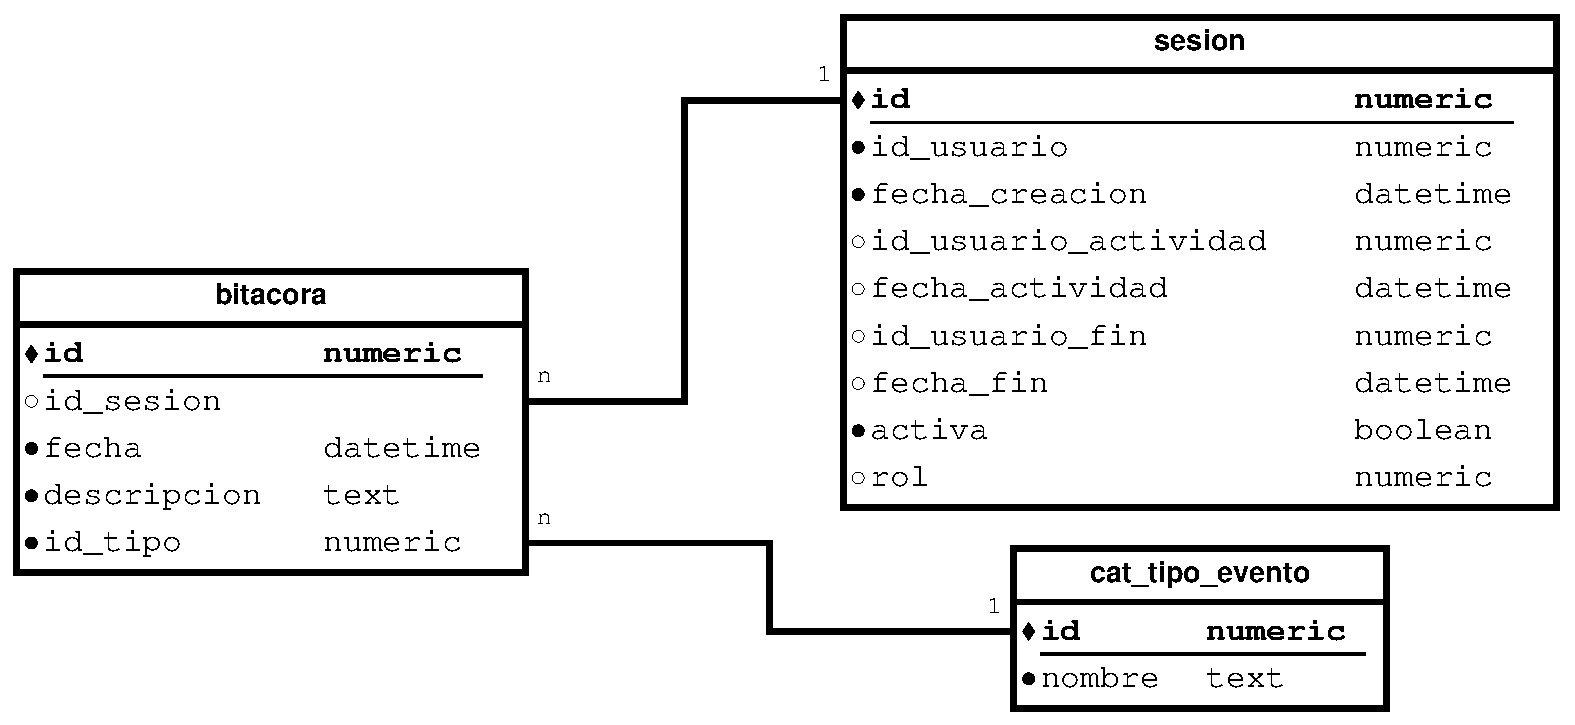
\includegraphics[scale=0.5]{dia-er-bitacora} 
  \caption{Diagrama Entidad Relación para el registro de eventos.}
  \label{fig:dia-er-bitacora}
\end{figure}
\paragraph{bitacora:} Lleva el registro de eventos ocurridos durante la ejecución de las rutinas de automatización, el evento puede estar ligado a una sesión.
\paragraph{cat{\textunderscore}tipo{\textunderscore}evento:} Catálogo con los tipos de eventos que pueden ser registrados en la bitácora.
\paragraph{sesion:} Define una sesión bajo la cual se ejecuta una rutina de automatización, la sesión puede definir implícitamente un usuario y un rol.


\subsection{Tablas de los usuarios de la interfaz web}
Las tablas de este grupo son utilizadas para gestionar el acceso a la interfaz web\footnote{Ver caso de uso \ref{cu-entrar-web}} (ver Figura \ref{fig:dia-er-web}).
\begin{figure}[h]
  \centering
  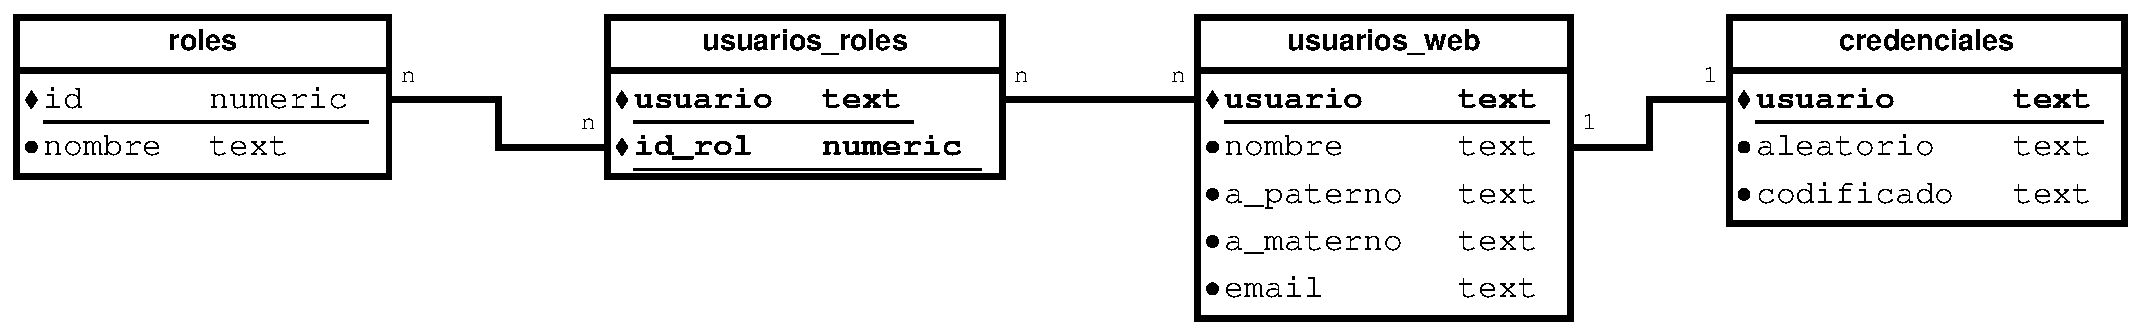
\includegraphics[scale=0.5]{dia-er-web} 
  \caption{Diagrama Entidad Relación para el manejo de usuarios.}
  \label{fig:dia-er-web}
\end{figure}
\paragraph{roles:}Contiene los roles (permisos) que los usuarios pueden tener en la interfaz web.
\paragraph{sesion:}Contiene información de las sesiones de los usuarios de la interfaz web.
\paragraph{usuarios{\textunderscore}web:} Contiene la información de los usuarios de la interfaz web.
\paragraph{credenciales:} Contiene la credenciales con las cuales los usuarios autentican su acceso a la interfaz web.


\subsection{Catálogos para la generación de reportes}
Estas tablas contienen catálogos (ver Figura \ref{fig:dia-er-reportes}) que son necesarios para la generación de los reportes\footnote{Ver casos de uso \ref{cu-generar-reporte} y \ref{cu-actualizar-catalogo}} que sirven que las siguientes áreas de la farmacéutica continúen con la atención de las órdenes de reposición.
\begin{figure}[h]
  \centering
  \includegraphics[scale=0.5]{dia-er-reportes} 
  \caption{Diagrama Entidad Relación de los catálogos para la generación de vistas.}
  \label{fig:dia-er-reportes}
\end{figure}
\paragraph{cat{\textunderscore}clientes:} Este catálogo contiene información sobre la localización física de los lugares donde deben ser entregados los productos.
\paragraph{cat{\textunderscore}contratos:} Este catálogo contiene información referente a acuerdos comerciales referentes a los productos requeridos en las órdenes de reposición.


\section{Resumen}
En este capítulo se ha mostrado la arquitectura del Sistema AutoSA, los componentes del mismo y las interfaces que ofrecen. Posteriormente se ha mostrado el flujo de mensajes entre los componentes del sistema para llevar a cabo los casos de uso del Capítulo \ref{cap2}. Así mismo se ha modelado la base de datos que a grandes rasgos está destinada a almacenar información de las órdenes de reposición e información de los usuarios del Sistema AutoSA.\\
El diseño planteado será implementado en el siguiente capítulo donde se verá a detalle el funcionamiento de cada módulo así como algoritmos, tecnologías y marcos de trabajo utilizados. 

\chapter{Implementación}\label{cap4}

\section{Tecnologías utilizadas}
\subsection{Base de datos relacional}\label{sec-bd-r}
Una base de datos relaciones es una colección de tablas relacionadas entre sí. La colección de tablas se describe a sí misma en cuanto a que el significado de los datos contenidos pertenecen a un mismo ámbito\cite{DataBaseConcepts}.\\
Una base de datos es administrada mediante un Sistema Administrador de Bases de Datos (DBMS por sus siglas en inglés), un DBMS es un programa de computadora usado para crear, procesas y administrar bases de datos. El DBMS recibe peticiones en lenguaje SQL (como se describe más adelante) y traduce esas peticiones a acciones dentro de la base de datos\cite{DataBaseConcepts}.\\
Para el desarrollo del proyecto AutoSA se han ocupado los siguientes conceptos:
\begin{enumerate}
	\item \textbf{Tabla}: una tabla es un conjunto de renglones (registros) y columnas (atributos) que cumple con las siguientes características\cite{DataBaseConcepts}:
	\begin{enumerate}
		\item Los renglones contienen unicamente datos relacionados con la tabla.
		\item Las entradas de una columna contienen un solo valor.
		\item Todas las entradas de una columna son del mismo tipo.
		\item Las columnas tienen un nombre único dentro de la tabla.
		\item El orden de las columnas y los renglones no es relevante.
		\item No contiene dos renglones idénticos.
	\end{enumerate}
	\item \textbf{Vista}: es una tabla derivada de una consulta de otras tablas, estas tablas pueden ser tablas de la base de datos o vistas definidas previamente. Una vista es considerada como tabla virtual porque no necesariamente existe físicamente a diferencia de una tabla de la base cuyas tuplas siempre están almacenadas físicamente en la base de datos\cite{FundamentalsOfDBSystems}.
	\item \textbf{Llave primaria}: es el conjunto de columnas que identifican de manera unívoca a cada renglón de la tabla.\cite{DataBaseConcepts}
	\item \textbf{Llave foránea}: define la relación de una tabla, \textbf{A}, hacia otra \textbf{B} y satisface las siguientes condiciones\cite{FundamentalsOfDBSystems, DataBaseConcepts}:
	\begin{enumerate}
		\item Los atributos de las tablas \textbf{A} y \textbf{B} son del mismo tipo y se corresponden uno a uno.
		\item Los atributos en la tabla \textbf{B} son exactamente los mismos de la llave primaria de la tabla \textbf{B}.
	\end{enumerate}
	\item \textbf{Restricción $NOT$ $NULL$}: indica que el valor del atributo no puede ser nulo\cite{FundamentosSistemasBasesDatos}. 
	\item \textbf{Índice}: es una estructura auxiliar para agilizar la obtención de registros. Los índices proveen rutas de acceso alternativo a los registros de la base de datos sin afectar la colocación física de los registros\cite{FundamentalsOfDBSystems}.
	\item \textbf{Lenguaje Estructurado de Consulta}\label{sec-sql}: del inglés Structured Query Language (SQL), fue desarrollado por IBM\textsuperscript{\textcopyright} al final de los años 70, es un lenguaje de datos orientado a texto, ha sido avalado por el Instituto Nacional de Estándares Americanos (ANSI por sus siglas en inglés) dando así los estándares ANSI para SQL, principalmente para este trabajo el estándar ANSI-92 o SQL-92.
	\item \textbf{Lenguaje de Definición de Datos}: DDL por sus siglas en inglés, es un lenguaje de SQL cuya función es describir la creación de estructuras tales como tablas, índices y restricciones, entre otras\cite{DataBaseConcepts}.
	\item \textbf{Lenguaje de Modelado de Datos}: DML por sus siglas en inglés, es un lenguaje de SQL cuya función es describir la modificación de datos, es decir, sentencias de inserción, borrado y actualización de datos\cite{DataBaseConcepts}.  
\end{enumerate}

\subsection{Java}\label{sec-java}

El lenguaje de programación Java fue creado en 1991 por James Gosling, Patrick Naughton, Chris Warth, Ed Frank y Mike Sheridan en 1991 bajo el nombre ``Oak'' y en 1995 cambiaron el nombre a Java. El lenguaje Java está basado en los lenguajes de programación C, de donde deriva su sintaxis y de C++, que se toma como base para las características del paradigma orientado a objetos. Java es un lenguaje orientado a objetos, estáticamente tipado y multiplataforma\cite{JavaCompleteReference, WellGroundedJavaDeveloper}.\\
El concepto de Java tiene varios componentes, para efectos de este proyecto se mencionarán los siguientes\cite{JavaCompleteReference, WellGroundedJavaDeveloper}:
\begin{enumerate}
	\item Lenguaje de programación Java: previamente descrito, es un lenguaje multiplataforma, estáticamente tipado y orientado a objetos.
	\item Máquina Virtual de Java: JVM por sus siglas en inglés, es el sistema de ejecución en tiempo real de Java\footnote{\textcolor{red}{Karla, \textbf{Sistem de ejecución en tiempo real de Java} fue lo que me pareció más correcto para traducir ``Java run-time system'' ¿qué opinas, sabes una traducción mejor?}}.
	\item Bytecode: es el nombre que recibe el conjunto optimizado de instrucciones diseñadas para ser ejecutadas en la JVM.
	\item Paquete de Desarrollo de Java JDK (Java Development Kit): es el conjunto de herramientas utilizadas para el desarrollo de software para la máquina virtual de Java.
	\item Ambiente de Ejecución de Java JRE (Java Runtime Environment): es la herramienta encargada de la creación y administración de instancias de la máquina virtual de Java.
\end{enumerate}

\subsection{Javascript}\label{sec-javascript}
\textcolor{blue}{Javascript es un lenguaje que lo único que tiene similar a Java es la sintaxis, y no mucho, así que por favor dejen de tratarlos como sinónimos (odio a los PMs)}\footnote{se recomienda no hacer mucho caso, escribí algo de Javascript nada más para tener texto en la sección.}.


\subsection{Sahi}\label{sec-sahi}
La compañía Sahi Pro\textsuperscript{\textcopyright}\cite{SahiPro} describe a su producto del mismo nombre como:
\begin{quote}
	Sahi es una herramienta enfocada a la automatización de pruebas para servicios Web, plataformas Web, móviles, escritorio de Windows\textsuperscript{\textcopyright} y ambientes de Java.
\end{quote}

Sahi incluye un modo de operación que permite ejecutar rutinas automatizadas sobre exploradores de Internet, la forma en Sahi logra la ejecución de rutinas es actuando como proxy\footnote{Un proxy es un intermediario entre el cliente (explorador) y el servidor (página Web)\cite{BeginningUbuntuLinux}} entre el sitio Web y el explorador de Internet como se muestra en la Figura \ref{fig:dia-sahi-arq}. Cada vez que el explorador hace una petición al sitio Web, Sahi intercepta la comunicación e inserta código de Javascript que ejecuta la rutina automatizada.\cite{WebEng9IntConf, SahiPro}

\begin{figure}[h]
\centering
\includegraphics[width=\textwidth]{dia-sahi-arq}
\caption{Diagrama de flujo de Sahi\cite{SahiPro}.}
\label{fig:dia-sahi-arq}
\end{figure}

%\subsubsection{Java Data Base Controller}
%\subsubsection{Java IO}
%\subsubsection{Java Enterprise Edition}
%\subsection{Javascript}
%\subsection{Sahi}
%\subsection{iBatis}
%\subsection{Spring}
%\subsubsection{Spring MVC}
%\subsubsection{Spring JPA}
%\subsubsection{Spring Security}


\section{Implementación de base de datos}
El sistema AutoSA utiliza una base de datos relacional\footnote{Por confidencialidad no se hace mención específica del nombre y versión del sistema administrador de bases de datos.}(ver sección \ref{sec-bd-r}) para almacenar la información requerida en los casos de uso (ver sección \ref{sec:casos-uso}).\\
La implementación de la base de datos se ve reflejada en las rutinas con sentencias SQL (ver sección \ref{sec-bd-r}) donde se definen los objetos de la base de datos, tales rutinas se separan en dos grupos, las rutinas DDL y las rutinas DML.

\subsection{Rutinas de definición de datos}
Estas rutinas contienen las sentencias DDL (ver sección \ref{sec-bd-r}) para la creación de tablas, llaves primarias, llaves foráneas, índices y restricciones. En el código \ref{lst:sql-create-table} se muestra un ejemplo de la creación de una tabla.
\begin{lstlisting}[language=SQL, caption={Sentencia para crear una tabla.}, label={lst:sql-create-table}]
CREATE TABLE ordenes_is(
   id numeric(20,0) PRIMARY KEY NOT NULL,
   orden numeric(20,0) NOT NULL,
   estatus numeric(2,0) NOT NULL,
   id_sesion_insersion numeric(20,0) NOT NULL,
   id_sesion_estatus numeric(20,0) NOT NULL,
   estatus_sa numeric(2,0),
   estatus_sap numeric(2,0)
);
\end{lstlisting}

La generación de reportes que se menciona en el caso de uso \textbf{Generar reporte} (ver sección \ref{cu-generar-reporte}), utiliza una vista para la definición de la consulta de los datos del reporte (ver código \ref{lst:sql-create-view}, además se han implementado índices para agilizar tales consultas (ver código \ref{lst:sql-create-index}).

\begin{lstlisting}[language=SQL, caption={Sentencia para crear una vista.}, label={lst:sql-create-view}]
CREATE VIEW ordenes_contestadas AS
     SELECT *
       FROM ordenes_is
      WHERE id_sesion_estatus = :sesion
        AND estatus = 3
\end{lstlisting}

\begin{lstlisting}[language=SQL, caption={Sentencia para crear un índice.}, label={lst:sql-create-index}]
CREATE INDEX ordenes_contetadas_idx ON ordenes_is(id_sesion_estatus, estatus);
\end{lstlisting}

\subsection{Rutinas de modelado de datos}
Estas rutinas contienen la sentencias DML (ver sección \ref{sec-bd-r}) para insertar la información necesaria para la ejecución del sistema, como son, por ejemplo, los estados posibles de las órdenes de reposición (ver Figura \ref{fig:dia-estados-orden}), en el código \ref{lst:sql-insert} se muestra un ejemplo de la sentencia DML para insertar un registro.

\begin{lstlisting}[language=SQL, caption={Sentencia insertar un registro.}, label={lst:sql-insert}]
INSERT INTO cat_estatus_orden (id,nombre) VALUES (1,'NUEVA');
\end{lstlisting}

%================================================================================
%
%================================================================================

\section{Implementación de los componentes}

\subsection{Agente}
La implementación del componente Agente esta escrita en rutinas de Sahi (ver sección \ref{sec-sahi}), primero se mostrarán los puntos relevantes en la implementación de las rutinas de respuesta y envío de órdenes de reposición para después señalar como se realizar la ejecución mediante la herramienta gráfica de Sahi.

\subsubsection{Rutina para automatizar la respuesta de órdenes de reposición}\label{sec-aut-contestar}
La rutina para automatizar la respuesta de órdenes de reposición refleja el caso de uso  CU-CONTESTAR que se describe en la sección \ref{cu-contestar}, a continuación se muestran las secciones de código más relevantes de la rutina que realizan la ejecución del caso de uso citado así como los subsecuentes (ver diagrama en la Figura \ref{fig:dia-casos-uso}). Los puntos relevantes en la implementación de la rutina son los siguientes:
\begin{enumerate}
	\item Ingresar al Sistema de Abastecimiento, en el código \ref{lst:sah-session} se muestra la rutina para iniciar sesión en el Sistema de Abastecimiento:
	\begin{enumerate}
		\item Las líneas 1 y 2 se llenan los campos de usuario y contraseña.
		\item La línea 3 se envía el formulario.
		\item La línea 4 redirige a la pantalla con el listado de órdenes de reposición.  
	\end{enumerate}
	\begin{lstlisting}[language=Javascript, caption={Inicio de sesión en el Sistema de Abastecimiento.}, label={lst:sah-session}]
_setValue(_textbox("Usuario[1]"), $user);
_setValue(_password("Contras[1]"), $pwd);
_click(_submit("Ingresar al Sistema"));
_click(_image("Normal[2]"));
	\end{lstlisting}

	\item Recolectar las órdenes de reposición listadas, el código \ref{lst:sah-save-news} muestra un resumen de la automatización para guardar el listado de ordenes de reposición (ver caso de uso en la sección \ref{cu-guardar-nueva}):
	\begin{enumerate}
		\item La línea 1 muestra la declaración del ciclo para recorrer el listado de órdenes de reposición.
		\item Las líneas 2 a 4 muestran como se extrae el valor de los datos de una orden de reposición.
		\item Las líneas 5 a 8 muestran la obtención de las URLs para contestar y enviar las órdenes de reposición.
		\item La línea 9 es el almacenamiento de la nueva orden de reposición. 
	\end{enumerate}
	\begin{lstlisting}[language=Javascript, caption={Guardar lista de órdenes de reposición.}, label={lst:sah-save-news}]
for(var $i = 1 + $errores; $i <= $rowCount; $i++){
	var $contrato = _getText(_table(1).rows[$i].cells[0]);
	var $solicitud = _getText(_table(1).rows[$i].cells[1]);
	var $numorden = _getText(_table(1).rows[$i].cells[2]);
	var $urlcon = "";
	_log(_table(1).rows[$i].cells[6].childNodes[0].href);
	_set($urlcon, _table(1).rows[$i].cells[6].childNodes[0].href);
	var $urlenv = $urlcon.replace("respoOra", "enviaOra");
	var $inserted = $persistence.insertOrden($contrato, $solicitud, $numorden, $expedicion, $almacen, $urlcon, $urlenv, $idSesion);
}
	\end{lstlisting}

	\item Contestar una a una cada orden de reposición, el código \ref{lst:sah-respond} muestra un resumen de la automatización para contestar una orden de reposición (ver caso de uso en la sección \ref{cu-responder-orden}):
	\begin{enumerate}
		\item Las líneas 1 y 2 muestran como se redirige al explorador a la URL para contestar la orden de reposición.
		\item  Las líneas 3 muestran como se estable un valor en el formulario para contestar la orden de reposición.
		\item La línea 4 realiza el envío del formulario.
		\item La línea 5 manda la actualización de la orden de reposición en la base de datos.
	\end{enumerate}
	\begin{lstlisting}[language=Javascript, caption={Responder orden de reposición.}, label={lst:sah-respond}]
var $url = $entidad.getUrlCon();
_navigateTo($url);
_setValue(_textbox("Lote"), "SL");
_click(_submit("Agregar Captura"));
$logica.updateCantidad($contrato, $numorden, $cantidad, $idSesion);
	\end{lstlisting}

	\item Enviar las órdenes de reposición contestadas, el código \ref{lst:sah-send} muestra un resumen de la automatización para envíar una órden de reposición (ver caso de uso en la sección \ref{cu-enviar-orden}):
	\begin{enumerate}
		\item Las líneas 1 y 2 muestran como se redirige al explorador a la URL para enviar la orden de reposición.
		\item La líneas 3 a 6 crea un mapa con los datos de la orden de reposición.
		\item La línea 7 actualiza la orden de reposición en la base de datos. 
	\end{enumerate}
	\begin{lstlisting}[language=Javascript, caption={Enviar orden de reposición.}, label={lst:sah-send}]
var $url = $entidad.getUrlEnv();
_navigateTo($url);
$mapa = new java.util.LinkedHashMap();
for(var $llave in $orden){
	$mapa.put($llave, $orden[$llave]);
}
$logica.updateOrdenImss($mapa, $idSesion);
	\end{lstlisting}
\end{enumerate}

\subsubsection{Rutina para automatizar la verificación de órdenes de reposición canceladas}
La rutina para automatizar la verificación de órdenes de reposición canceladas refleja el caso de uso  CU-VERIFICAR que se describe en la sección \ref{cu-verificar}, a continuación se muestran las secciones de código más relevantes de la rutina que realizan la ejecución del caso de uso citado así como los subsecuentes (ver diagrama en la Figura \ref{fig:dia-casos-uso}). Los puntos relevantes en la implementación de la rutina son los siguientes:
\begin{enumerate}
	\item Ingresar al Sistema de Abastecimiento, el ingreso al sistema es idéntico a la rutina mostrada en la sección anterior (sección \ref{sec-aut-contestar}).

	\item Establecer los criterios de búsqueda, el código \ref{lst:sah-search} muestra un resumen de la automatización para :
	\begin{enumerate}
		\item La línea 1 muestra la consulta de las fechas que acotan la búsqueda.
		\item Las líneas 2 a 5 realizan la búsqueda en el Sistema de Abastecimiento.
		\item Las líneas 6 y 7 extraen la información de las órdenes de reposición que muestra el Sistema de Abastecimiento como resultado de la búsqueda.
		\item Las líneas 8 y 9 utilizan el componente \textbf{Lógica de automatización} para actualizar en la base de datos el estado de las órdenes de reposición canceladas.
	\end{enumerate}
	\begin{lstlisting}[language=Javascript, caption={Responder orden de reposición.}, label={lst:sah-search}]
$dateLimits = $logica.getDateLimits('dd/MM/yyyy');
_setSelected(_select("OrdStt"), "Canceladas");
_setValue(_textbox("OrdFeD"), $dateLimits[0]);
_setValue(_textbox("OrdFeA"), $dateLimits[1]);
_click(_submit(0));
var $html = '';
_set($html, _table(5).innerHTML);
$estado = $logica.getCancelStatus();
$logica.setSaiStatus($html, $estado, $idSesion);
	\end{lstlisting}
\end{enumerate}

\subsubsection{Ejecución de las rutinas de automatización}
La ejecución de las rutinas de sahi corresponden a los casos de uso CU-CONTESTAAR y 
CU-VERIFICAR (ver secciones \ref{cu-contestar} y \ref{cu-verificar} respectivamente), en ambos casos la ejecucuión es  
dejando la ejecución al usuario por medio de la interfaz gráfica de Sahi:
\begin{itemize}
	\item Iniciar Sahi sobre el explorar de Internet (ver Figura \ref{fig:ss-sahi-dashboard})
	\begin{figure}[h]
	\centering
	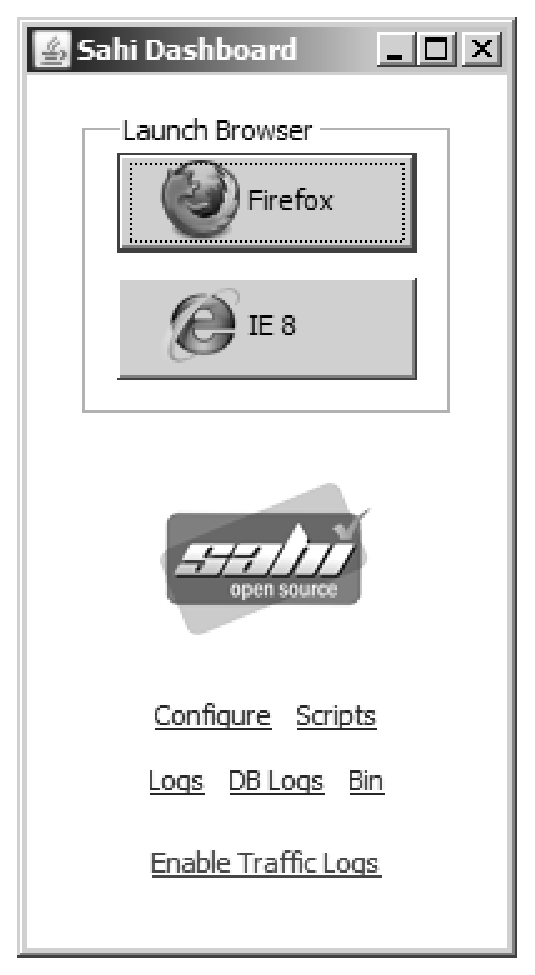
\includegraphics[scale=0.6]{ss-sahi-dashboard}
	\caption{Dashboard de Sahi.}
	\label{fig:ss-sahi-dashboard}
	\end{figure}

	\item Iniciar el controlador de Sahi y hacer los siguientes pasos (ver Figura \ref{fig:ss-sahi-controller}):
	\begin{enumerate}
		\item Seleccionar la rutina automatizada (contestar órdenes de reposición o verificación de órdenes de reposición)
		\item Ingresar la URL del Sistema de Abastecimiento
		\item Iniciar la ejecución.
	\end{enumerate}
	\begin{figure}[h]
	\centering
	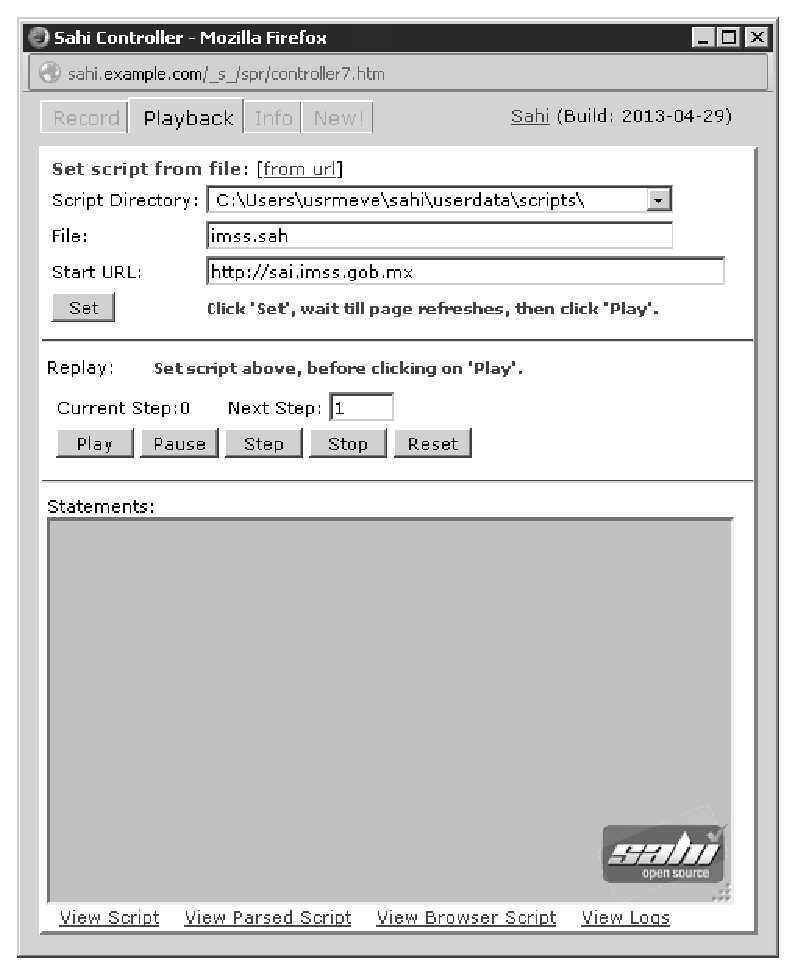
\includegraphics[scale=0.6]{ss-sahi-controller}
	\caption{Controlador de Sahi.}
	\label{fig:ss-sahi-controller}
	\end{figure}
\end{itemize}


\subsection{Lógica de automatización}
El componente de lógica de automatización provee de la información necesaria a las rutinas automatizadas, la información puede proceder de fuentes diferentes y cada una se accede de forma diferente:
\begin{enumerate}
 	\item Un archivo en el sistema de archivos del sistema operativo, se obtiene información utilizando el componente \textbf{Sistema de Archivos}.
 	\item Información almacenada en la base de datos, se tiene acceso miente el componente \textbf{Persistencia}.
 	\item Cálculos que corresponde a la lógica de negocio, estos datos se obtienen mediante la aplicación de reglas implementadas dentro del componente \textbf{Lógica de automatización}.
\end{enumerate}
La implementación de este componente ha sido escrita en el lenguaje de programación Java (ver sección \ref{sec-java}).\\
%Dado que la implementación a los datos en el sistema de archivos del sistema operativo y los almacenados en la base de datos son adquiridos mediante otros componentes, únicamente haré mención de la implementación de los datos que se obtienen por medio de reglas de negocio.
A continuación se muestran los puntos relevantes de la implementación de las interfaces mencionadas en la sección \ref{sec-logica-auto}:
\paragraph{\indent Interfaz Respuesta}
\begin{enumerate}
	\item guardar-orden-nueva: la implementación de esta operación (ver código \ref{lst:la-save-new}) muestra como se delega la aplicación del almacenamiento de una nueva orden de reposición al componente \textbf{Persistencia}\footnote{Para evitar redundancia en la explicación de la implementación del sistema AutoSA, en adelante no se mostrará más código que únicamente delegue la operación a otros componentes.}.
	\begin{lstlisting}[language=Java, caption={Delegación del almacenamiento de una nueva orden de reposición.}, label={lst:la-save-new}]
OrdenImss orden = new Orden();
orden.setContrato(contrato);
orden.setSolicitud(Long.parseLong(solicitud));
orden.setOrden(ordenLong);
orden.setFechaExpedicion(fechaExpedicion);
orden.setAlmacenDestino(Long.parseLong(almacenDestino));
orden.setUrlCon(urlCon);
orden.setUrlEnv(urlEnv);
orden.setEstatus(1);
orden.setIdSesionInsersion(idSesion);
orden.setIdSesionEstatus(idSesion);

ordenesDAO.insertOrden(orden);
	\end{lstlisting}

	\item obtener-datos-respuesta: la implementación del cálculo de fechas de fabricación y de caducidad descrita en el caso de uso \textbf{CU-RESPONDER-ORDEN} (ver sección \ref{cu-responder-orden}), código \ref{lst:la-dates} muestra el método en lenguaje Java:
	\begin{enumerate}
		\item En las líneas 2 a 7 se calcula el año para las fechas de fabricación y de caducidad.
		\item En las líneas 8 a 10 se construyen las fechas de fabricación y de caducidad.
	\end{enumerate}
	\begin{lstlisting}[language=Java, caption={Método para calcular las fechas de fabricación y caducidad.}, label={lst:la-dates}]
public String[] getFechasFab(){
	Calendar today = GregorianCalendar.getInstance();
	int anho;
	if(Calendar.DECEMBER == today.get(Calendar.MONTH)){
		anho = today.get(Calendar.YEAR) + 1;
	}else{
		anho = today.get(Calendar.YEAR);
	}
	String[] fechas = new String[2];
	fechas[0] = "01/01/" + anho;
	fechas[1] = "31/12/" + anho;
	
	return fechas;
}
	\end{lstlisting}

	\item obtener-acuse-envio: esta operación principalmente obtiene las rutas en el sistema de archivos para la generación del acuse de envío, posteriormente delega la generación del acuse al componente \textbf{Generación de reportes}. En el código \ref{lst:la-acuse} se muestra el código de Java que realiza los pasos anteriores.
	\begin{enumerate}
		\item La línea 1 estable el nombre del archivo como el número de la orden de reposición.
		\item La línea 2 obtiene la plantilla del acuse de envío para el Instituto de Salud.
		\item La línea 3 obtiene la ruta donde se depositan los archivos auxiliares en la generación del acuse de envío.
		\item Las líneas 4 a 7 construyen la ruta de directorios donde se depositará el acuse de envío.
		\item La línea 8 utiliza el componente \textbf{Generador de Reportes} para la creación del acuse de envío.
	\end{enumerate}
	\begin{lstlisting}[language=Java, caption={Generación del acuse de envío.}, label={lst:la-acuse}]
String filename = params.get("numorden");
String template = properties.getProperty("is.template.html");
File outhtmldir = new File(properties.getProperty("imss.output.dir"), filename + ".html");
SimpleDateFormat sdf = new SimpleDateFormat("yyyy MMMM dd", new Locale("es", "MX"));
String[] date = sdf.format(new Date()).split(" ");
File outputdir = new File(properties.getProperty("is.output.pdf"), String.format(REPORT_DIR_TMPL, date[0], date[1], date[2]));
outputdir.mkdirs();
snapShotService.takeSnapShot(params, filename, template, outhtmldir, outputdir);
	\end{lstlisting}

\end{enumerate}
\paragraph{\indent Interfaz Verificación}
\begin{enumerate}
	\item obtener-rango-fechas-verificar: el código \ref{lst:la-date-search} muestra el cálculo de las fechas necesarias para el formulario de búsqueda de órdenes de reposición.
	\begin{enumerate}
		\item La línea 5 muestra la obtención de la fecha mayor (día actual).
		\item La líneas 6 y 7 muestran la obtención de la fecha menor (60 días antes de la fecha actual).
	\end{enumerate}
	\begin{lstlisting}[language=Java, caption={Cálculo del rango de fechas para buscar órdenes de reposición canceladas.}, label={lst:la-date-search}]
DateFormat dateFormat = new SimpleDateFormat(format);
Calendar cal = GregorianCalendar.getInstance();
String[] dates = new String[2];
dates[1] = dateFormat.format(cal.getTime());
cal.add(Calendar.DAY_OF_YEAR, -60);
dates[0] = dateFormat.format(cal.getTime());
	\end{lstlisting}

	\item actualizar-estado-sa: Esta operación realiza la actualización de las órdenes de reposición canceladas, en el código \ref{lst:la-validate} muestra el código Java.
	\begin{enumerate}
		\item La línea 1 obtiene las órdenes de reposición canceladas del listado de órdenes de reposición encontradas.
		\item La línea 2 actualiza el estado de las órdenes de reposición.
	\end{enumerate}
	\begin{lstlisting}[language=Java, caption={Actualización de órdenes de reposición canceladas.}, label={lst:la-validate}]
	List<Orden> ordenes = xmlReader.getCancelled(htmlTable);
	persistence.updateSaiStatus(ordenes, status);
	\end{lstlisting}
\end{enumerate}


\subsection{Persistencia}
\subsubsection{Tecnologías utilizadas}
\textcolor{blue}{
\begin{enumerate}
	\item JDBC 			(Patrón factory)
	\item JPA			(Patrón proxy)
	\item SpringData	(Patrón proxy)
\end{enumerate}
}


\subsection{Sistema de archivos}
	\paragraph{Configuración\\}
		\textbf{obtener-propiedad}
	\paragraph{Almacenamiento\\}
		\textbf{guardar-archivo}


\subsection{Generador de reportes}

\textcolor{blue}{En el diseño debe agregarse un diagrama del funcionamiento de reportes: seleccionar templates... agregar patrones de diseño}\\
\subsection{Motor de plantillas}
\textcolor{blue}{aquí platico de volicity y como funciona el motor}\\
\textcolor{blue}{aquí va la configuración}\\
\textcolor{blue}{tipos de reporte}

	\paragraph{Acuse\\}
		\textbf{generar-acuse-envio}
	\paragraph{Generación\\}
 		\textbf{generar-reporte-ordenes}


\subsection{Portal Web}
\textcolor{blue}{Las secciones de esta parte serán presentadas por capas desde datos hasta la vista}\\
\textcolor{blue}{Presentar el patron MVC}\\
\subsection{Acceso}
\textcolor{blue}{Spring security}\\
\textcolor{blue}{Cifrado de contraseña}\\
\subsection{Generación de reportes}
\subsection{Búsqueda}

\subsection{Administración de catálogos}

\subsection{Visualización de órden de reposición}

\subsection{Edición de órden de reposición}









%\section{Implmenetación de genración de reportes}

%\section{Implementación de automatización para SA}
%\subsection{Bibliotecas para las rutinas de automatización}
%\subsection{Rutinas de automatización}






\renewcommand{\appendixname}{Apéndice}
\renewcommand{\appendixtocname}{Apéndices}
\renewcommand{\appendixpagename}{Apéndices}
\begin{appendices}
%\chapter{Diccionario de Datos}


\section{Tablas}

\paragraph*{sesion} Define una sesión bajo la cual se ejecuta un script de automatización, la sesión puede definir implísitamente un usuario y un rol.
\begin{longtable}{p{4cm}|l|p{8.5cm}}
	\textbf{Columna} &	\textbf{Tipo} &	\textbf{Descripción} \\
	\hline\hline
	{\fontfamily{pcr}\selectfont id}& number & Número identificador \\
	\hline
	{\fontfamily{pcr}\selectfont id{\textunderscore}usuario} & number & Identificador de usuario que creó la sesión \\
	\hline
	{\fontfamily{pcr}\selectfont fecha{\textunderscore}creacion} & datetime & Hora y fecha en que se registró la sesión. Default: CURRENT{\textunderscore}TIMESTAMP \\ 
	\hline
	{\fontfamily{pcr}\selectfont id{\textunderscore}usuario{\textunderscore}fin} & number & Identificador de usuario que finalizó la sesión \\
	\hline
	{\fontfamily{pcr}\selectfont fecha{\textunderscore}fin} & datetime & Hora y fecha en que se finalizó la sesión\\
	\hline
	{\fontfamily{pcr}\selectfont activa} & number & Indicador de actividad en la sesión. Default: 1\\
	\hline
	{\fontfamily{pcr}\selectfont rol} & number & Rol para el cuál fue creada la sesión.\\
	\caption{Tabla sesion.}\label{tab:tab-sesion}
\end{longtable}

\paragraph*{bitacora} Lleva el registro de eventos ocurridos durante la ejecución del script de automatización, el evento puede estar ligado a una sesión.
\begin{longtable}{p{4cm}|l|p{8.5cm}}
	\textbf{Columna} &	\textbf{Tipo} &	\textbf{Descripción} \\
	\hline\hline
	{\fontfamily{pcr}\selectfont id} & number & Número identificador\\
	\hline
	{\fontfamily{pcr}\selectfont id{\textunderscore}sesion} & number & Identificador de sesión desde la cual se hizo el registro.\\
	\hline
	{\fontfamily{pcr}\selectfont fecha} & datetime & Hora y fecha en la que se realizó el registro Default: CURRENT{\textunderscore}TIMESTAMP\\
	\hline
	{\fontfamily{pcr}\selectfont descripcion} & text & Descripción del evento.\\
\caption{Tabla bitacora.}\label{tab:tab-bitacora}
\end{longtable}

\paragraph*{ordenes{\textunderscore}imss} Contiene el registro de las órdenes de reposición del portal SAI que han sido procesadas por el script de automatización.
%\begin{landscape}
\begin{longtable}{p{4cm}|l|p{8.5cm}}
	\textbf{Columna} &	\textbf{Tipo} &	\textbf{Descripción} \\
	\hline\hline
	{\fontfamily{pcr}\selectfont id} & number & Número identificador\\
	\hline
	{\fontfamily{pcr}\selectfont contrato} & text & Cadena alfanumérica con el identificador de contrato\\
	\hline
	{\fontfamily{pcr}\selectfont solicitud} & number & Número de solicitud\\
	\hline
	{\fontfamily{pcr}\selectfont orden} & number & Número de orden de reposición\\
	\hline
	{\fontfamily{pcr}\selectfont fecha{\textunderscore}expedicion} & text & Fecha de expedición\\
	\hline
	{\fontfamily{pcr}\selectfont almacen{\textunderscore}destino} & number & Número identificador del almacén destino\\
	\hline
	{\fontfamily{pcr}\selectfont estatus} & number & Estatus en el proceso de atención Default: 1\\
	\hline
	{\fontfamily{pcr}\selectfont cbb} & number & Clave de Cuadro Básico\\
	\hline
	{\fontfamily{pcr}\selectfont fecha{\textunderscore}vencimiento} & text & Fecha de vencimiento\\
	\hline
	{\fontfamily{pcr}\selectfont cantidad} & number & Cantidad solicitada\\
	\hline
	{\fontfamily{pcr}\selectfont fecha{\textunderscore}insersion} & datetime & Fecha en la que fue registrada la orden en la base de datos. Default: CURRENT{\textunderscore}TIMESTAMP\\
	\hline
	{\fontfamily{pcr}\selectfont fecha{\textunderscore}estatus} & datetime & Fecha en la que se registró el último cambio de estatus Default: CURRENT{\textunderscore}TIMESTAMP\\
	\hline
	{\fontfamily{pcr}\selectfont id{\textunderscore}sesion{\textunderscore} insersion} & number & Identificador de la sesión que realizó el registro en la base de datos\\
	\hline
	{\fontfamily{pcr}\selectfont id{\textunderscore}sesion{\textunderscore}estatus} & number & Identificador de la sesión que realizó el último cambio de estatus\\
	\hline
	{\fontfamily{pcr}\selectfont url{\textunderscore}con} & text & URL de SAI para realizar la contestación\\
	\hline
	{\fontfamily{pcr}\selectfont url{\textunderscore}env} & text & URL de SAI para realizar el envío\\
	\hline
	{\fontfamily{pcr}\selectfont confirmacion} & number & Número de confirmación de envío\\
	\hline
	{\fontfamily{pcr}\selectfont articulo} & text & Artículo según la descripción del campo en la pantalla de finalización de SAI\\
	\hline
	{\fontfamily{pcr}\selectfont unidad} & text & Unidad a la que se refiere la cantidad solicitada según la pantalla de finalización de SAI\\
	\hline
	{\fontfamily{pcr}\selectfont precio} & number & Precio por unidad\\
	\hline
	{\fontfamily{pcr}\selectfont lugar{\textunderscore}entrega} & text & Lugar de entrega\\
	\hline
	{\fontfamily{pcr}\selectfont lote} & text & Identificador del lote\\
	\hline
	{\fontfamily{pcr}\selectfont fecha{\textunderscore}fabricacion} & text & Fecha de fabricación\\
	\hline
	{\fontfamily{pcr}\selectfont fecha{\textunderscore}caducidad} & text & Fecha de caducidad\\
	\hline
	{\fontfamily{pcr}\selectfont marca} & text & La marca del medicamento como se describe en la pantalla de contestación\\
	\hline
	{\fontfamily{pcr}\selectfont procedencia} & text & La procedencia del medicamento como se describe en la pantalla de contestación\\
	\hline
	{\fontfamily{pcr}\selectfont estatus{\textunderscore}sai} & number & Estatus de la orden de reposición en el portal SAI\\
	\hline
	{\fontfamily{pcr}\selectfont estatus{\textunderscore}sap} & number & Estatus de la orden de reposición en el sistema interno de MAYPO\\

	\caption{Tabla ordenes{\textunderscore}imss.}\label{tab:tab-ordenes-imss}
\end{longtable}
%\end{landscape}

\paragraph*{cat{\textunderscore}estatus{\textunderscore}orden} Este catálogo no debe ser alterado, contiene los posibles estatus que pude tomar una orden durante el ciclo de vida de la aplicación.
\begin{longtable}{p{4cm}|l|p{8.5cm}}
	\textbf{Columna} &	\textbf{Tipo} &	\textbf{Descripción} \\
	\hline\hline
	{\fontfamily{pcr}\selectfont id} & number & Número identificador \\
	\hline
	{\fontfamily{pcr}\selectfont nombre} & text & Nombre corto del estatus\\
	\caption{Tabla cat{\textunderscore}estatus{\textunderscore}orden.}\label{tab:tab-cat-estatus-orden}
\end{longtable}

\paragraph*{cat{\textunderscore}estatus{\textunderscore}sai} Este catálogo contiene los estados definidos por el portal SAI para una orden de reposición.
\begin{longtable}{p{4cm}|l|p{8.5cm}}
	\textbf{Columna} &	\textbf{Tipo} &	\textbf{Descripción} \\
	\hline\hline	
	{\fontfamily{pcr}\selectfont id} & number & Número identificador \\
	\hline
	{\fontfamily{pcr}\selectfont nombre} & text & Nombre corto del estatus\\
	\caption{Tabla cat{\textunderscore}estatus{\textunderscore}sai.}\label{tab:tab-cat-estatus-sai}
\end{longtable}

\paragraph*{cat{\textunderscore}clientes} Este catálogo refleja el contenido necesario para la generación del layout de SAP ubicado en la hoja CLIENTES del archivo LICITACION  CARGA IMSS 2014.xlsx.
\begin{longtable}{p{4cm}|l|p{8.5cm}}
	\textbf{Columna} &	\textbf{Tipo} &	\textbf{Descripción} \\
	\hline\hline	
	{\fontfamily{pcr}\selectfont lugar{\textunderscore}entrega} & number & Columna A, LUGAR DE ENTREGA\\
	\hline
	{\fontfamily{pcr}\selectfont factura} & number & Columna B, FACTURA\\
	\hline
	{\fontfamily{pcr}\selectfont destino}  & number & Columna C, DESTINO\\
	\hline
	{\fontfamily{pcr}\selectfont consignado{\textunderscore} controlado}  & number & Columna D, CONSIGNADO CONTROLADO\\
	\hline
	{\fontfamily{pcr}\selectfont almacen} & text & Columna E, ALMACEN \\
	\hline
	{\fontfamily{pcr}\selectfont entrega} & text & Columna F, ENTREGA\\
	\caption{Tabla cat{\textunderscore}clientes.}\label{tab:tab-cat-clientes}
\end{longtable}

\paragraph*{cat{\textunderscore}contratos} Este catálogo refleja el contenido necesario para la generación del layout de SAP ubicado en la hoja CONTRATOS del archivo LICITACION  CARGA IMSS 2014.xlsx.
\begin{longtable}{p{4cm}|l|p{8.5cm}}
	\textbf{Columna} &	\textbf{Tipo} &	\textbf{Descripción} \\
	\hline\hline	
	{\fontfamily{pcr}\selectfont pedido} & text & Columna B, No PEDIDO\\
	\hline
	{\fontfamily{pcr}\selectfont documento{\textunderscore} comercial} & number & Columna C, DOCUMENTO  COMERCIAL\\
	\hline
	{\fontfamily{pcr}\selectfont cbb} & number & Columna F, CCB\\
	\hline
	{\fontfamily{pcr}\selectfont material} & number & Columna G, MATERIAL\\
	\hline
	{\fontfamily{pcr}\selectfont tipo} & text & Columna I, TIPO\\
	\hline
	{\fontfamily{pcr}\selectfont etiqueta} & text & Columna Q, ETIQUETA\\
	\hline
	{\fontfamily{pcr}\selectfont fianza} & number & Columna U, FIANZA\\
	\caption{Tabla cat{\textunderscore}contratos.}\label{tab:tab-cat-contratos}
\end{longtable}


\section{Vistas}
\paragraph*{matriz{\textunderscore}imss} Esta vista refleja el contenido necesario para la generación del layout de SAP ubicado en la hoja MATRIZ del archivo LICITACION  CARGA IMSS 2014.xlsx.
\begin{longtable}{p{4cm}|l|p{8.5cm}}
	\textbf{Columna} &	\textbf{Tipo} &	\textbf{Descripción} \\
	\hline\hline
	{\fontfamily{pcr}\selectfont documento{\textunderscore} comercial} & number & El máximo de la columna documento{\textunderscore}comercial de los renglones del catálogo de contratos cuyos contrato y CCB sean iguales sean iguales a los de la orden de reposición.\\
	\hline
	{\fontfamily{pcr}\selectfont fianza} & number & El máximo de la columna fianza de los renglones del catálogo de contratos cuyos contrato y CCB sean iguales sean iguales a los de la orden de reposición.\\
	\hline
	{\fontfamily{pcr}\selectfont solicitud} & number & Columna solicitud de la orden.\\
	\hline
	{\fontfamily{pcr}\selectfont fecha{\textunderscore}expedicion} & text & Columna fecha{\textunderscore}expedicion de la orden.\\
	\hline
	{\fontfamily{pcr}\selectfont orden} & number & Columna orden de la orden de reposición.\\
	\hline
	{\fontfamily{pcr}\selectfont factura} & number & El máximo de la columna factura de los renglones del catálogo de clientes cuyo almacén destino de la orden de reposición sea igual al lugar de entrega del catálogo.\\
	\hline
	{\fontfamily{pcr}\selectfont cte{\textunderscore}destino} & number & Sí el tipo del contrato de la orden de reposición es CONTROLADO, entonces se debe tomar el máximo valor de la columna consigando{\textunderscore}controlado del catálogo de clientes cuyo almacén destino de la orden de reposición sea igual al lugar de entrega del catálogo. En caso contrario se debe tomar el máximo de la columna destino con los mismos criterios del caso anterior.\\
	\hline
	{\fontfamily{pcr}\selectfont entrega} & text & El máximo de la columna entrega de los renglones del catálogo de clientes cuyo almacén destino de la orden de reposición sea igual al lugar de entrega del catálogo.\\
	\hline
	{\fontfamily{pcr}\selectfont material} & number & El máximo de la columna material de los renglones del catálogo de contratos cuyos contrato y CCB sean iguales sean iguales a los de la orden de reposición.\\
	\hline
	{\fontfamily{pcr}\selectfont instrucciones{\textunderscore} etiquetado} & text & Columna U, INSTRUCCIONES DE ETIQUETADO  (archivo Excel)
El máximo de la concatenación de las columnas etiqueta y cbb (separadas por un espacio) de los renglones del catálogo de contratos cuyos contrato y CCB sean iguales a los de la orden de reposición.\\
	\hline
	{\fontfamily{pcr}\selectfont cantidad} & number & Cantidad solicitada de la orden de reposición\\
	\hline
	{\fontfamily{pcr}\selectfont fecha{\textunderscore}vencimiento} & text & Fecha de vencimiento de la orden de reposición\\
	\hline
	{\fontfamily{pcr}\selectfont sesion} & number & Sesión con la cual fue finalizada la orden de reposición, esta columna no está contenida en el archivo de Excel. Identificador de la sesión que realizó el último cambio de estatus.\\
	\caption{Tabla matriz{\textunderscore}imss.}\label{tab:tab-matriz-imss}
\end{longtable}

\paragraph*{layout{\textunderscore}imss{\textunderscore}sap} Esta vista refleja el contenido de la hoja Formato de carga SAP del archivo CARGA MASIVA IMSS HECTOR.xlsm después de haber aplicado la macro que contiene sobre el archivo LICITACION  CARGA IMSS 2014.xlsx.
\begin{longtable}{p{4cm}|l|p{8.5cm}}
	\textbf{Columna} &	\textbf{Tipo} &	\textbf{Descripción} \\
	\hline\hline
	{\fontfamily{pcr}\selectfont documento{\textunderscore} comercial} & number & Columna A, DSADAS Columna documento{\textunderscore}comercial de vista matriz{\textunderscore}imss\\
	\hline
	{\fontfamily{pcr}\selectfont solicitante} & number & Columna B, Solicitante Valor constante 100002\\
	\hline
	{\fontfamily{pcr}\selectfont solicitud} & number & Columna C, SOLICITUD Columna solicitud de vista matriz{\textunderscore}imss\\
	\hline
	{\fontfamily{pcr}\selectfont fecha{\textunderscore}expedicion} & text & Columna D, FECHA DE EXPEDICIÓN Columna fecha{\textunderscore}expedicion de vista matriz{\textunderscore}imss\\
	\hline
	{\fontfamily{pcr}\selectfont orden} & number & Columna E, ORDEN REPOSICIÓN Columna orden de vista matriz{\textunderscore}imss\\
	\hline
	{\fontfamily{pcr}\selectfont factura} & number & Columna F, CTE FACTURA Columna factura de vista matriz{\textunderscore}imss\\
	\hline
	{\fontfamily{pcr}\selectfont cte{\textunderscore}destino} & number & Columna G, CTE DESTINO Columna cte{\textunderscore}destino de vista matriz{\textunderscore}imss\\
	\hline
	{\fontfamily{pcr}\selectfont material} & number & Columna H, MATERIAL SAP Columna material de vista matriz{\textunderscore}imss\\
	\hline
	{\fontfamily{pcr}\selectfont instrucciones{\textunderscore} etiquetado} & number & Columna I, INTRUCCIONES DE ETIQUETADO Columna instrucciones{\textunderscore}etiquetado de vista matriz{\textunderscore}imss\\
	\hline
	{\fontfamily{pcr}\selectfont cantidad} & number & Columna J, CANTIDAD SOLICITADA Columna cantidad de vista matriz{\textunderscore}imss\\
	\hline
	{\fontfamily{pcr}\selectfont fecha{\textunderscore}limite} & text & Columna K, FECHA LÍMITE Columna fecha{\textunderscore}vencimiento de vista matriz{\textunderscore}imss\\
	\hline
	{\fontfamily{pcr}\selectfont fianza} & number & Columna L, Número de fianza Columna fianza de vista matriz{\textunderscore}imss\\
	\hline
	{\fontfamily{pcr}\selectfont fecha{\textunderscore}preferente} & text & Columna M, Fecha preferente de entrega Columna fecha{\textunderscore}vencimiento de vista matriz{\textunderscore}imss\\
	\hline
	{\fontfamily{pcr}\selectfont entrega} & text & Columna N, Instrucciones para distribución Columna entrega de vista matriz{\textunderscore}imss\\
	\hline
	{\fontfamily{pcr}\selectfont sesion} & number & Sesión con la cual fue finalizada la orden de reposición, esta columna no está contenida en el archivo de Excel.\\
	\caption{Tabla layout{\textunderscore}imss{\textunderscore}sap.}\label{tab:tab-layout-imss-sap}
\end{longtable}
\chapter{Unified Modeling Language}
\textcolor{blue}{Lenguaje de Modelado Unificado (UML por sus siglas en inglés).}
\textcolor{red}{Mejorar la definición porque está muy pitera.}
\textcolor{red}{No mentiré, toda esta sección será un homenaje a este libro \cite{SoftwareEngineeringUML}}
\section{Diagrama de casos de uso}\label{sec-uml-cu}
\textcolor{blue}{lalalalalala}
\section{Diagrama de actividad}\label{sec-uml-act}
\textcolor{blue}{lalalalalala}
\section{Diagrama de componentes}\label{sec-uml-comp}
\textcolor{blue}{lalalalalala}
\section{Diagrama de paquetes}\label{sec-uml-pack}
\textcolor{blue}{lalalalalala}
\section{Diagrama de secuencia}\label{sec-uml-seq}
\textcolor{blue}{lalalalalala}


\chapter{Técnicas de Diseño}\label{sec-patrones}

\section{Patrones de Diseño}
``Un patrón describe un problema recurrente sobre un ambiente, y entonces describe la técnica que soluciona el problema de forma tal que puede ser utilizado sobre cualquier instancia del problema''\cite{DesignPatterns}, es decir, que dados los requerimientos funcionales del sistema es posible analizar la comunicación entre sus distintas partes y de esta forma saber lo patrones que son útiles para dar solución. Los patrones son organizados en tres categorías\cite{DesignPatterns}:
\begin{itemize}
	\item \textbf{Creacionales}: describen la forma en que las entidades (objetos si se utiliza el paradigma orientado a objetos) del sistema son creadas.
	\item \textbf{Estructurales}: describen la organización entre las entidades del sistema.
	\item \textbf{Comportamiento}: describen la comunicación entre entidades del sistema
\end{itemize}

\section{Patrón Objeto de Acceso a Datos}\label{sec-dao}
El patrón Objeto de Acceso a Datos (DAO por sus siglas en inglés) encapsula y abstrae la conexión a una fuente de datos (archivos de texto plano, bases de datos relacionales, bases de datos no relacionales, etc.) y expone operaciones pertinentes al manejo de tales datos\cite{OCPJavaSE7,OCAPJavaSE7}:
\begin{enumerate}
	\item [] \textbf{buscar}: Realiza la búsqueda de un único elemento, en caso de no encontrarse tal elemento la respuesta es nula.
	\item [] \textbf{listar}: Extrae todos los elementos, el resultado puede utilizar estrategias de paginación.
	\item [] \textbf{insertar}: Guarda un nuevo elemento en la fuente de datos.
	\item [] \textbf{actualizar}: Actualiza la información de un elemento existente en la fuente de datos.
	\item [] \textbf{borrar}: Borra el registro de un elemento en la fuente de datos.
\end{enumerate}


\section{Patrón Modelo-Vista-Controlador}\label{sec-mvc}
Para Sarcar\cite{JavaDesignPatternsExamples} el patrón Modelo Vista Controlador (MVC) es un patrón de arquitectura que consiste de tres grandes componentes: Modelo, Vista y Controlador. El Controlador conduce la comunicación entre la Vista y el Modelo, en la Figura \ref{fig:dia-mvc-simple} se muestra el flujo de comunicación entre los componentes MVC.
\begin{enumerate}
	\item \textbf{Modelo}: tiene la responsabilidad de manejar el acceso a los datos persistentes y la lógica de negocio, usualmente se acompaña del patrón DAO\footnote{Ver sección \ref{sec-dao}} para el manejo de datos.
	\item \textbf{Vista}: es la capa de presentación, es responsable de mostrar los datos al actor\footnote{Puede ser una persona u otro sistema} que use el sistema.
	\item \textbf{Controlador}: es el intermediario entre la Vista y el Modelo: comunica las peticiones de la vista al modelo y los datos del modelo a la vista.
\end{enumerate}
\begin{figure}[h]
  \centering
  \includegraphics[scale=0.4]{dia-mvc-simple}
  \caption{Diagrama del patrón MVC\cite{JavaDesignPatternsExamples}.}
  \label{fig:dia-mvc-simple}
\end{figure}


\iffalse
\section{Arquitectura 4+1} Organiza cada decisión en el diseño del sistema en cuatro partes llamadas vistas (ver Figura \ref{fig:dia-arq-4-1}), cada vista se encarga de enfocarse en un aspecto del diseño, estas cuatro vistas son unificadas por una cuarta vista de escenarios o casos de uso\cite{ViewModel4plus1}:
\begin{itemize}
	\item \textbf{Vista Lógica}: son las reglas del negocio por las que se rige la operación del usuario final.
	\item \textbf{Vista de Proceso}: refleja concurrencia y sincronización.
	\item \textbf{Vista de Física}: describe las relaciones del software con el hardware.
	\item \textbf{Vista de Desarrollo}: describe la organización estática del software en su ambiente de desarrollo.
\end{itemize}

\begin{figure}[h]
\centering
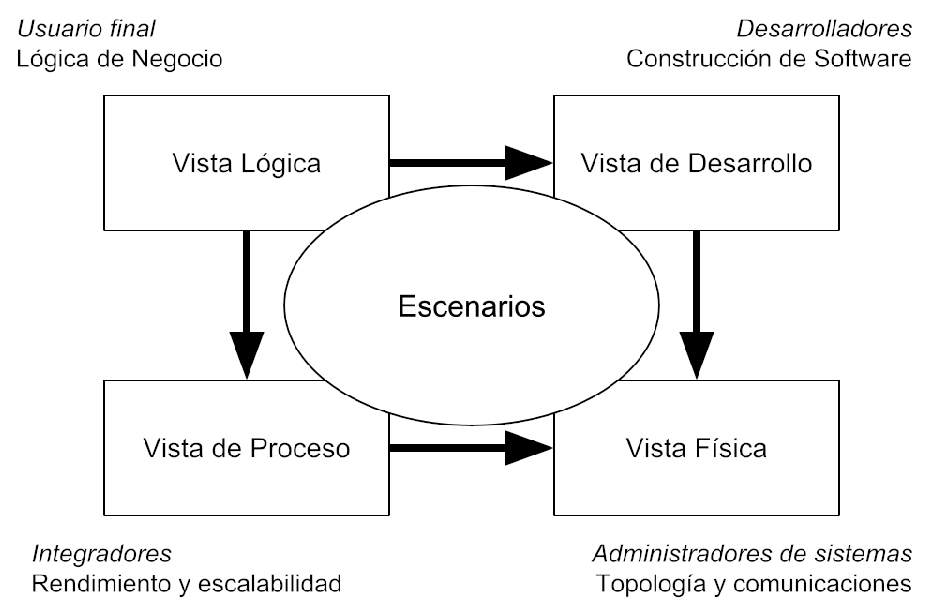
\includegraphics[scale=0.5]{dia-arq-4-1} 
\caption{Diagrama de arquitectura 4+1.\cite{ViewModel4plus1}}
\label{fig:dia-arq-4-1}
\end{figure}


\section{Arquitectura Orientada a Servicios}
Thomas Erl describe la Arquitectura Orientada a Servicios (\textbf{SOA} por sus siglas en inglés) como el modelo arquitectónico del cómputo orientado a servicios\cite{SOAWithRest}, a continuación se muestran las definiciones de Erl sobre los conceptos de Orientación a Servicios:
\begin{quote}
La \textbf{Orientación a Servicios} es el paradigma de diseño dedicado para la creación de unidades lógicas de solución que son moldeados individualmente para que puedan ser utilizados colectiva y repetidamente para la realización de objetivos estratégicos y beneficios asociados con el cómputo orientado a servicios.\\
El \textbf{Cómputo Orientado a Servicios} es engloba distintas plataformas de cómputo distribuido. En sí envuelve su propio paradigma y principios de diseño, catálogos de diseño de patrones, lenguajes, modelo arquitectónico junto con sus conceptos relacionados, tecnologías y marcos de trabajo.\\
La \textbf{Arquitectura Orientada a Servicios} es un modelo de tecnología arquitectónica para soluciones orientadas a servicios con distintas características en apoyo de realizar orientación a servicios y los objetivos estratégicos asociados con el cómputo orientado a servicios.\cite{SOAWithRest}
\end{quote}
\fi

\end{appendices}

%Bibliografia
\renewcommand{\bibname}{Bibliografía}
%\nocite{*} 
%\bibliographystyle{apacite}
\bibliographystyle{acm}
\bibliography{Bibliografia}
\end{document}